%!TEX root = CAN.tex
\section{Timing Calibration}

To perform the timing calibration of the AHCAL, the complete muon dataset is used. The electron dataset is used in a next step to validate the calibration procedure as described in subsection \ref{subsec:validation}. Table \ref{table:mu_elec_runs} summarises the runs and datasets used. Raw events are considered if the reference signals T$_{12}$,  T$_{13}$ and T$_{14}$ are present in the event. Selected events are counted after the selection on the error of the time reference as explained in \ref{subsection:time_ref}.
\begin{table}[htbp]
\centering
\resizebox{0.9\textwidth}{!}{%
  \begin{tabular}{@{} llllll @{}}
    \hline
    Runs & Energy & Particle Type & Events (Raw) & Events (sel.) & $\frac{\text{N$_{sel.}$}}{\text{N$_{raw}$}}$ \\
    \hline
     24016-24663 & 50-150 GeV & $\mu^-$ & 1851536 & 836796 & 45.2\% \\
     24528-24577 & 10 GeV & $e^-$ & 268275 & 216656 & 80.8\% \\
     24510-24520 & 15 GeV & $e^-$ & 108092 & 90395 & 83.6\% \\
     24486-24504 & 20 GeV & $e^-$ & 130232 & 110161 & 84.6\% \\
     24460-24470 & 30 GeV & $e^-$ & 82202 & 69692 & 84.8\% \\
     24427-24435 & 40 GeV & $e^-$ & 65901 & 55660 & 84.5\% \\
     24405-24419 & 50 GeV & $e^-$ & 123422 & 104030 & 84.3\% \\
    \hline
  \end{tabular}
  }
  \caption{Table with the statistic before and after selection used for timing calibration.}
  \label{table:mu_elec_runs}
\end{table}

\subsection{Slope calibration}
\label{subsec:slope_calib}

The data analysis is performed in several steps. The first step is the calibration of the time provided by the SPIROC2B chip. To reconstruct the time of the first hit (only a single hit per channel is registered during a bunch-crossing) in a channel, the TDC value measured needs to be converted into nanoseconds. The value is converted using the following equations:
\begin{equation} \label{eq:slope}
\text{slope}_{chip, BXID} \: \text{[ns/TDC]} = \frac{3920 \: \text{ns}}{\text{Max}_{chip, BXID} - \text{Pedestal}_{chip, BXID}}
\end{equation}
\begin{equation} \label{eq:time_chn}
\text{T}_{chn} \: \text{[ns]} = \text{slope}_{chip, BXID} \times (\text{TDC} - \text{Pedestal}_{mem=1} )
\end{equation}

The determination of the parameter $\text{slope}_{chip, BXID}$ is assuming that the TDC ramp is linear. The parameters Max$_{chip, BXID}$ and Pedestal$_{chip, BXID}$ in eq.\ref{eq:slope} are extracted from the TDC spectrum from a specific chip and BXID using only the first memory cell as illustrated in figure \ref{fig:TDC_Spectrum}. At the same time, the parameter Pedestal$_{mem=1}$ in eq.\ref{eq:time_chn} is extracted from the spectrum for each channel and the first memory cell of a chip without taking into account the BXID of the ramp as the difference between both pedestal can be corrected for at a later stage. This is accounting for a total of 208 slopes and 3744 pedestals to be extracted for the testbeam setup.
\begin{figure}[!htbp]
	\subfigure[TDC Spectrum of a typical chip.\label{fig:TDC_Spectrum}] {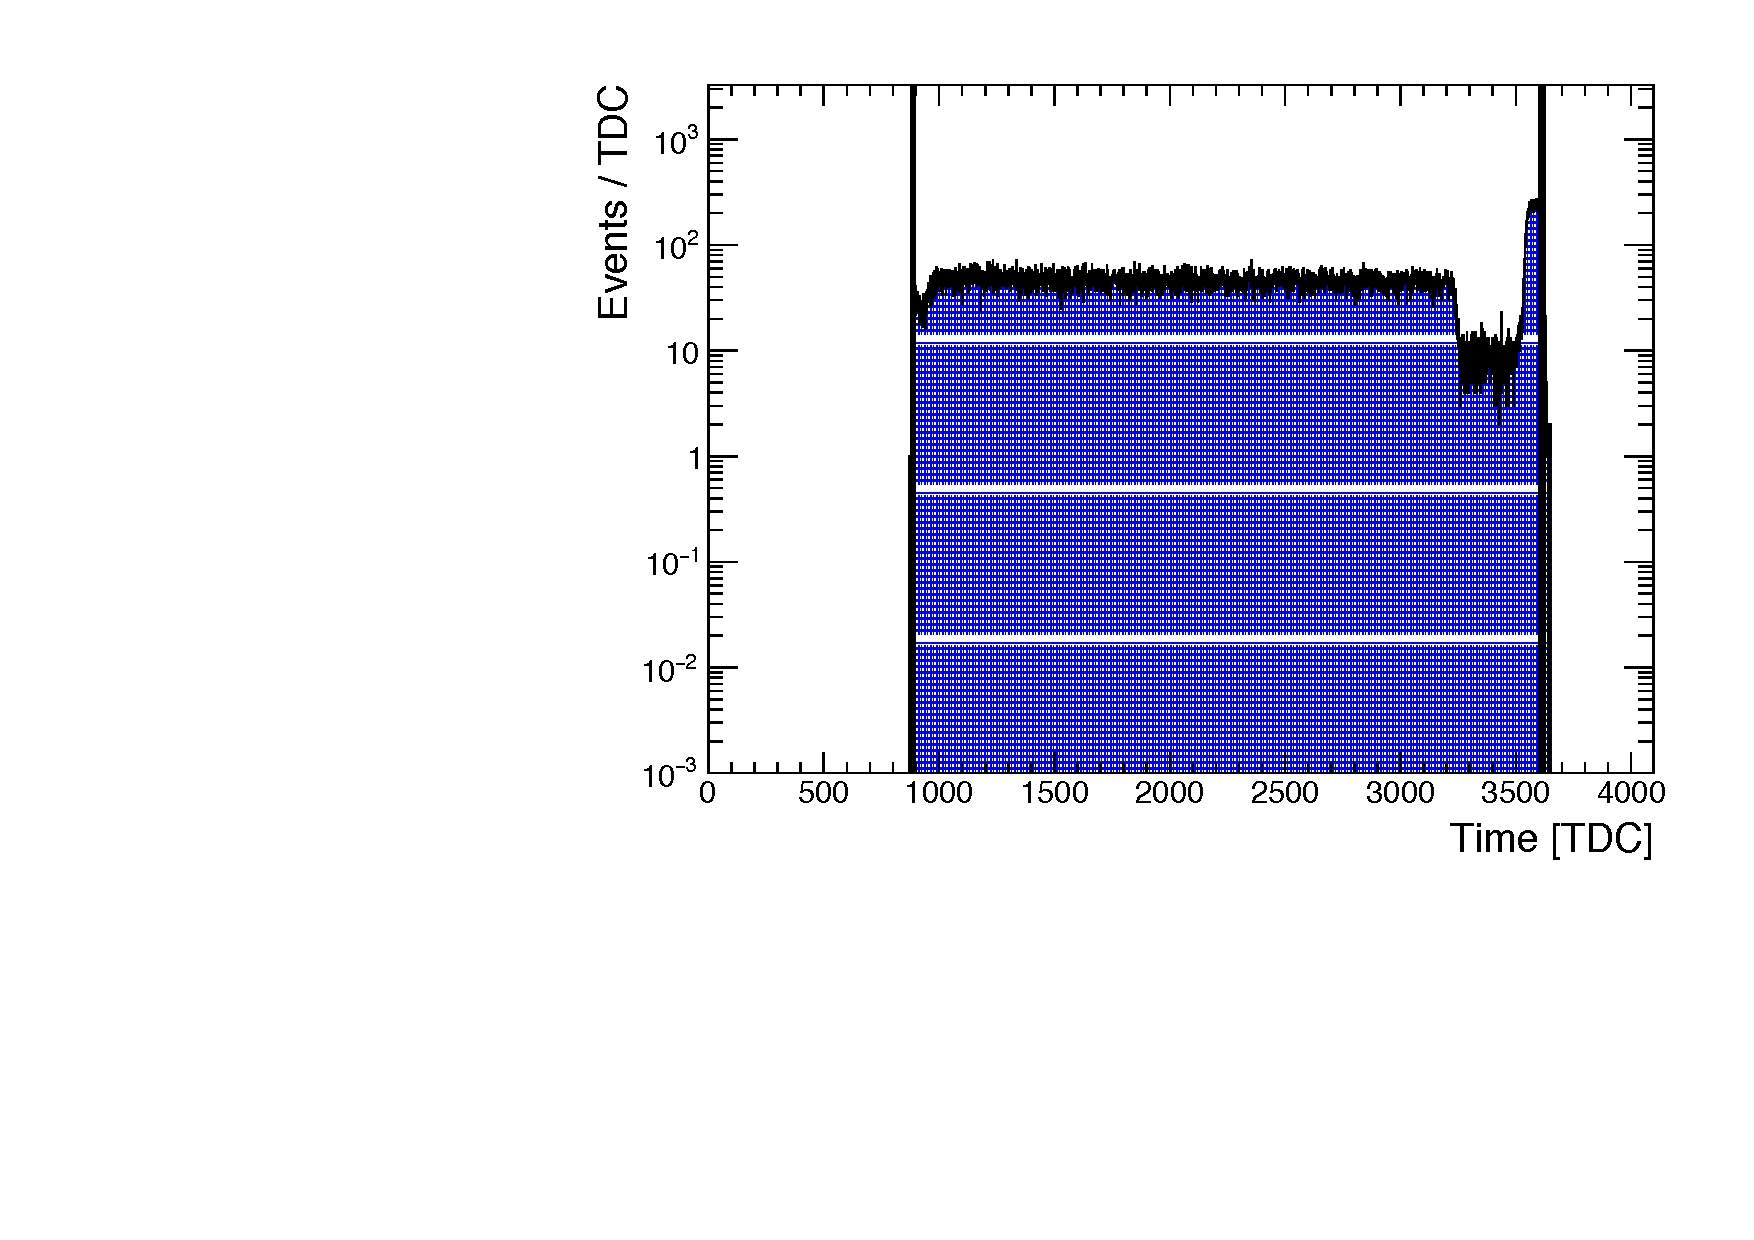
\includegraphics[width=0.5\textwidth]{fig/Muons/ExampleTDCSpectra.pdf}}\hfill
	\subfigure[Distribution of the fitted slopes for even and odd bunch-crossing IDs.\label{fig:slope_time}] {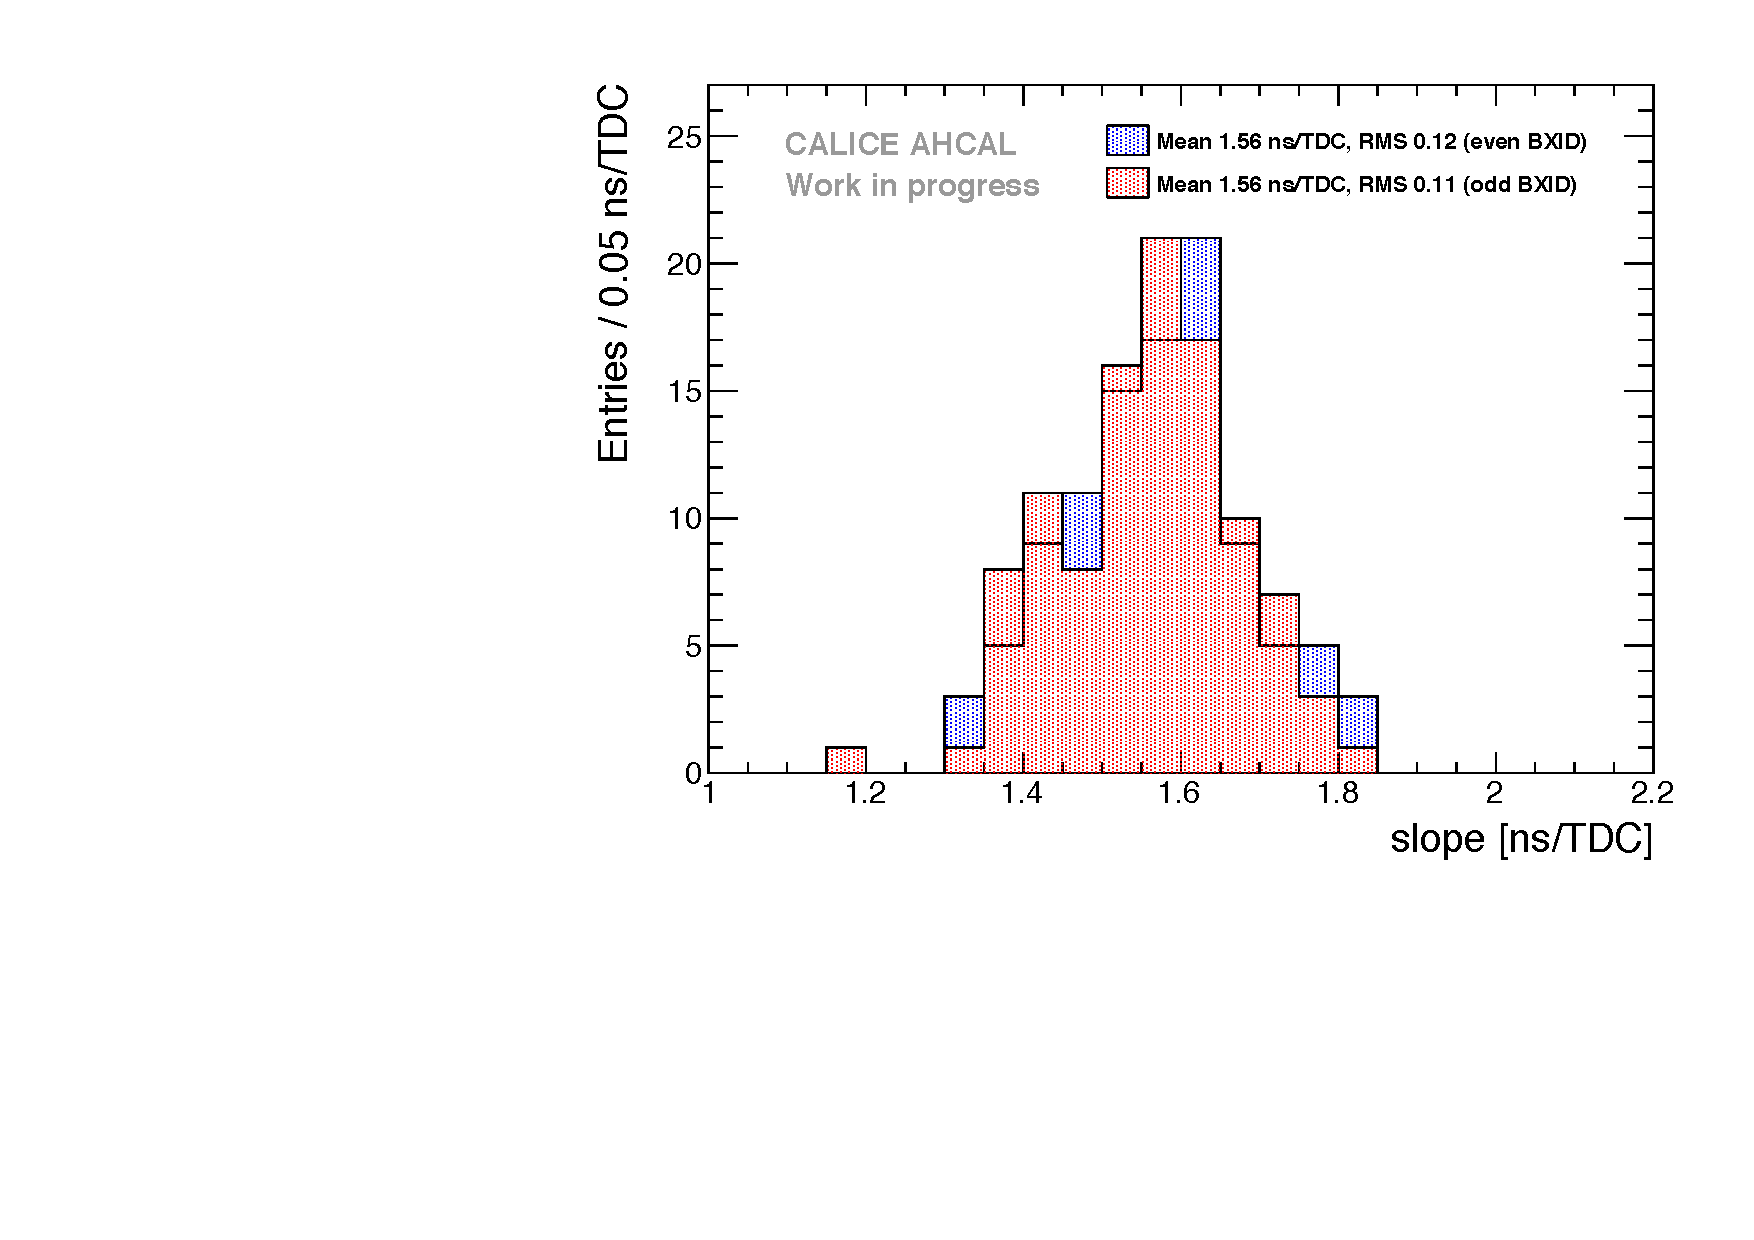
\includegraphics[width=0.5\textwidth]{fig/Muons/SlopesTDC.pdf}}
	\caption[]{\textbf{a}: The red rectangle are the fitted Max and Pedestal parameters for this chip. The yellow bands represents estimation of the error made on the extraction of the parameters by a variation of 1 RMS of the threshold $\mu$. The parameters extracted are slope = 1.56 $\pm$ 0.01, Pedestal = 816 $\pm$ 9 and Maximum = 3336 $\pm$ 8. \textbf{b}: $\mu_{odd}$ = 1.564 ns/TDC, RMS$_{odd}$ = 0.121, $\mu_{even}$ = 1.556 ns/TDC, RMS$_{even}$ = 0.113.}
\end{figure}

The technique of extraction is based on an edge detection method. For each chip and BXID, an histogram is filled with the y value of each bin then the mean of this histogram is defined as a threshold $\mu$. The parameter Pedestal$_{chip, BXID}$ is extracted as the first bin above 30\% of $\mu$. For the parameter Max$_{chip, BXID}$, it is extracted by taking 50\% of the maximum bin of the original histogram.The maximum seems not to be exactly at the last bin of the spectrum, this is due to the technique that needed to be robust against strange spectra. An estimation of the errors made on the pedestal and maximum is done by looking at the maximum difference between 1 RMS of $\mu$ and 33\% of the maximum bin to the extracted value. More details about the estimations of the calibration errors is described in the appendix \ref{appendix:calib_error}. The extracted values for the slopes are in the expected range of 1.6 ns per TDC bin due to the limited dynamic range provided by the chip (around 2500 bins for 4 $\mu$s) which is in aggreement with figure \ref{fig:slope_time}.

\subsection{Determination of the time of first hit}

\subsubsection{Time reference}
\label{subsection:time_ref}
To reconstruct the time of the first hit in a channel, the measured time of a hit needs to be compared to the time of the reference trigger. The trigger signals described in subsection \ref{subsec:trigger} are calibrated using the same method as explained above. After time calibration of the hit, events are selected by requiring that T$_{12}$, T$_{13}$ and T$_{14}$ are present in the event in a certain amplitude range to reject noise hits from theses channels. In addition, as these channels receive exactly the same signal from the NIM-logic at the same time, a quadratic correction is applied to ensure that they match in time. The correction is performed by correcting the time of T$_{12}$ and T$_{13}$ compared to the time of T$_{14}$. The figure \ref{fig:T0_Correction} shows that the correction reduces the spread of the trigger channels w.r.t to each other. The resulting resolution for the reference trigger signal is around 4-5 ns, this resolution from the electronics contributes to the final timing resolution obtained.

\begin{figure}[htbp]
\begin{center}
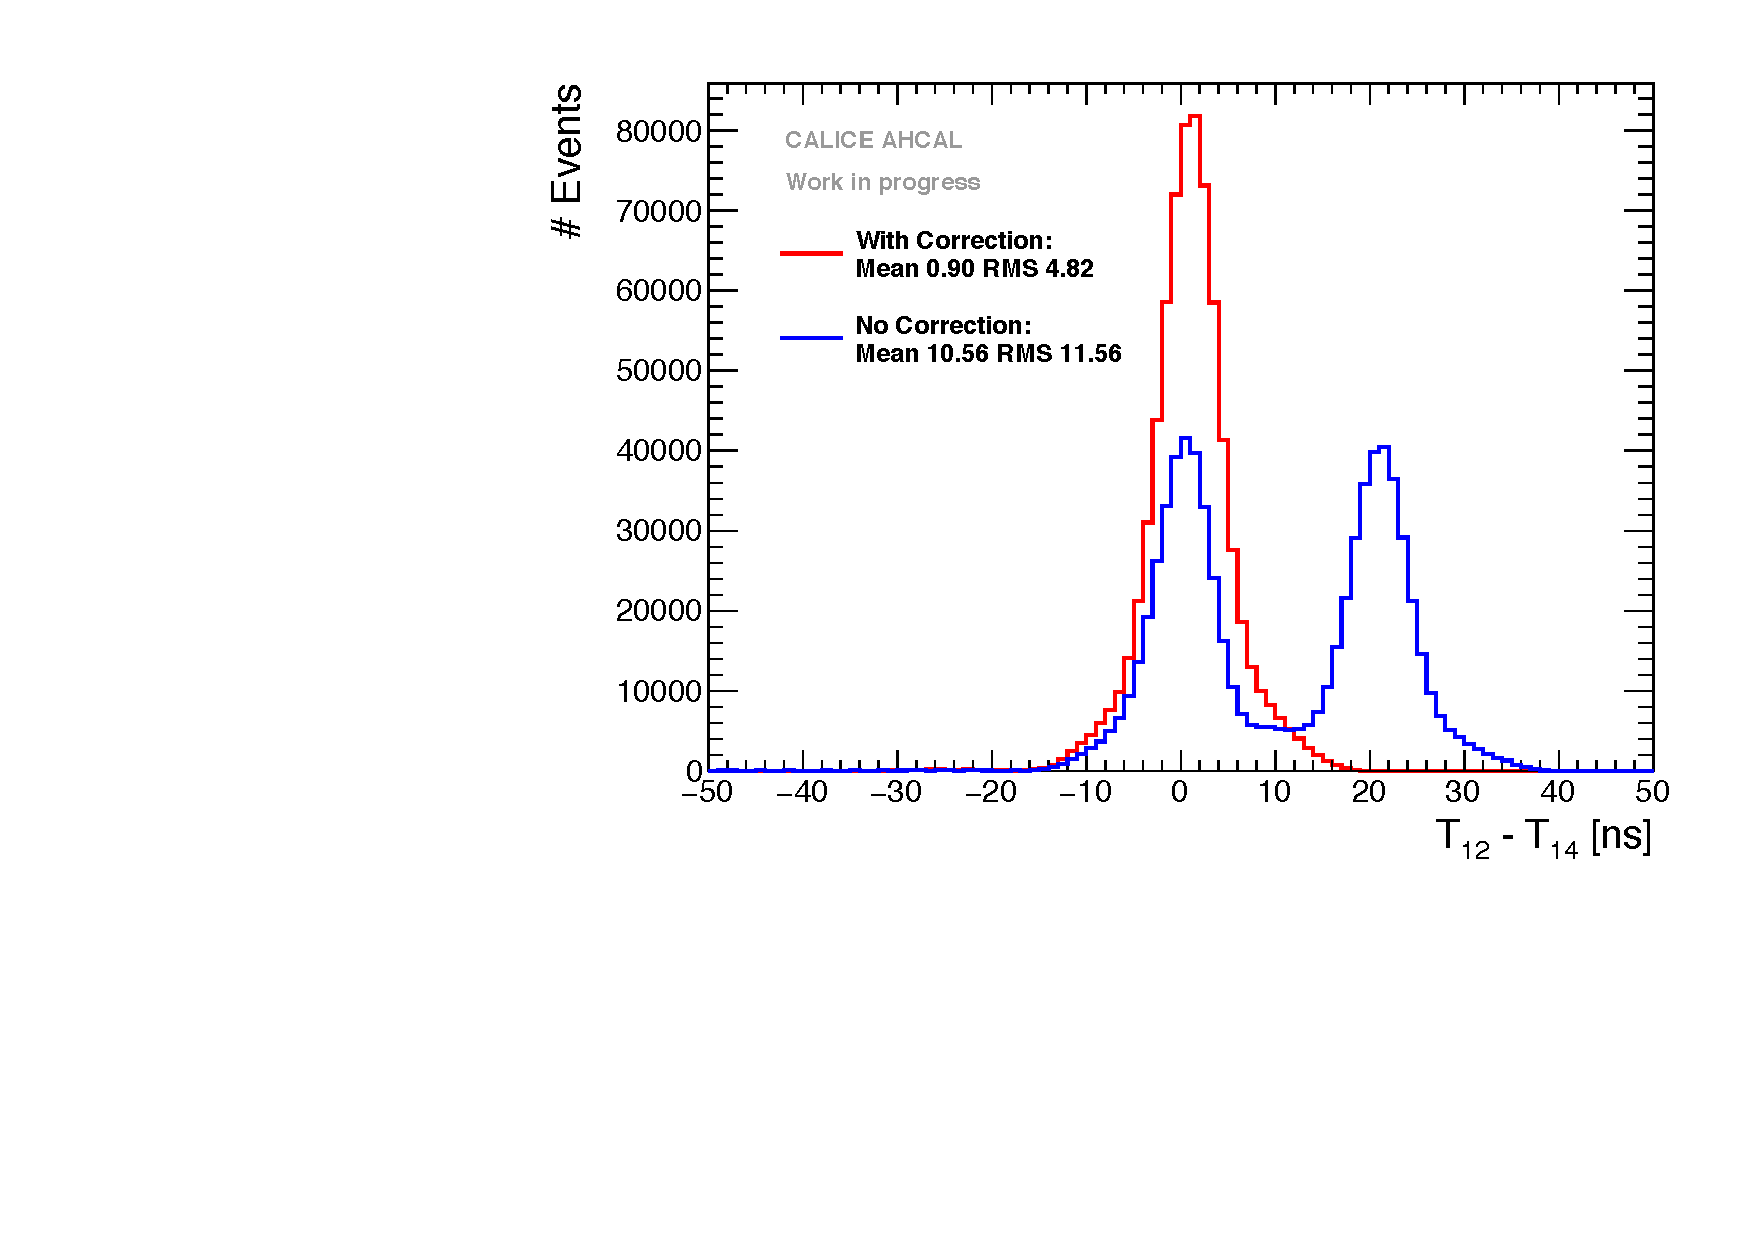
\includegraphics[width=0.6\textwidth]{fig/T0s/T0_Resolution_5.pdf}
\caption{Time difference between the trigger channels before and after correction for T$_{12}$ and T$_{14}$. The histogram in blue shows the difference between the channels before correction, the histogram in red shows the difference after correction. $\mu$ = 10.6 ns, RMS = 11.6 ns, $\mu_{corrected}$ = 0.9 ns, RMS$_{corrected}$ = 4.8 ns}
\label{fig:T0_Correction}
\end{center}
\end{figure}

In a next step, to reduce the uncertainty made on the time of the trigger, the time reference $T_{ref}$ is calculated using the mean of T$_{12}$, T$_{13}$ and T$_{14}$ and its associated error $\sigma_{ref}$ as shown in eq. \ref{eq:tref} \& \ref{eq:tref_err}. A cut of 4 ns is performed on $\sigma_{ref}$ to reject events with a too large error on the time of the trigger.
\begin{equation} \label{eq:tref}
\text{T}_{ref} = \frac{\text{T}_{12} + \text{T}_{13} + \text{T}_{14}}{3}
\end{equation}
\begin{equation} \label{eq:tref_err}
\sigma_{ref}^2 = \frac{ (\text{T}_{12} - \text{T}_{ref})^2 + (\text{T}_{13} - \text{T}_{ref})^2  + (\text{T}_{14} - \text{T}_{ref})^2 }{6}
\end{equation}

Since the absolute time between the passage of a muon and the trigger of a channel is not known due to cabling and the trigger electronics, the time offset relative to the trigger is determined from data. Muons are quasi-instantaneous particles thus the time of the first hit distribution for each channel, memory cells and BXID has to be shifted to \textit{t=0}. This shifting procedure takes into account the delay time of the trigger due to cabling and the NIM-logic as well as mis-calibrations in pedestals. Only memory-cells containing more than 100 events are considered. This offset is determined by iteration requiring at least 4 prompt hits i.e hits in the range from -20 to 20 ns of the event. In this way, 18338 individual offsets are extracted from data. A distribution of the extracted offsets using muon data can be seen in figure \ref{fig:offset_trigger_distribution}. The figure \ref{fig:BXID_offset} shows that individual offsets have to be extracted for each BXID as the correlation is chip-dependent and not the same for odd and even BXIDs.

\begin{figure}[htbp]
	\subfigure[Distribution of the offset used to correct for the trigger delay.\label{fig:offset_trigger_distribution}] {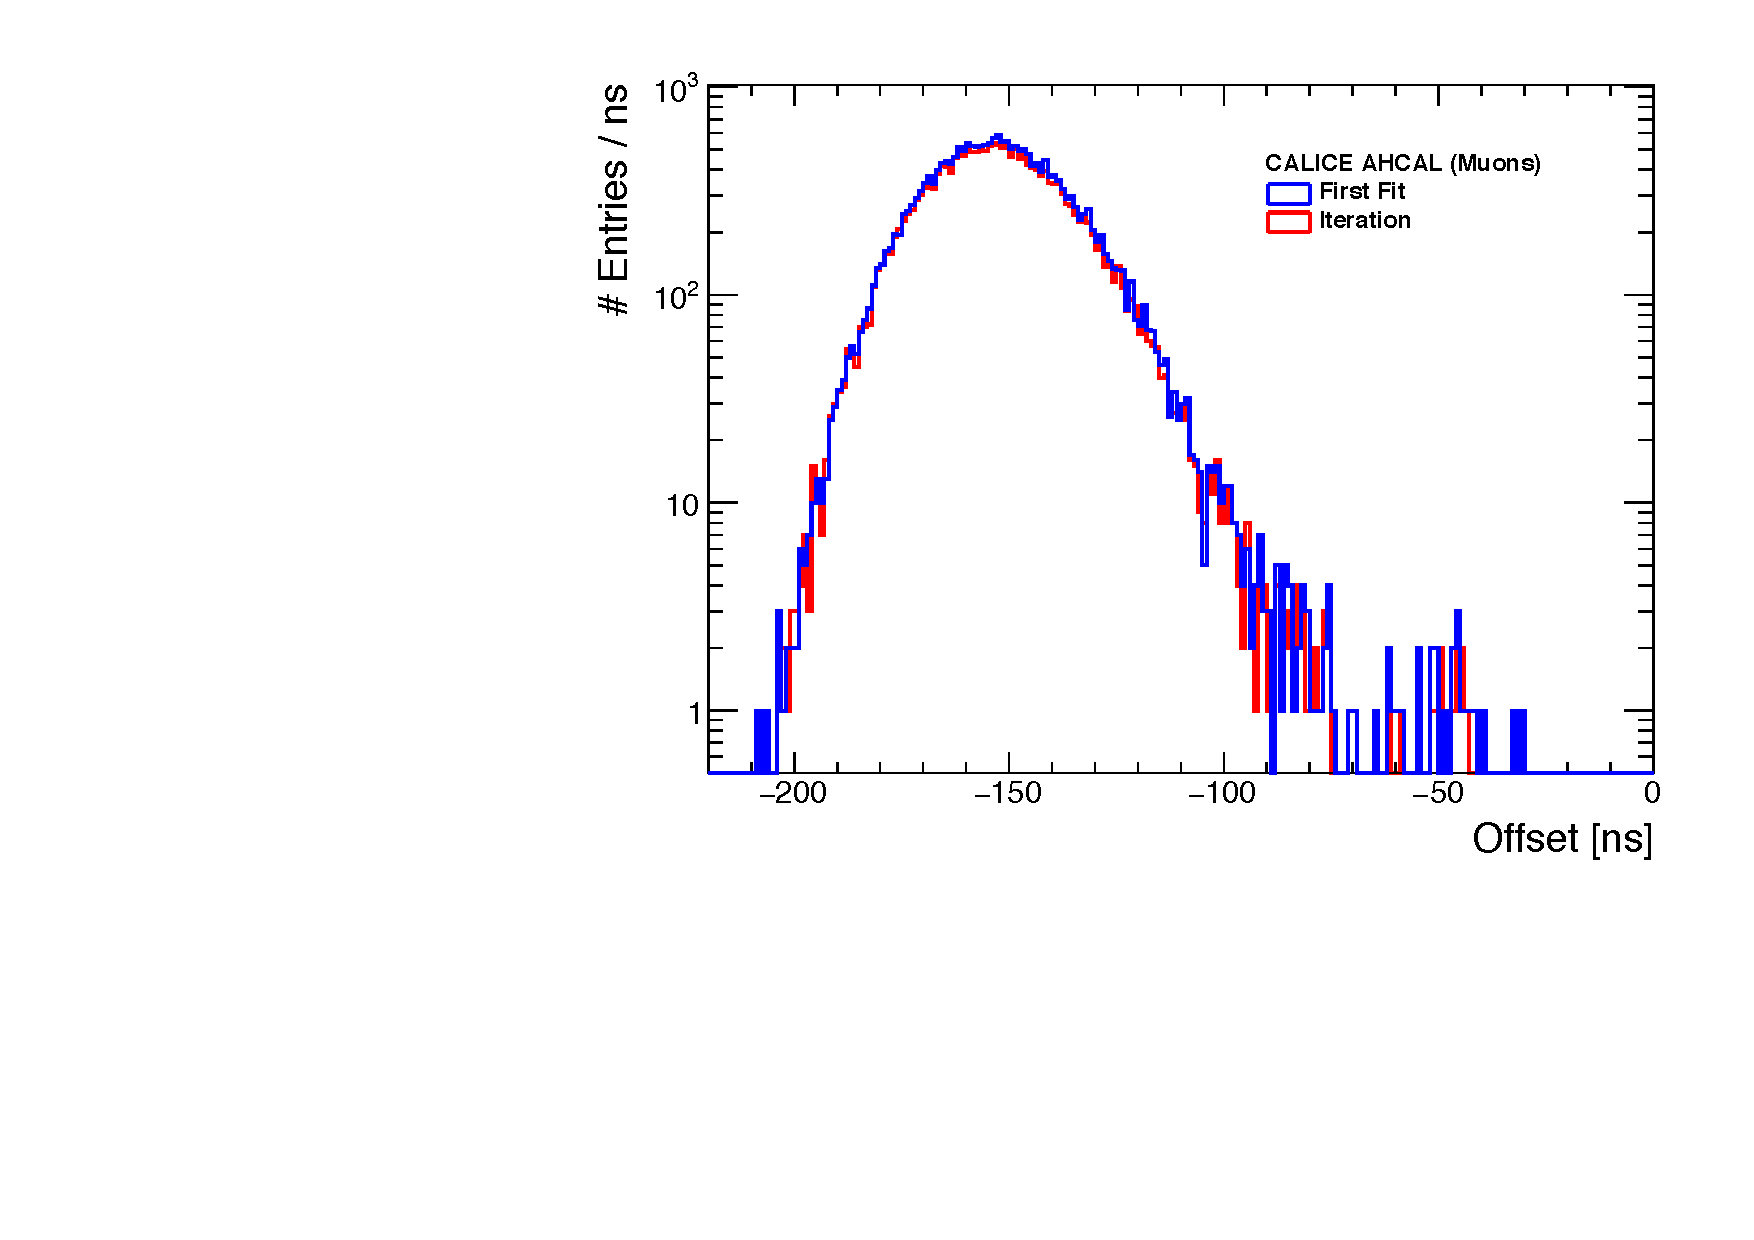
\includegraphics[width=0.5\textwidth]{fig/Muons/ExtractedOffsets.pdf}}\hfill
	\subfigure[Correlation between offsets extracted for even and odd BXID.\label{fig:BXID_offset}] {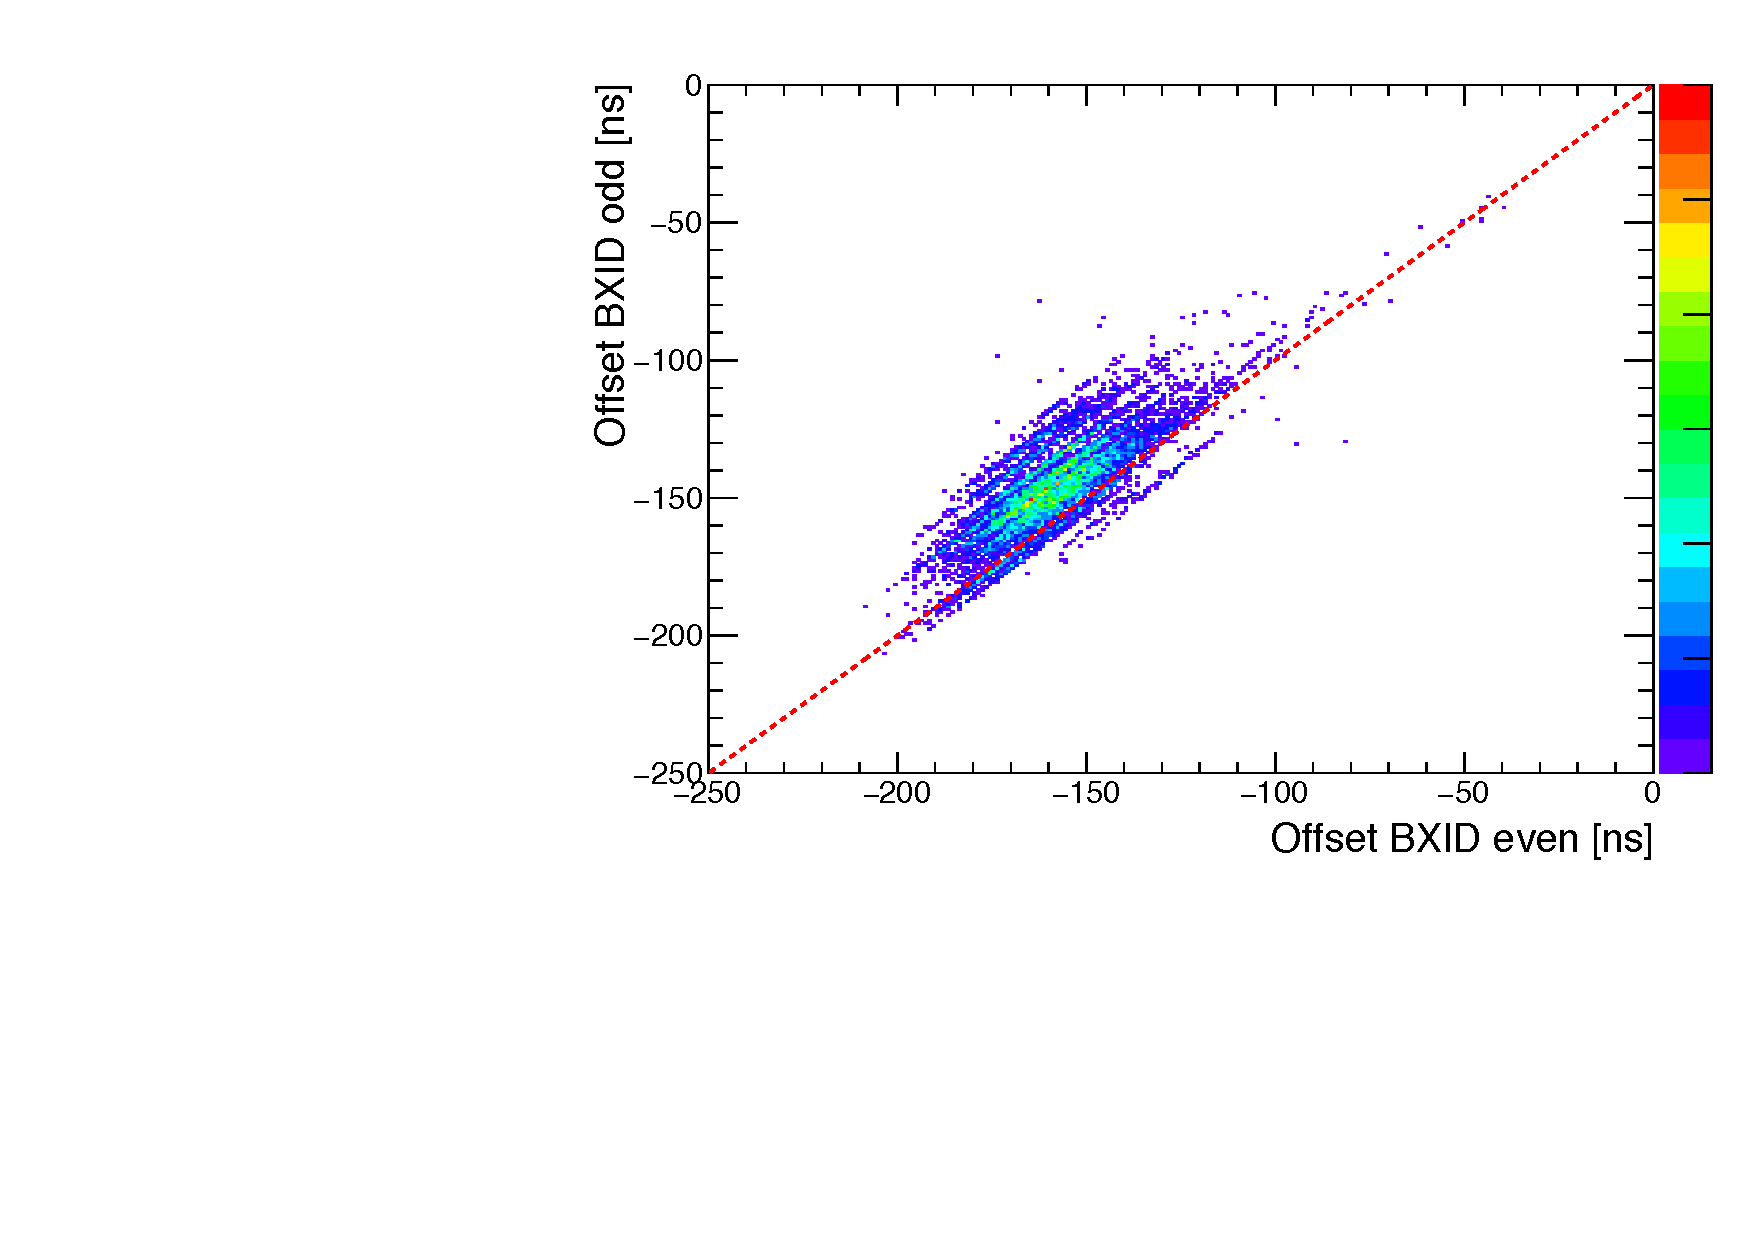
\includegraphics[width=0.5\textwidth]{fig/Muons/CorrelationOffsets_BXID.pdf}}\hfill
	\caption[]{\textbf{a}: Extracted offset used to correct for the trigger delay signal. The mean delay of the trigger is $\sim$150 ns. \textbf{b}: Correlation between offsets extracted for BXID even and odd.}
\end{figure}

\subsubsection{Time of the first hit distribution}
After the selection, the time of the first hit (T$_{fH}$) can be obtained by plotting the distribution of T$_{chn}$ - T$_{ref}$ as shown in figure \ref{fig:timing_nocorrection}. The combined time resolution (RMS) shown in figure \ref{fig:reso_nocorrection} obtained by combining all layers is around 5.65 ns by just applying the time calibration on the data. Some improvements are possible as described in the subsections \ref{subsec:lin_corr} and \ref{subsec:timewalk}. The discrepancy observed for the layer 11 is most likely due to an electronic problem in the TDC voltage ramp of the chips on that layer.

\begin{figure}[htbp]
	\subfigure[Timing for all layers in the AHCAL.\label{fig:timing_nocorrection}] {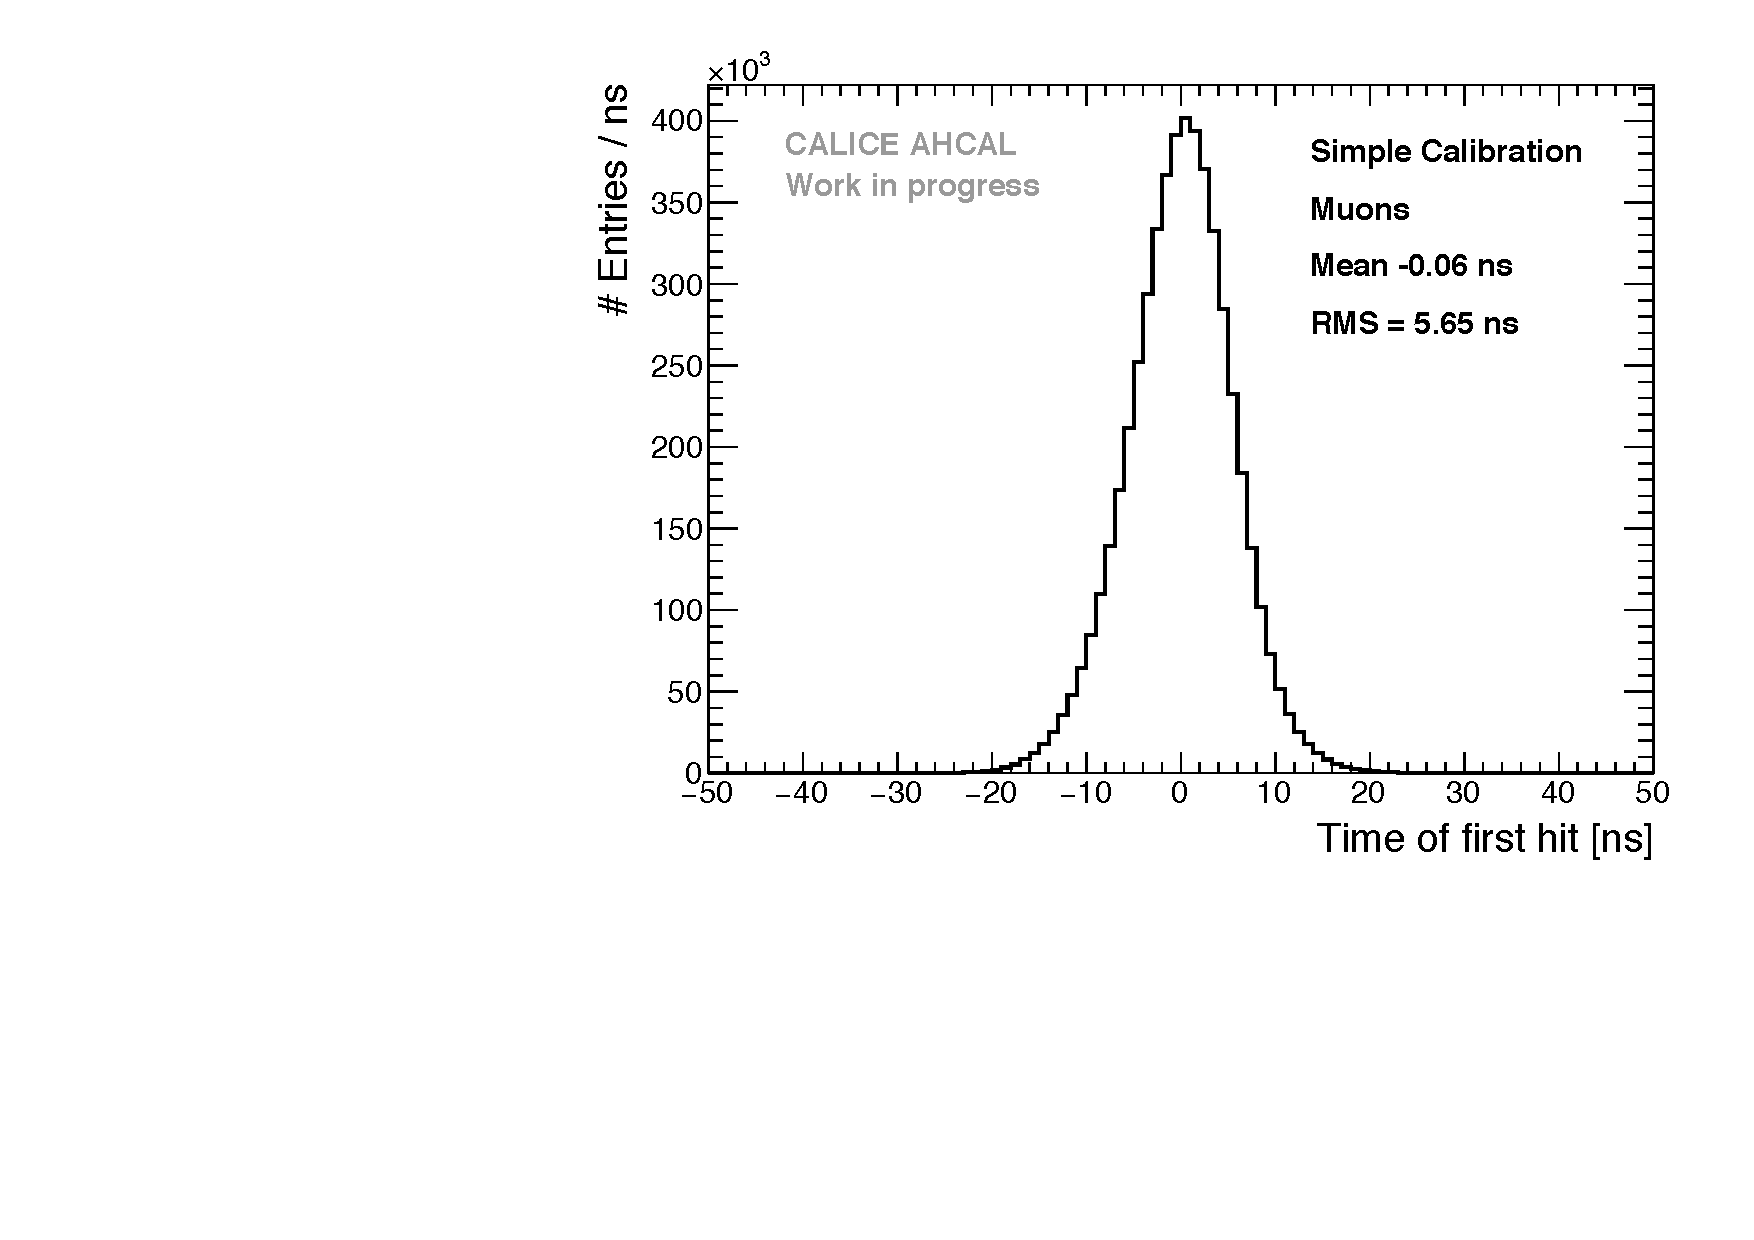
\includegraphics[width=0.5\textwidth]{fig/Muons/Timing_AHCAL_noCorrections.pdf}}\hfill
	\subfigure[Extracted resolution for all layers in the AHCAL.\label{fig:reso_nocorrection}] {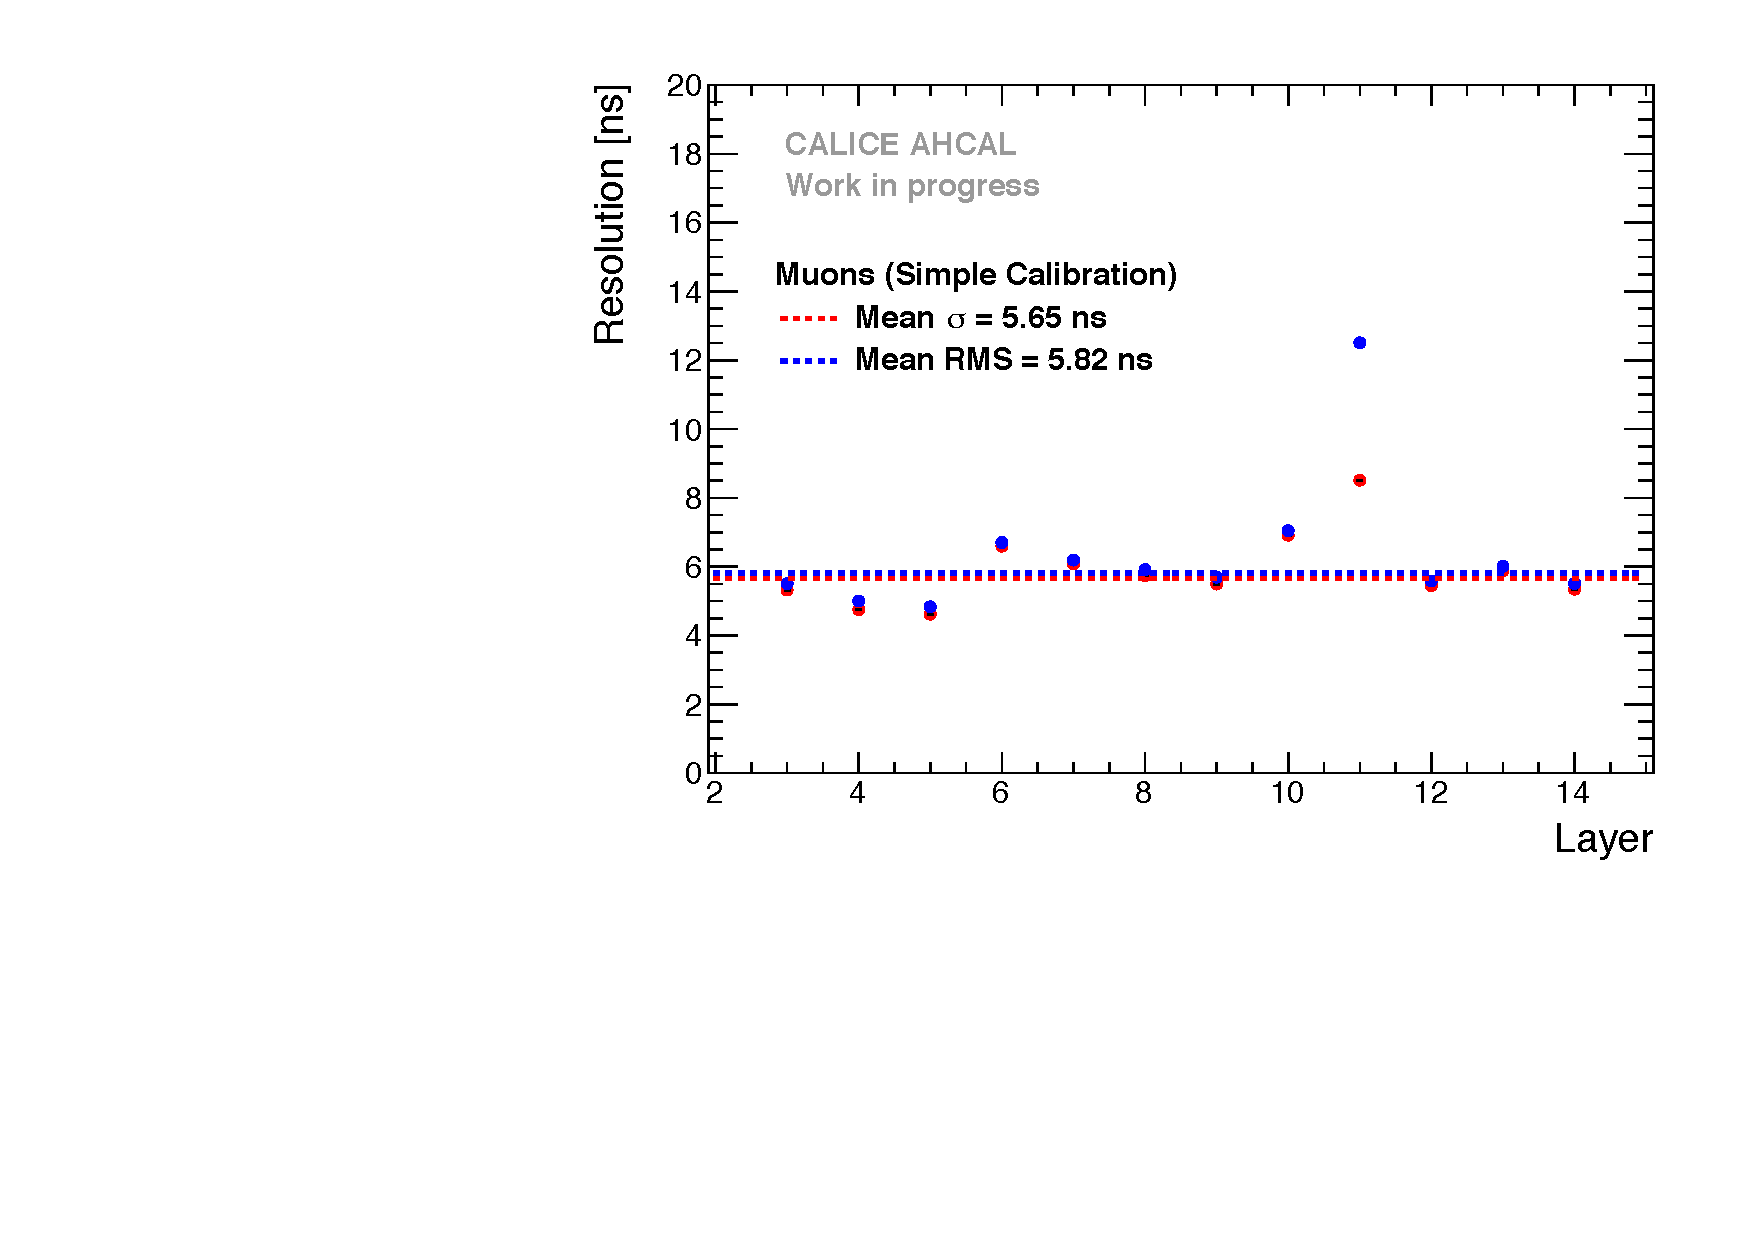
\includegraphics[width=0.5\textwidth]{fig/Muons/ResolutionPerModule_noCorrections.pdf}}\hfill
\caption[]{\textbf{a}: Time of the first hit distribution of the AHCAL after the first part of the calibration. $\mu$ = -0.06 ns , RMS = 5.65 ns. The distribution is clearly asymmetric. \textbf{b}: Time resolution for all layers in the AHCAL. The mean RMS is 5.65 ns.}
\end{figure}

\subsection{Corrections applied to data}
\subsubsection{Ramp non-linearity correction}
\label{subsec:lin_corr}

The calibration relies on the linearity of the TDC voltage ramp in the SPIROC2b by measuring the minimum and maximum of the ramp and interpolating assuming a linear ramp. This assumption is not entirely reliable as described in \cite{OskarSSP, EldwanSSP}. For this, a correction of the non-linearity has to be applied. By simply looking at the time of the first hit (T$_{fH}$) for each chip and BXID versus the TDC value of the hit, the shape of the graph would indicate how reliable is the assumption. Indeed if the ramp would be perfectly linear, one would obtain a flat graph. A quadratic fit is performed for each chip and BXID in order to correct for the non-linearity of the ramp as shown in figure \ref{fig:LinCorr}. A check has been performed on the quality of the correction, seen in figure \ref{fig:LinCorr_2}. The non-linearity correction results in an improvement on the timing resolution (RMS) of the AHCAL of $\sim$5.1\% (5.36 ns) as shown in figure \ref{fig:timing_lincorrection}.

\begin{figure}[htbp]
	\subfigure[Quadratic fit of chip 146 (BXID even) on layer 09.\label{fig:LinCorr}]{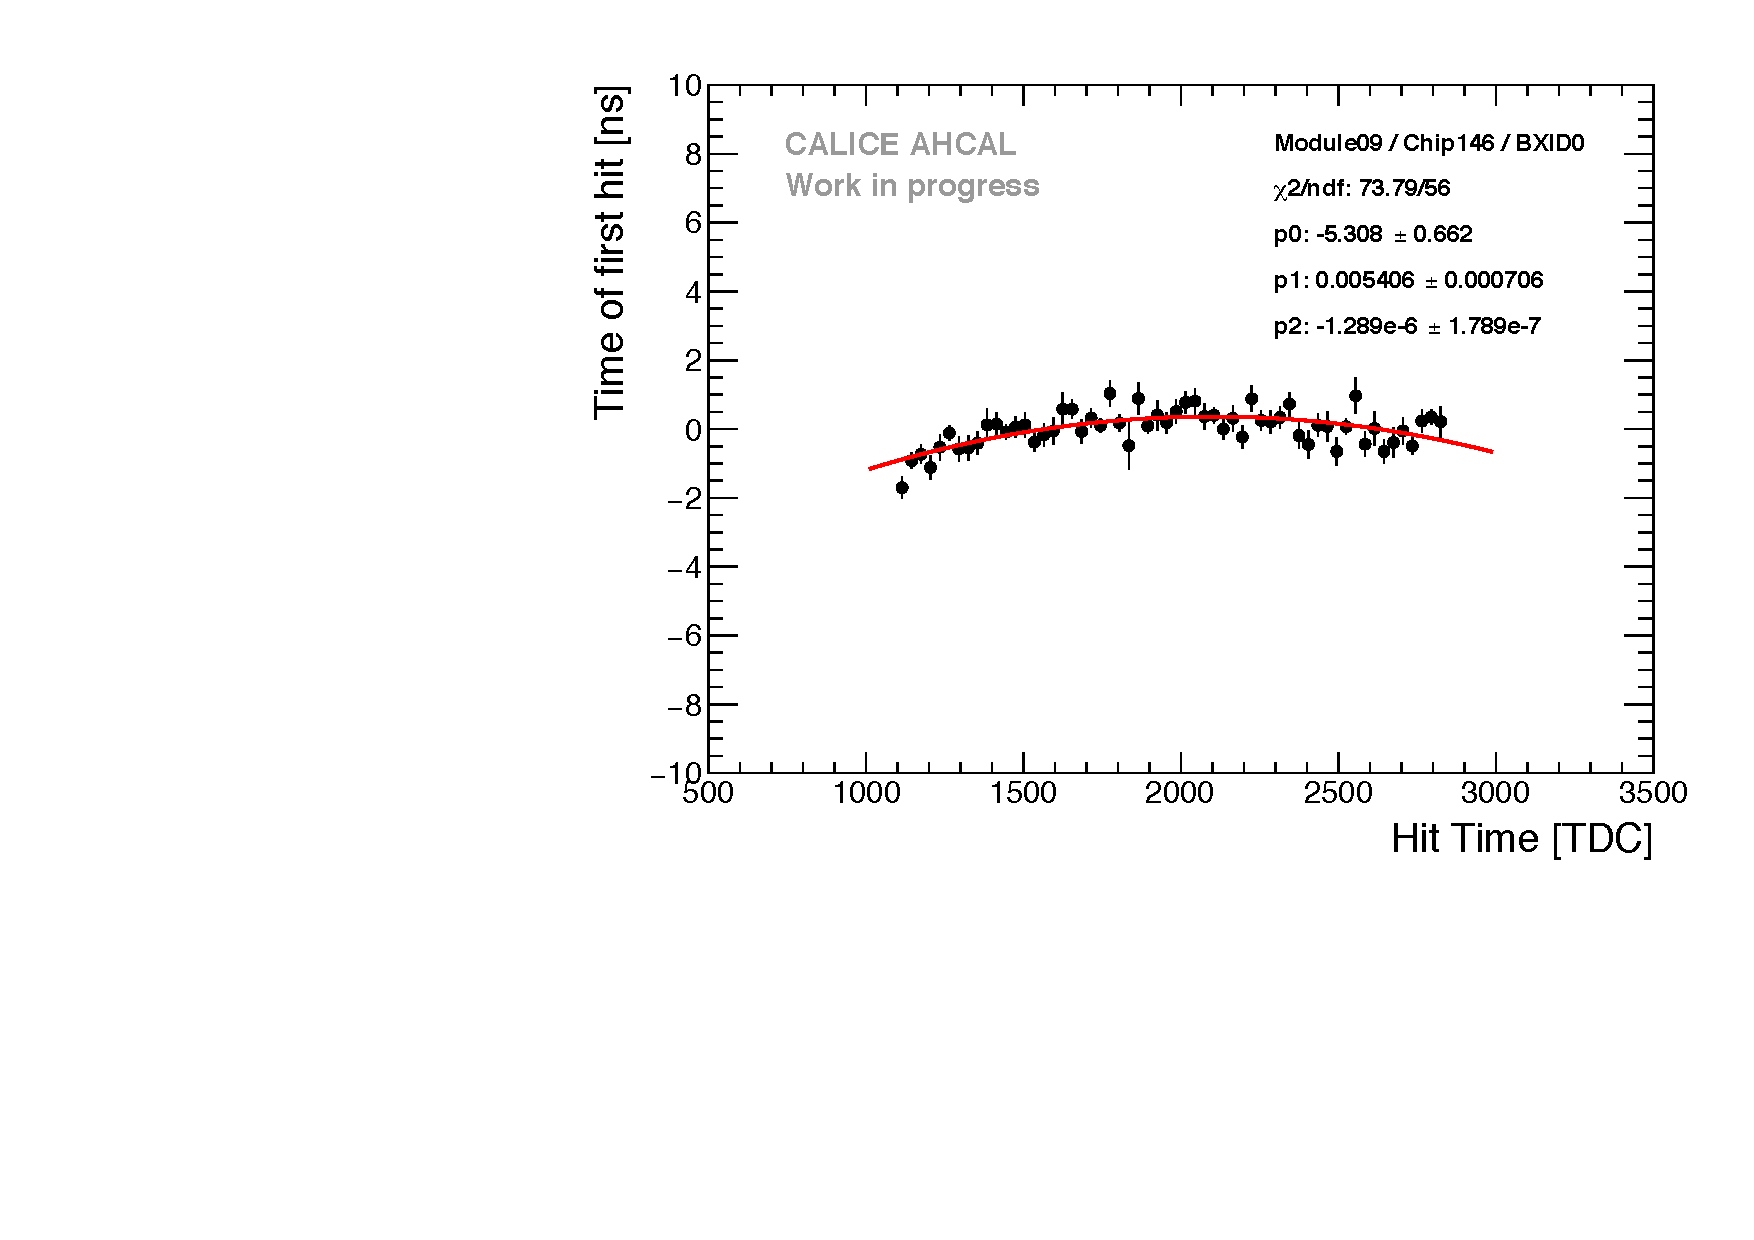
\includegraphics[width=0.5\textwidth]{fig/Muons/LinearityCorrection_Module09_Chip146_BXID0.pdf}}\hfill
	\subfigure[Profile for chip 146 on layer 09 after the non-linearity correction of the ramp.\label{fig:LinCorr_2}]{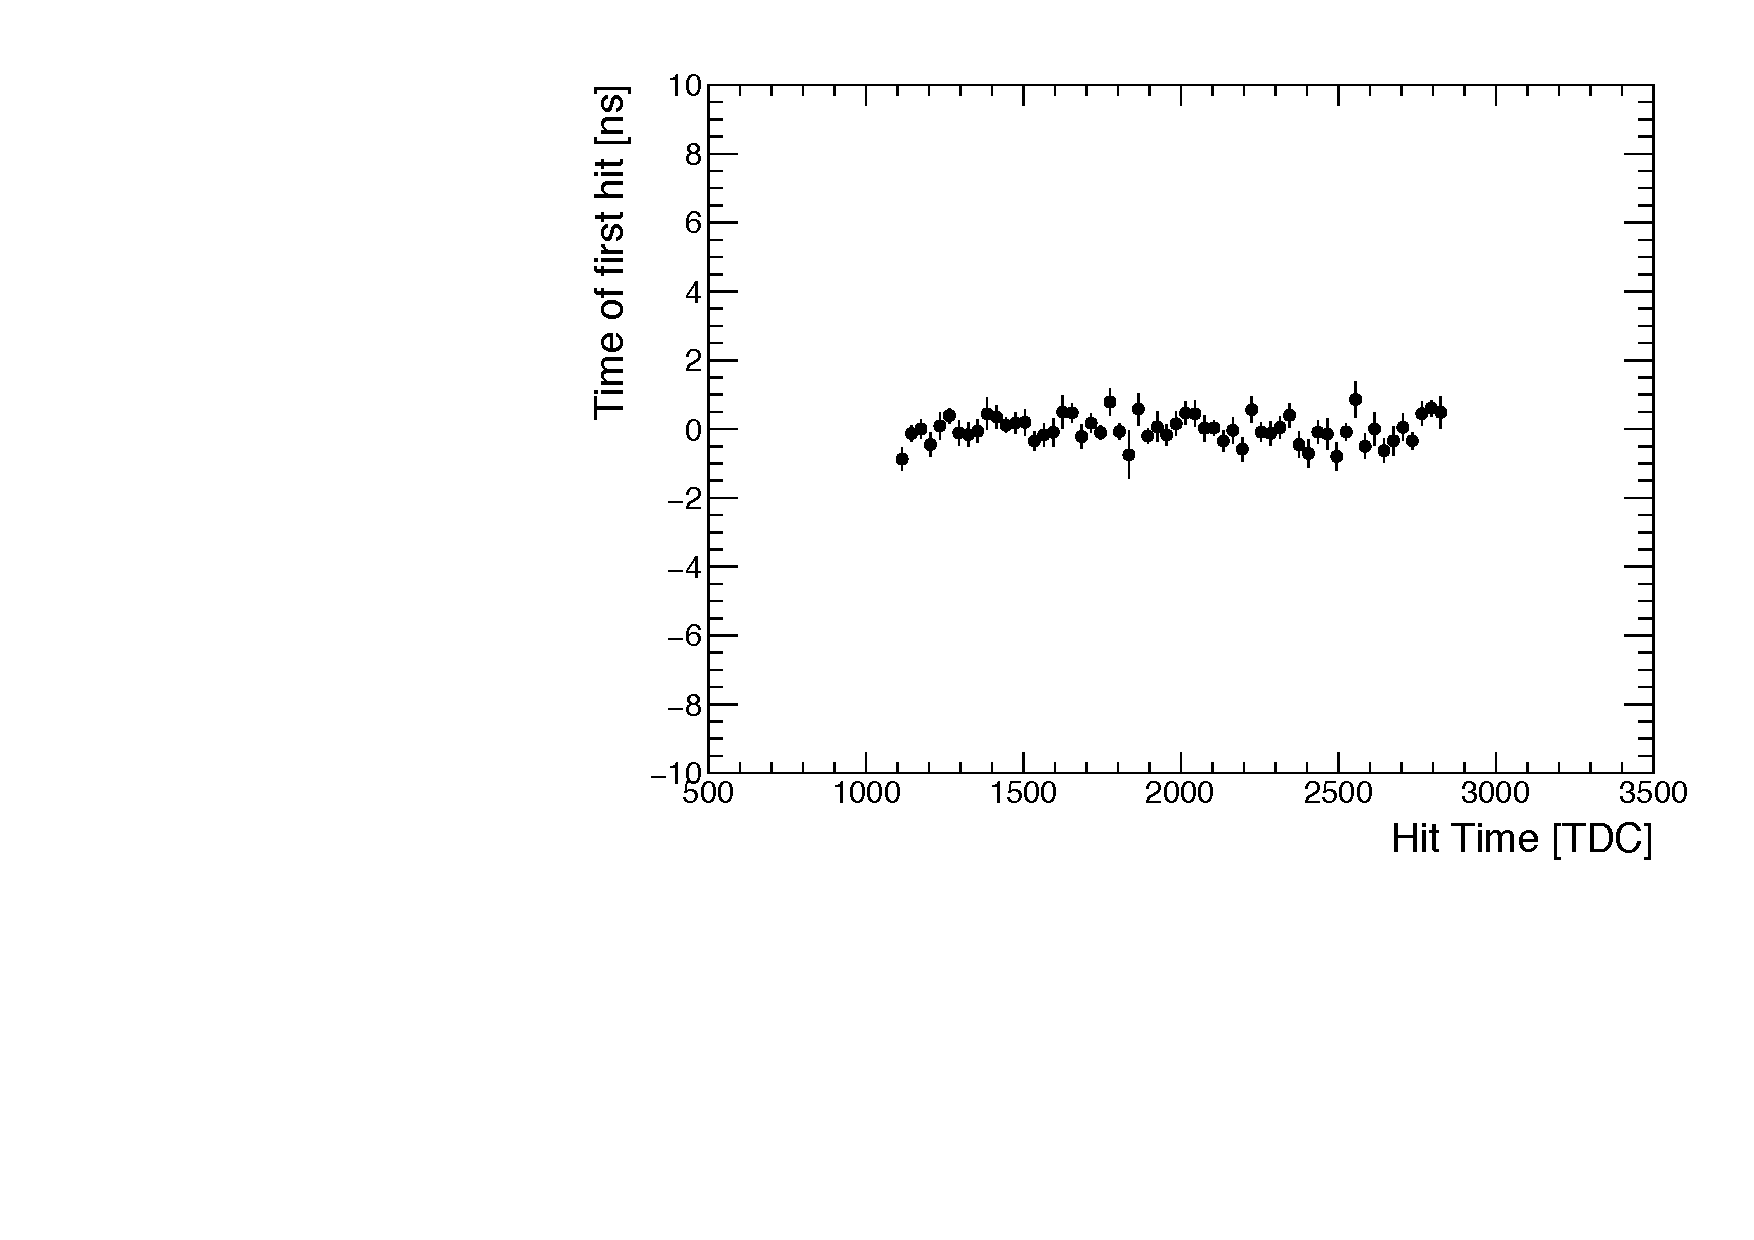
\includegraphics[width=0.5\textwidth]{fig/Muons/LinearityCorrection_Module09_Chip146_BXID0_Corrected.pdf}}
	\caption[]{\textbf{a}: The $\chi^2$ of the fit is 1.29. \textbf{b}: The correction parameter are applied then on the data to cross-check the quality of the correction. One can see that the curve flattens with the correction applied.}
\end{figure}

\begin{figure}[htbp]
	\subfigure[Timing for all layers in the AHCAL.\label{fig:timing_lincorrection}] {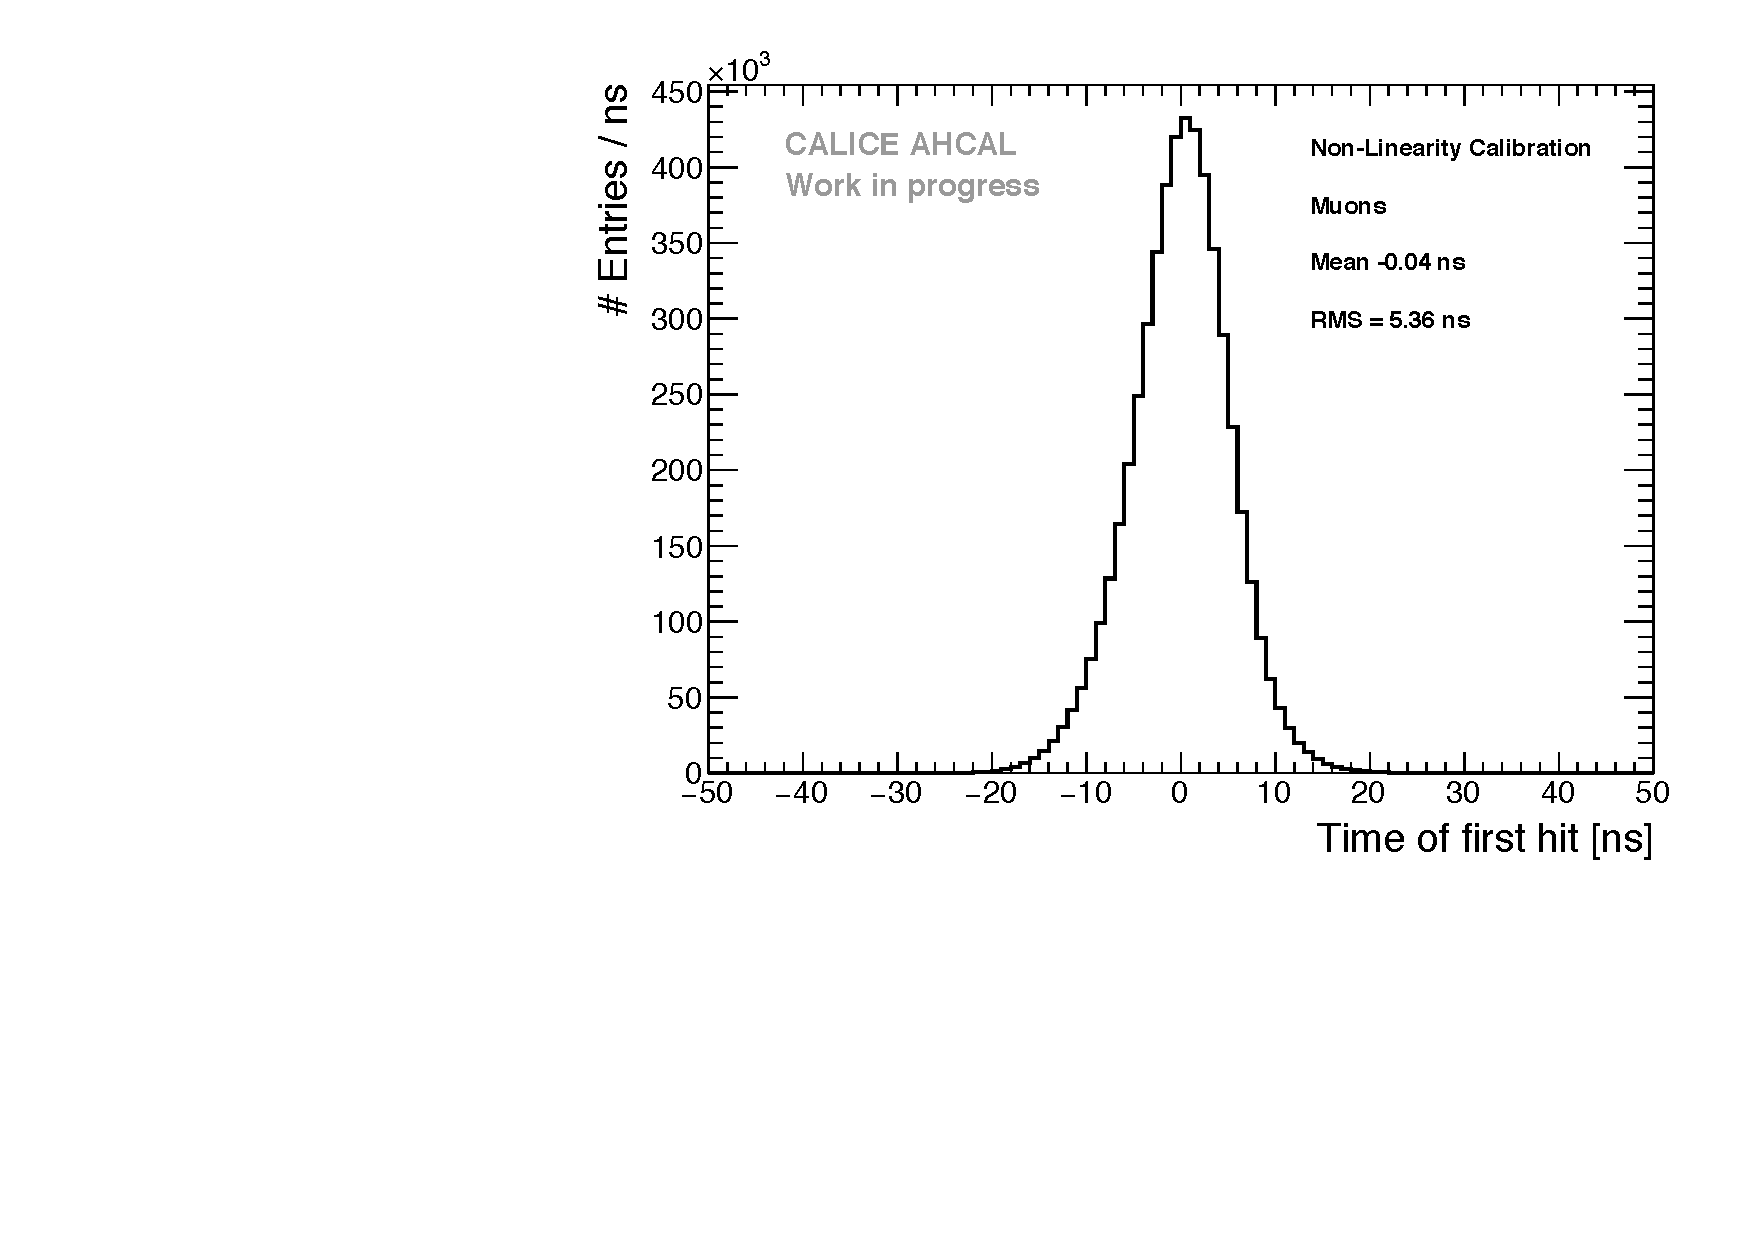
\includegraphics[width=0.5\textwidth]{fig/Muons/Timing_AHCAL_LinCorrection.pdf}}\hfill
	\subfigure[Extracted resolution for all layers in the AHCAL.\label{fig:reso_lincorrection}] {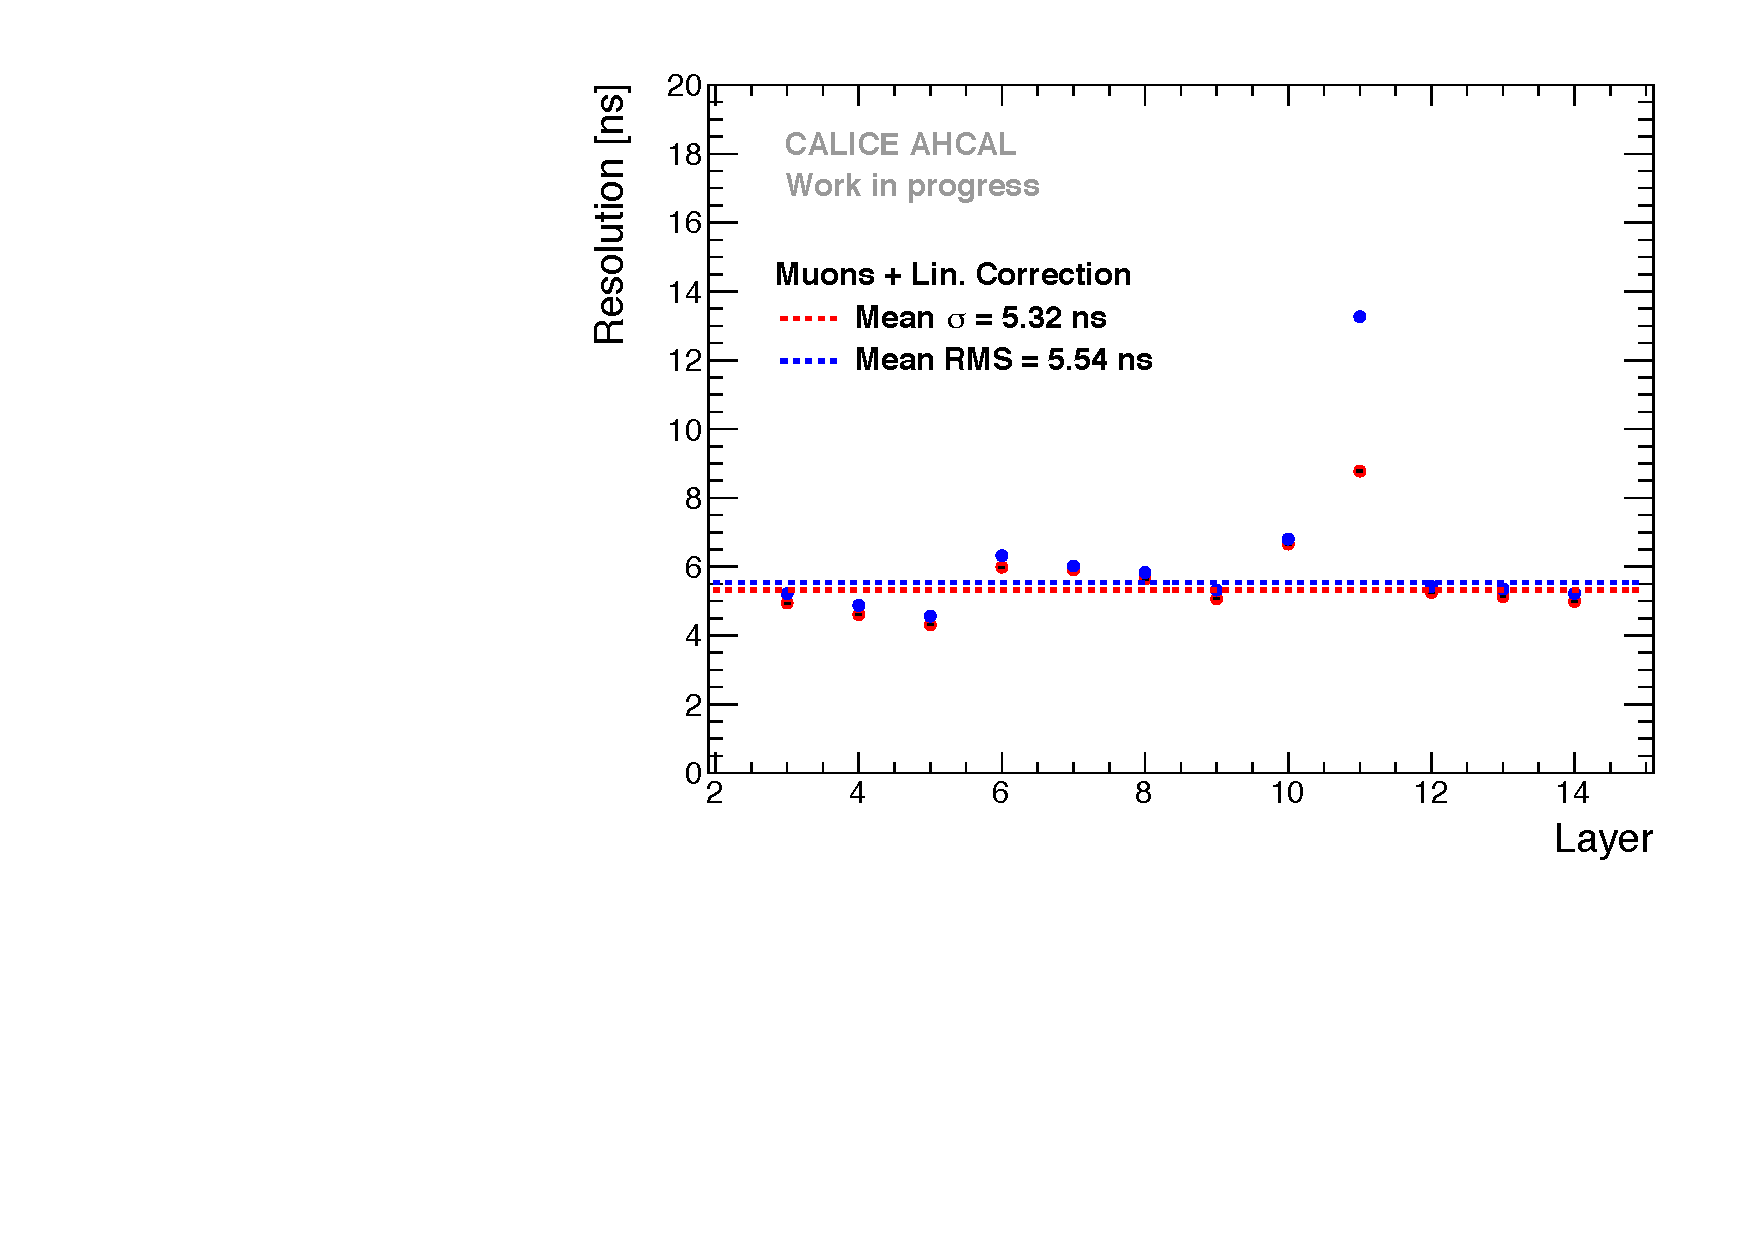
\includegraphics[width=0.5\textwidth]{fig/Muons/ResolutionPerModule_LinCorrection.pdf}}\hfill
\caption[]{\textbf{a}: Time of the first hit distribution of the AHCAL after the non-linearity correction. $\mu$ = -0.04 ns , RMS = 5.36 ns. \textbf{b}: Time resolution for all layers in the AHCAL. The mean RMS is 5.54 ns.}
\end{figure}

\subsubsection{Time Walk correction}
\label{subsec:timewalk}

The time-walk effect is due to the presence of a threshold that induces a time shift between a small amplitude signal and a high amplitude signal. Small amplitude signals will systematically trigger at a later time than high amplitude signals. A correction can be applied on the data by looking at the time of the first hit versus the amplitude of the hit. This might be particularly important for late neutrons signals that generally deposit very little energy in the calorimeter. The correction is assumed to be the same for all the chips, independent of the position of the threshold of each chip, as hits are cut at 0.5 MIP and most of the chips were having the threshold set-up well below 0.5 MIP. An exponential fit of the form $\text{A} \times e^{-\lambda{}x} + \text{B}$ is performed on the data to extract the parameters needed to correct the time walk effect as shown on figure \ref{fig:time_walk}. The residuals after correction are in the order of few hundreds of picoseconds as seen in figure \ref{fig:time_walk_corr}.

\begin{figure}[htbp]
	\subfigure[Profile of the time of first hit as function of the hit energy.\label{fig:time_walk}] {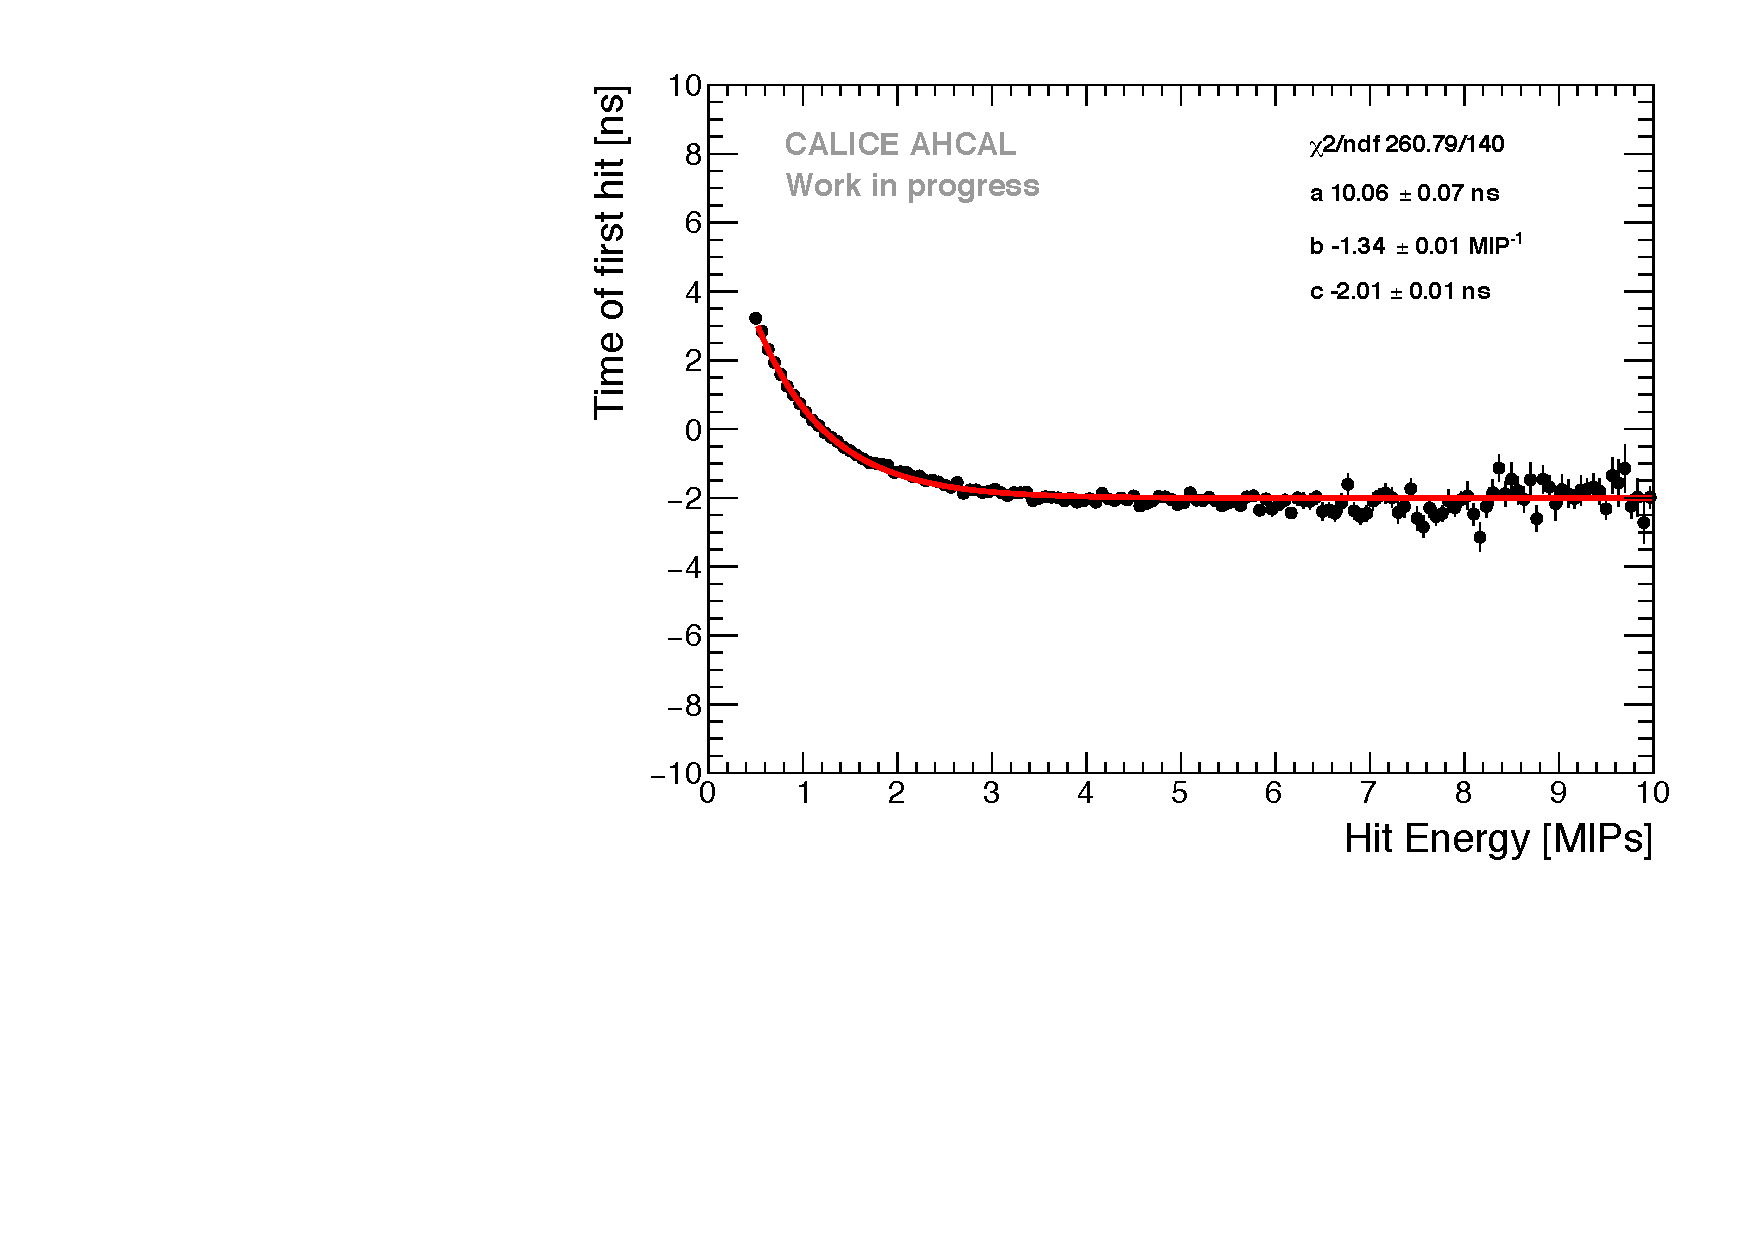
\includegraphics[width=0.5\textwidth]{fig/Muons/TimeWalkProfile.pdf}}\hfill
	\subfigure[Same profile after time-walk correction.\label{fig:time_walk_corr}] {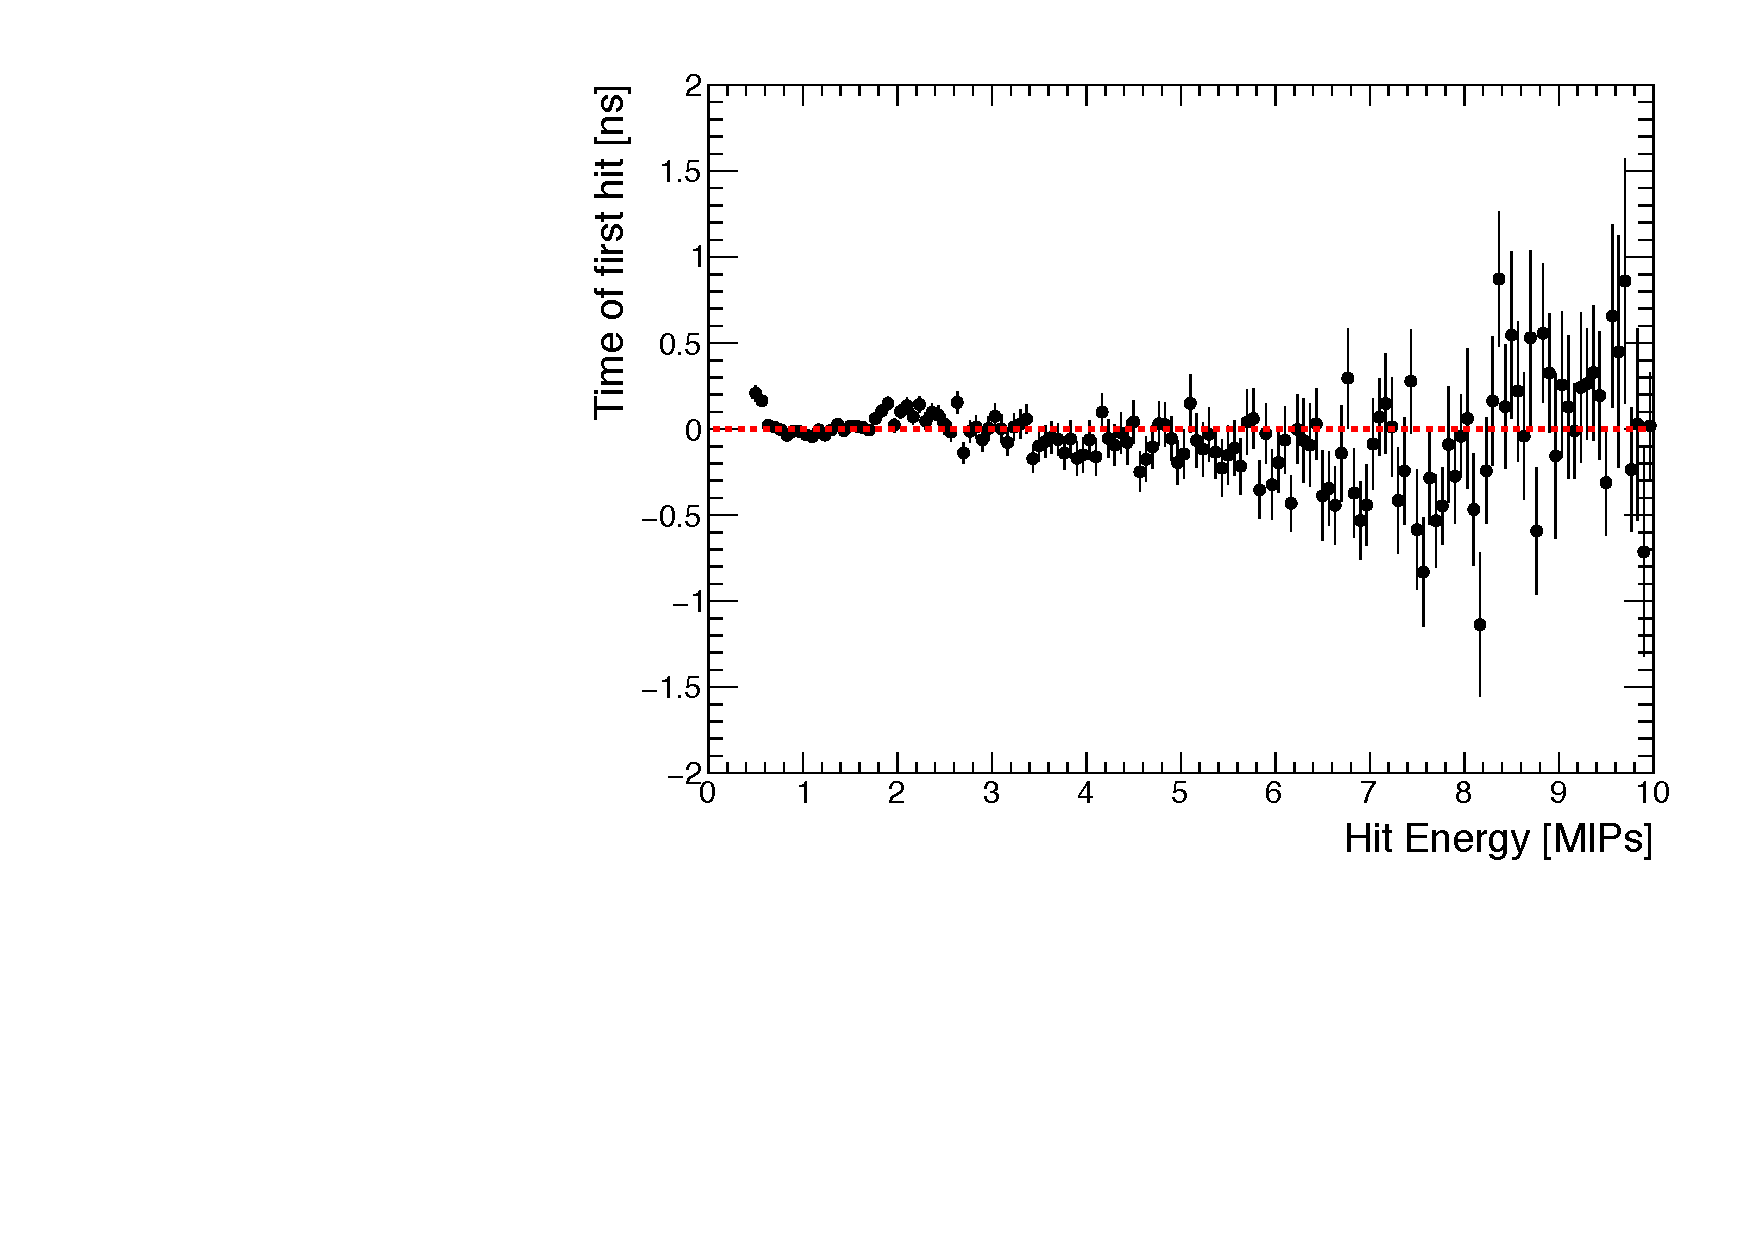
\includegraphics[width=0.5\textwidth]{fig/Muons/TimeWalkProfile_Correction.pdf}}
	\caption[]{\textbf{a}: Time-walk correction extracted from data. A = 10.06 $\pm$ 0.07, $\lambda$ = -1.34 $\pm$ 0.01, B = -2.01 $\pm$ 0.01. A difference up to 6 ns is seen between small and large amplitudes. \textbf{b}: Time-walk profile after correction showing a spread of less than 1 ns.}
\end{figure}

\subsubsection{Time of first hit for muons}
\label{subsec:Muon_final}

After the time-walk correction, an improvement of $\sim$3\% can be achieved on the time resolution of the AHCAL (RMS 5.20 ns) as shown in figure \ref{fig:timing_muons}. The figure \ref{fig:timing_reso_all_muons} shows the time resolution obtained in the complete AHCAL. The obtained time resolution is around 5 ns. The distribution is still asymmetric, it is most likely coming from the non-linearity of the TDC ramp of the trigger reference as no external time is available to correct for it. This is taken into account in the simulation by parametrising the time distribution with a double Gaussian function. The number of events identified later than 5$\sigma$ ($\sim$25 ns) is around 1.22\% giving us a good assessment of the noise suppression for muons.

\begin{figure}[htbp]
	\subfigure[Time of the first hit distribution of the AHCAL after all corrections.\label{fig:timing_muons}] {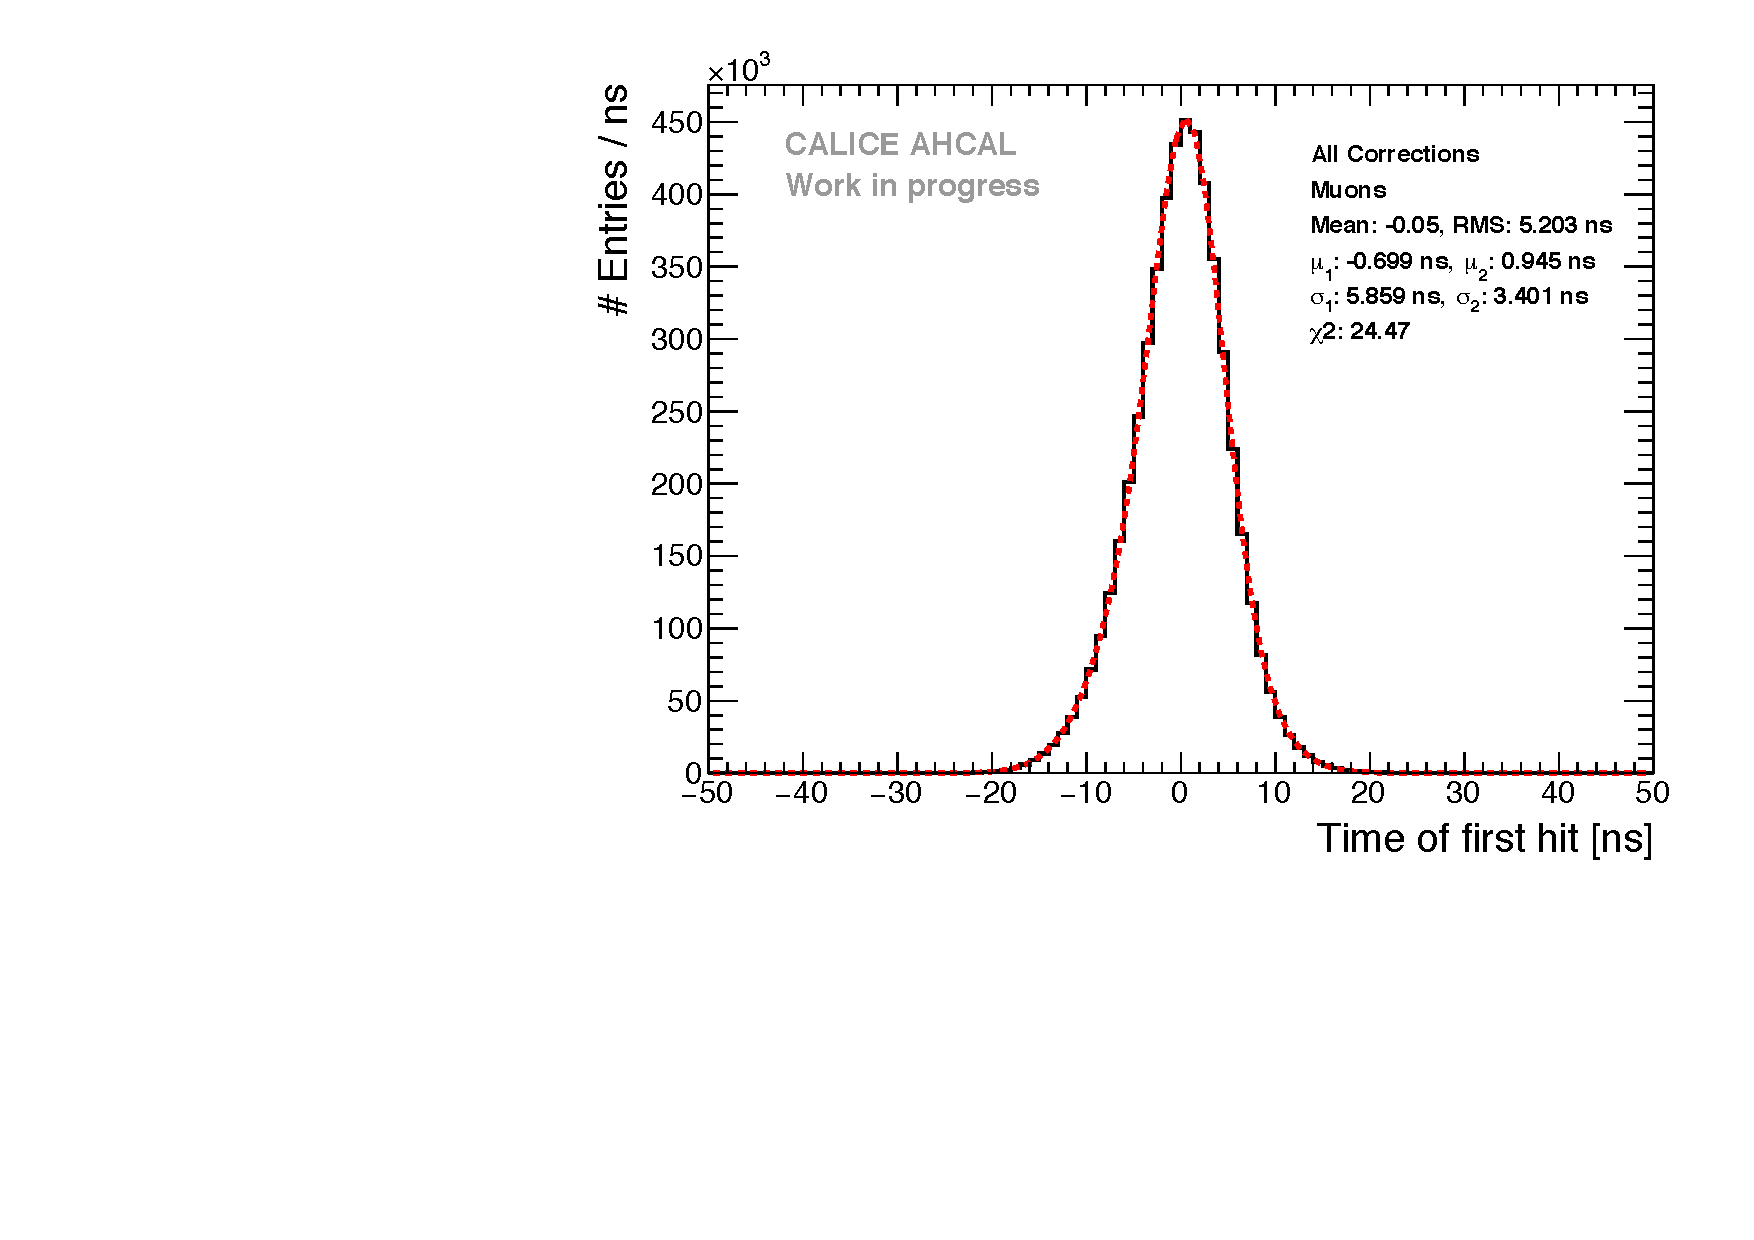
\includegraphics[width=0.5\textwidth]{fig/Muons/Timing_AllLayers.pdf}}
	\subfigure[Time resolution obtained for each AHCAL layers.\label{fig:timing_reso_all_muons}] {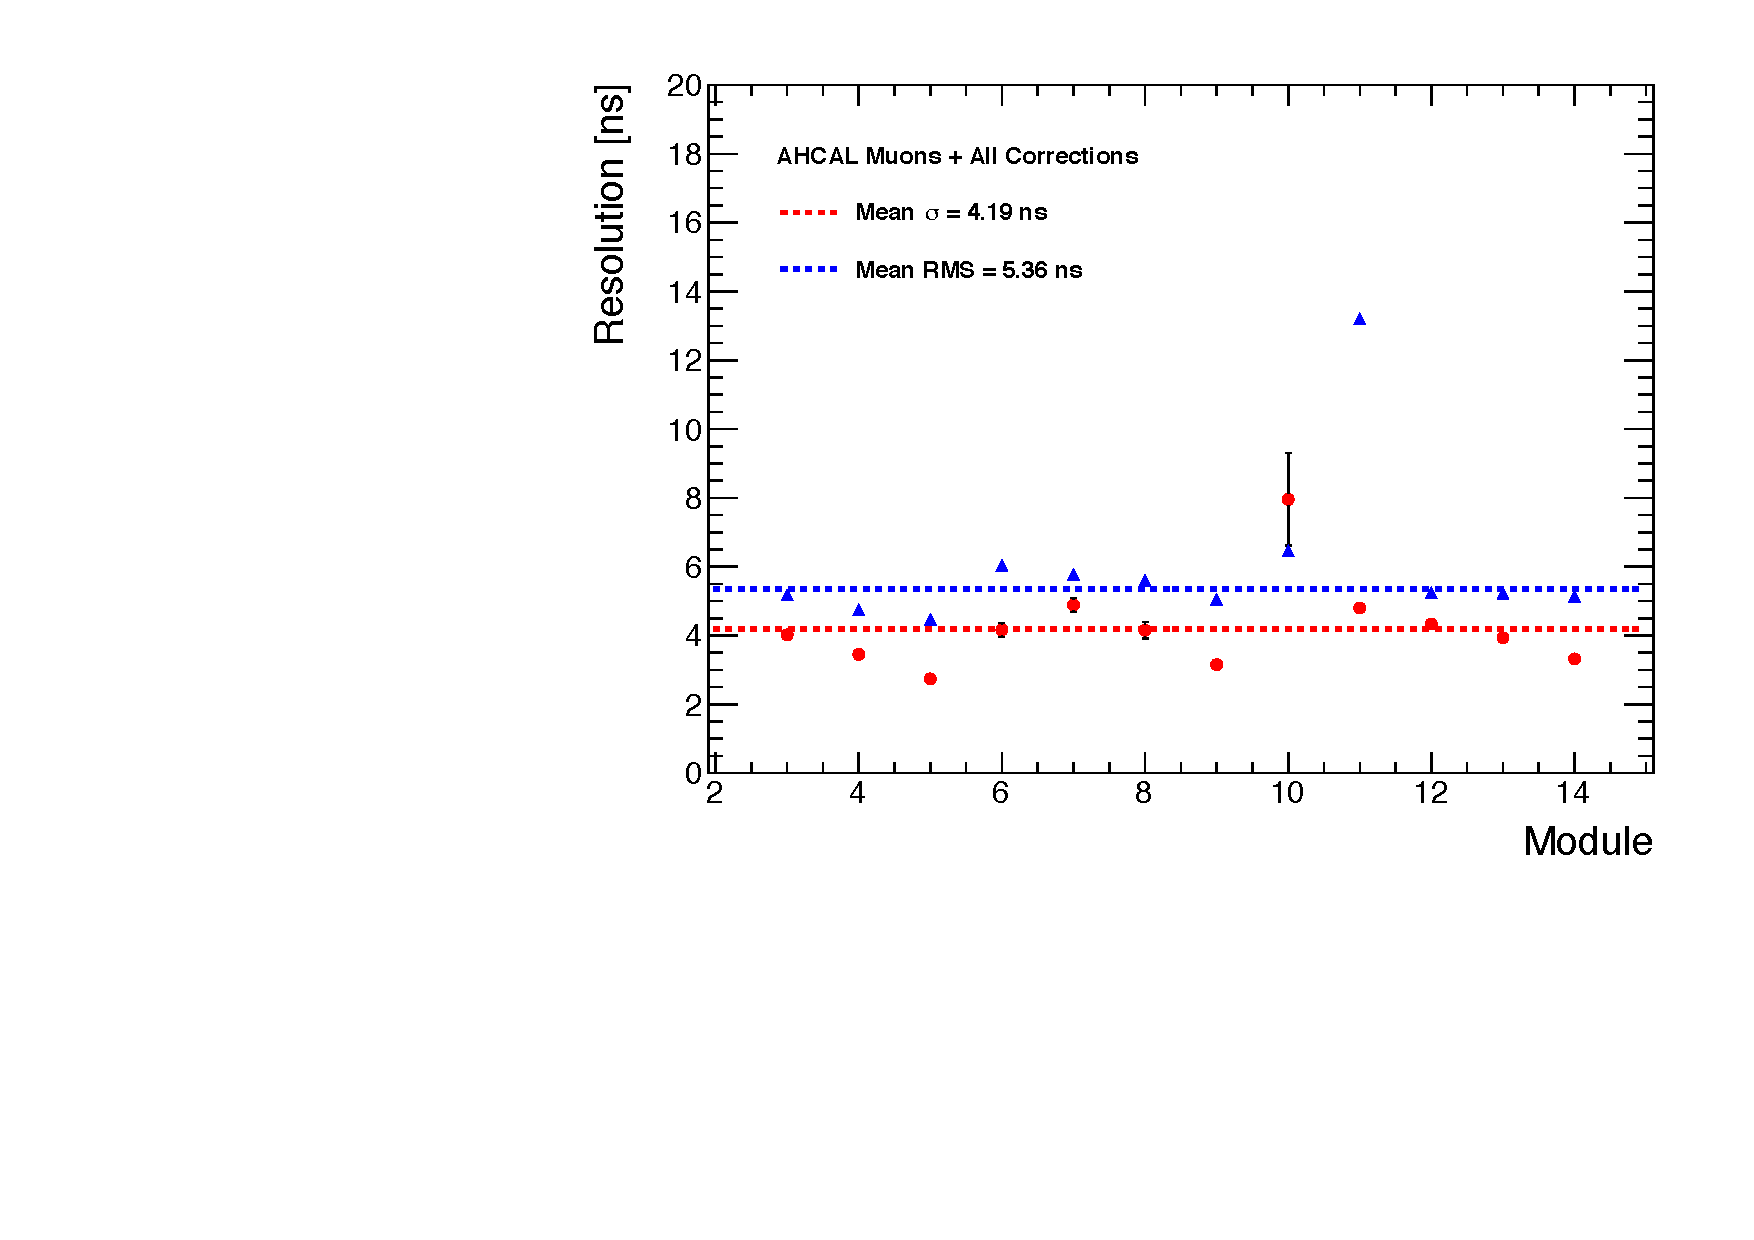
\includegraphics[width=0.5\textwidth]{fig/Muons/ResolutionPerModule_AllCorrection.pdf}}\hfill
	\caption[]{\textbf{a}: Time of the first hit for muons after all corrections. \textbf{b}: Time resolution obtained for each layer in the AHCAL. Mean RMS = 5.35 ns.}
\end{figure}

\subsection{Cross-check of the calibration with electrons}
\label{subsec:validation}

In order to validate the calibration, an electron sample is taken. Electromagnetic showers are quasi-instantaneous and perfect to cross-check the time calibration procedure. The selection applied to the data sample is described in subsection \ref{subsec:elec_sel}. The same calibration constants and correction constants are applied to the data except that an additional offset from the trigger signal has to be corrected for. The additional offset is expected to be small as the trigger configuration is very similar to the one for muons. The offset is in the order of 10 ns which is consistent with the changes in trigger configuration. The time of the first hit distribution is shown in figure \ref{fig:Timing_electrons}. The time distribution presents a large tail to the right and is much wider than for muons. This gives a hint that an effect is present in electron data but not in muon data. The difference seen could be related to the fact that in electromagnetic showers, the number of hits is much higher as well as the energy deposited in a single cell can be over hundreds MIP.

\begin{figure}[htbp]
\begin{center}
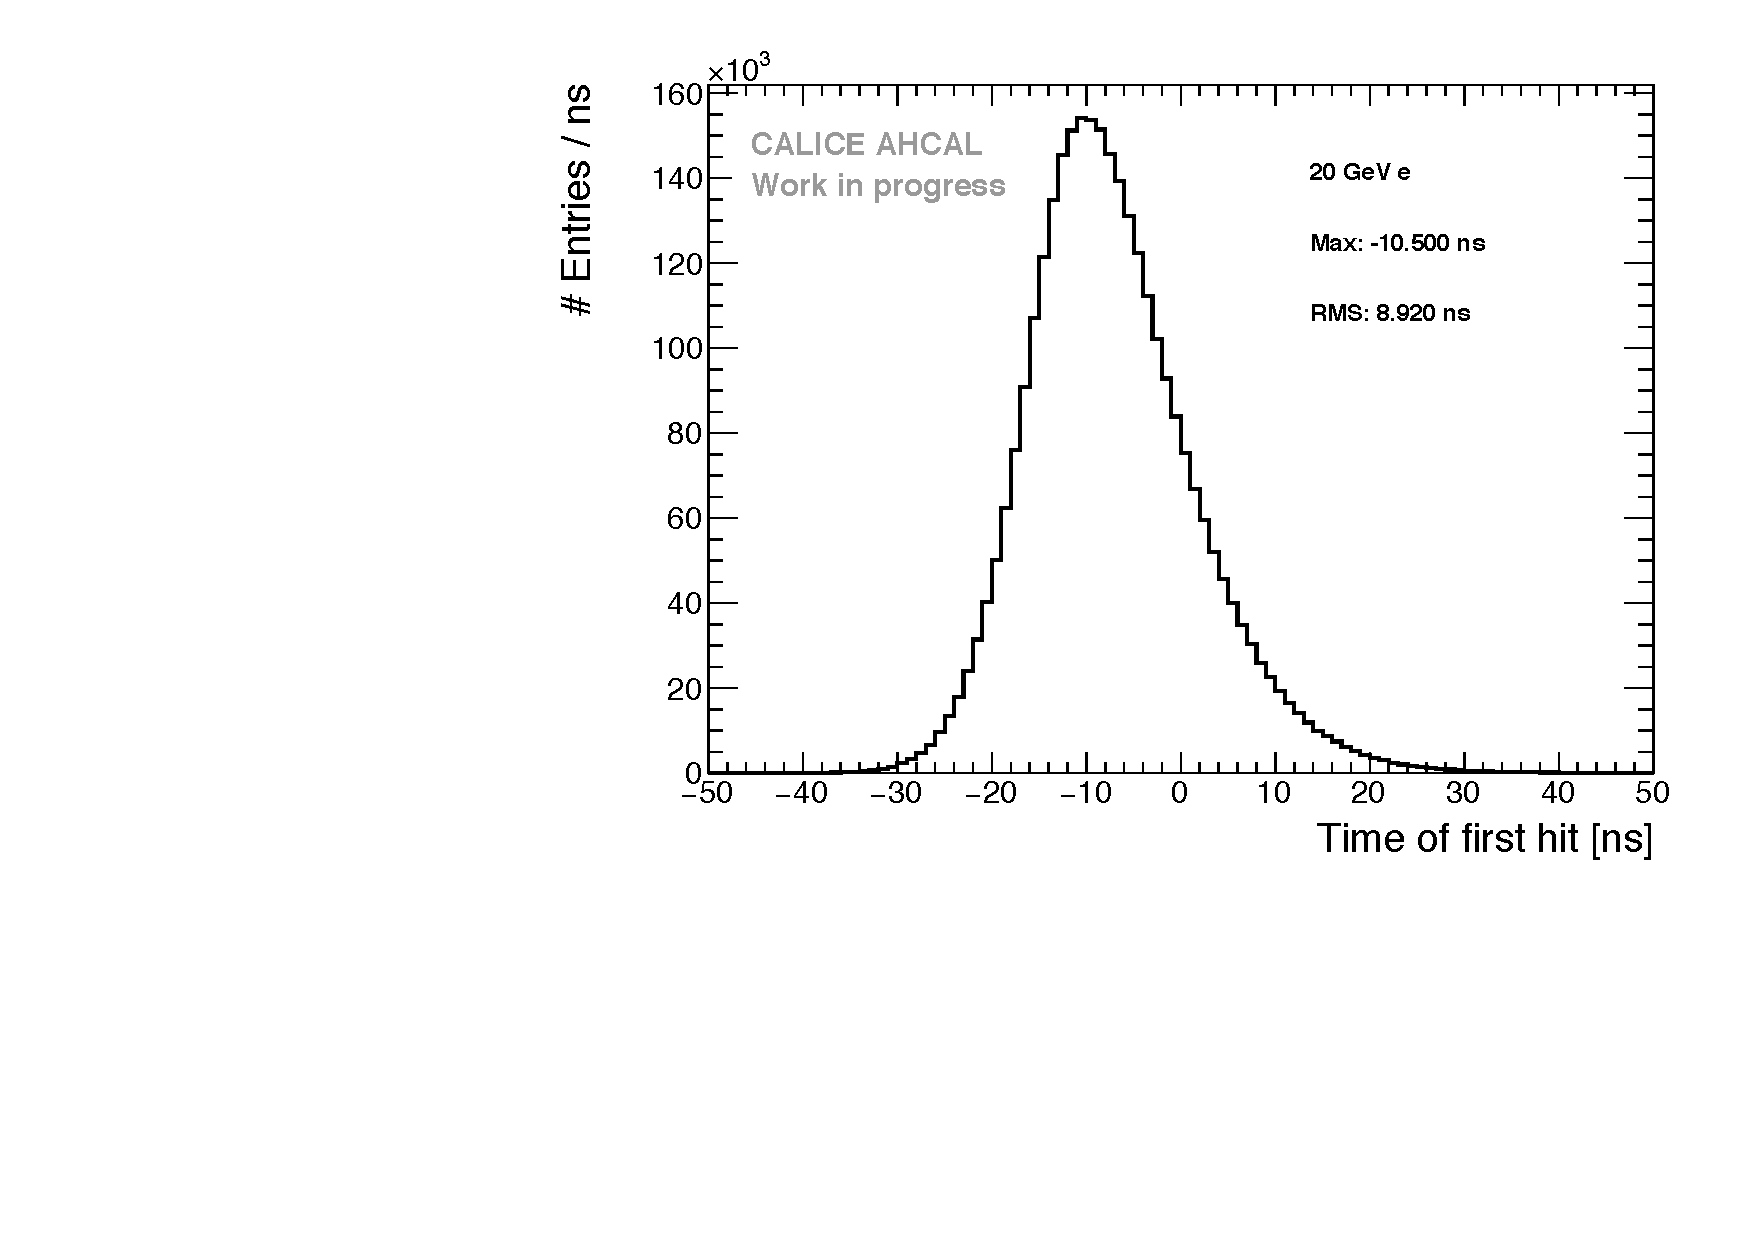
\includegraphics[width=0.6\textwidth]{fig/Electrons/Timing_AllLayers_AfterMuons.pdf}
\caption{Time of the first hit distribution for 20 GeV electrons, Max = 10.05 ns, RMS = 8.92 ns.}
\label{fig:Timing_electrons}
\vspace{-6ex}
\end{center}
\end{figure}

\subsection{Influence of the number of triggered channels}
\label{subsec:ped_shift}

Pedestal shift for energy measurement is not a new feature of the SPIROC2b chip \cite{OskarMaster}. This electronic effect may be also present for timing measurement. It can be investigated by looking at the time of the first hit as a function of the number of triggered channels over 0.5 MIP. It is shown in figure \ref{fig:nhits_profile}. This can be drastic on the time measurement of the AHCAL, a correction up to 15-20 ns can be necessary to the data for a high number of trigger. The correction parameters are determined by a linear fit to the data.

\begin{figure}[htbp]
	\subfigure[Time of the first hit function of the number of triggered channels in a chip (20 GeV).\label{fig:nhits_profile}] {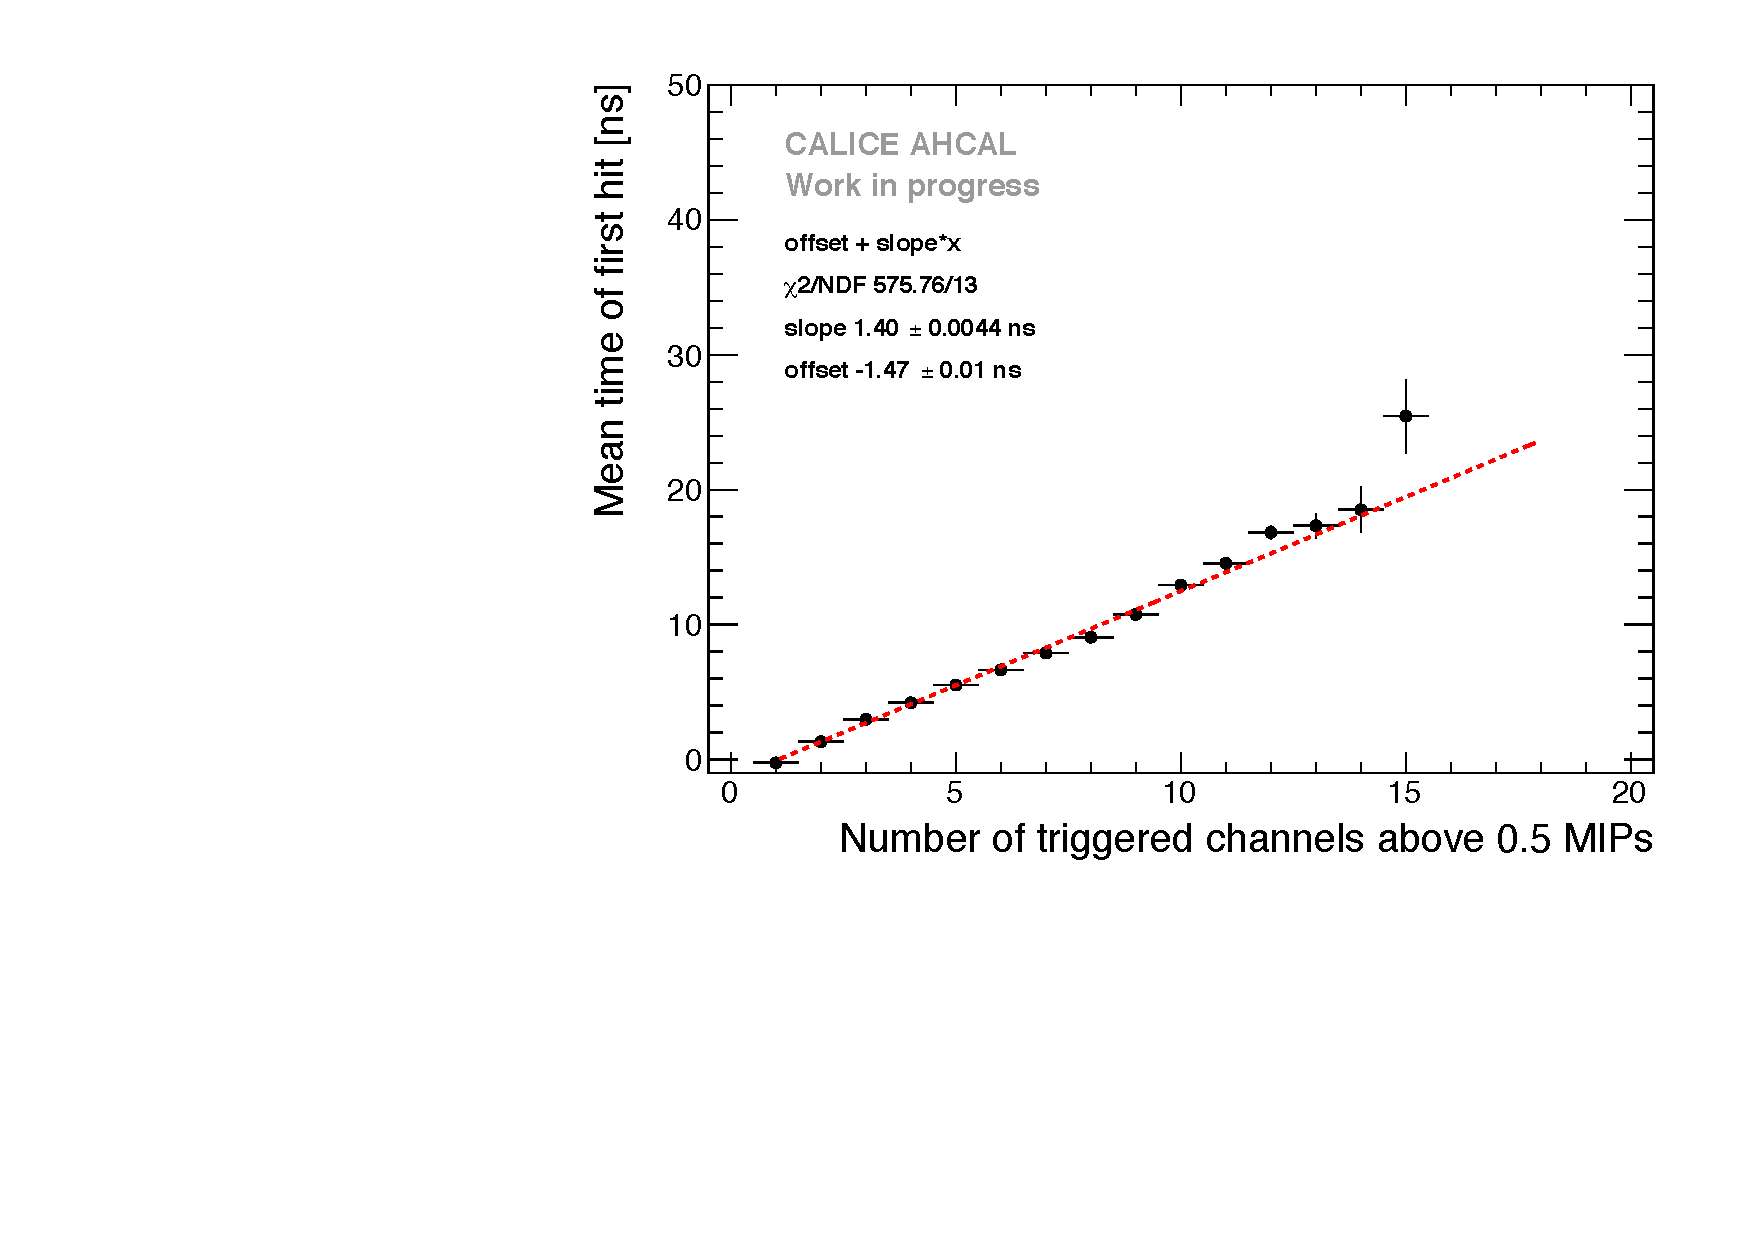
\includegraphics[width=0.5\textwidth]{fig/Electrons/NumberHits_Dependance.pdf}}\hfill
	\subfigure[RMS of the time of first hit function of the number of triggered channels (20 GeV).\label{fig:RMS_nHits}] {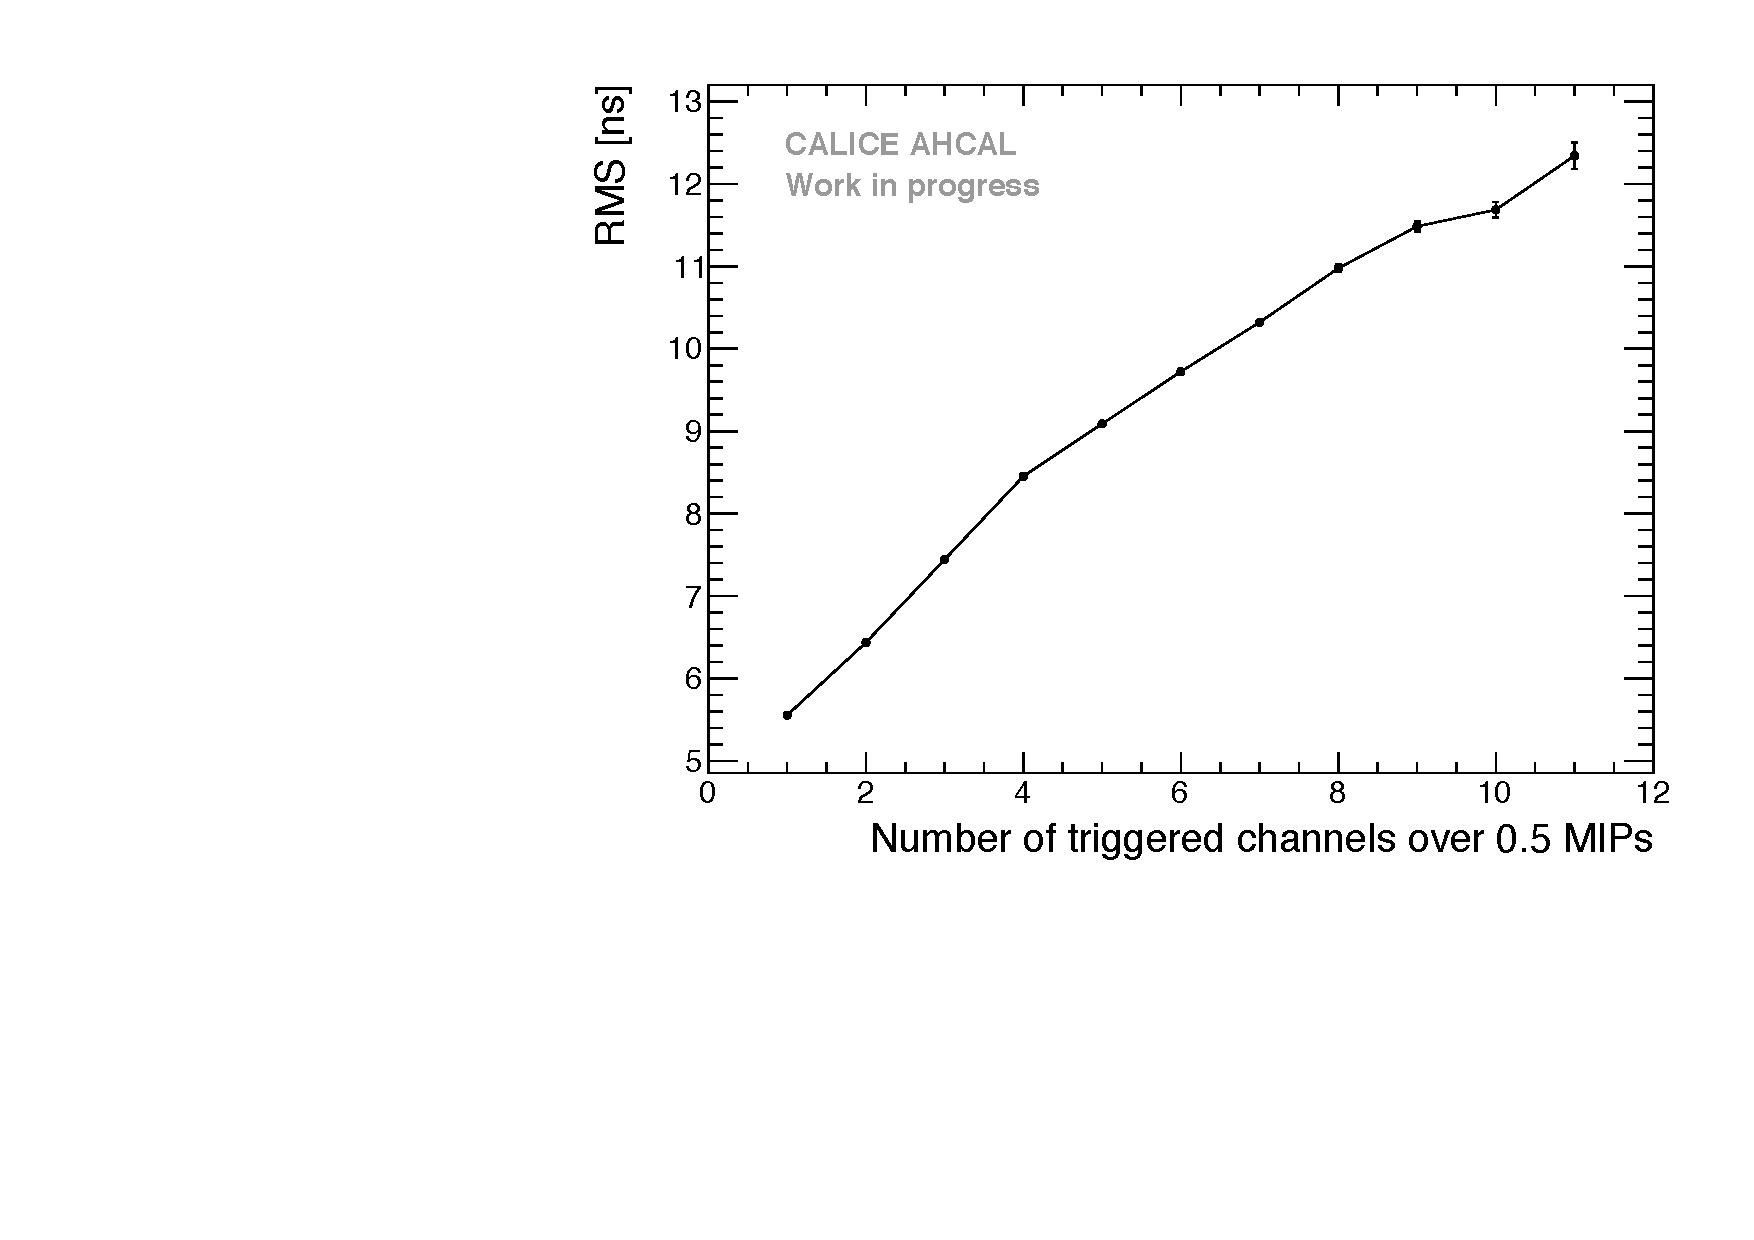
\includegraphics[width=0.5\textwidth]{fig/Electrons/ParametrisationPedestalShift_20GeV.pdf}}
	\caption[]{\textbf{a}: The fit region is between 1 and 15 hits. A linear dependence is clearly visible. \textbf{b}: The RMS of the time distribution can increase up to 12 ns for a high number of triggered channels.}
\end{figure}

\subsection{Time of the first hit for electrons}
\label{subsec:Electron_Final}

\begin{figure}[htbp]
	\subfigure[Time of the first hit distribution for 20 GeV electrons after correction.\label{fig:timing_electrons_corr}] {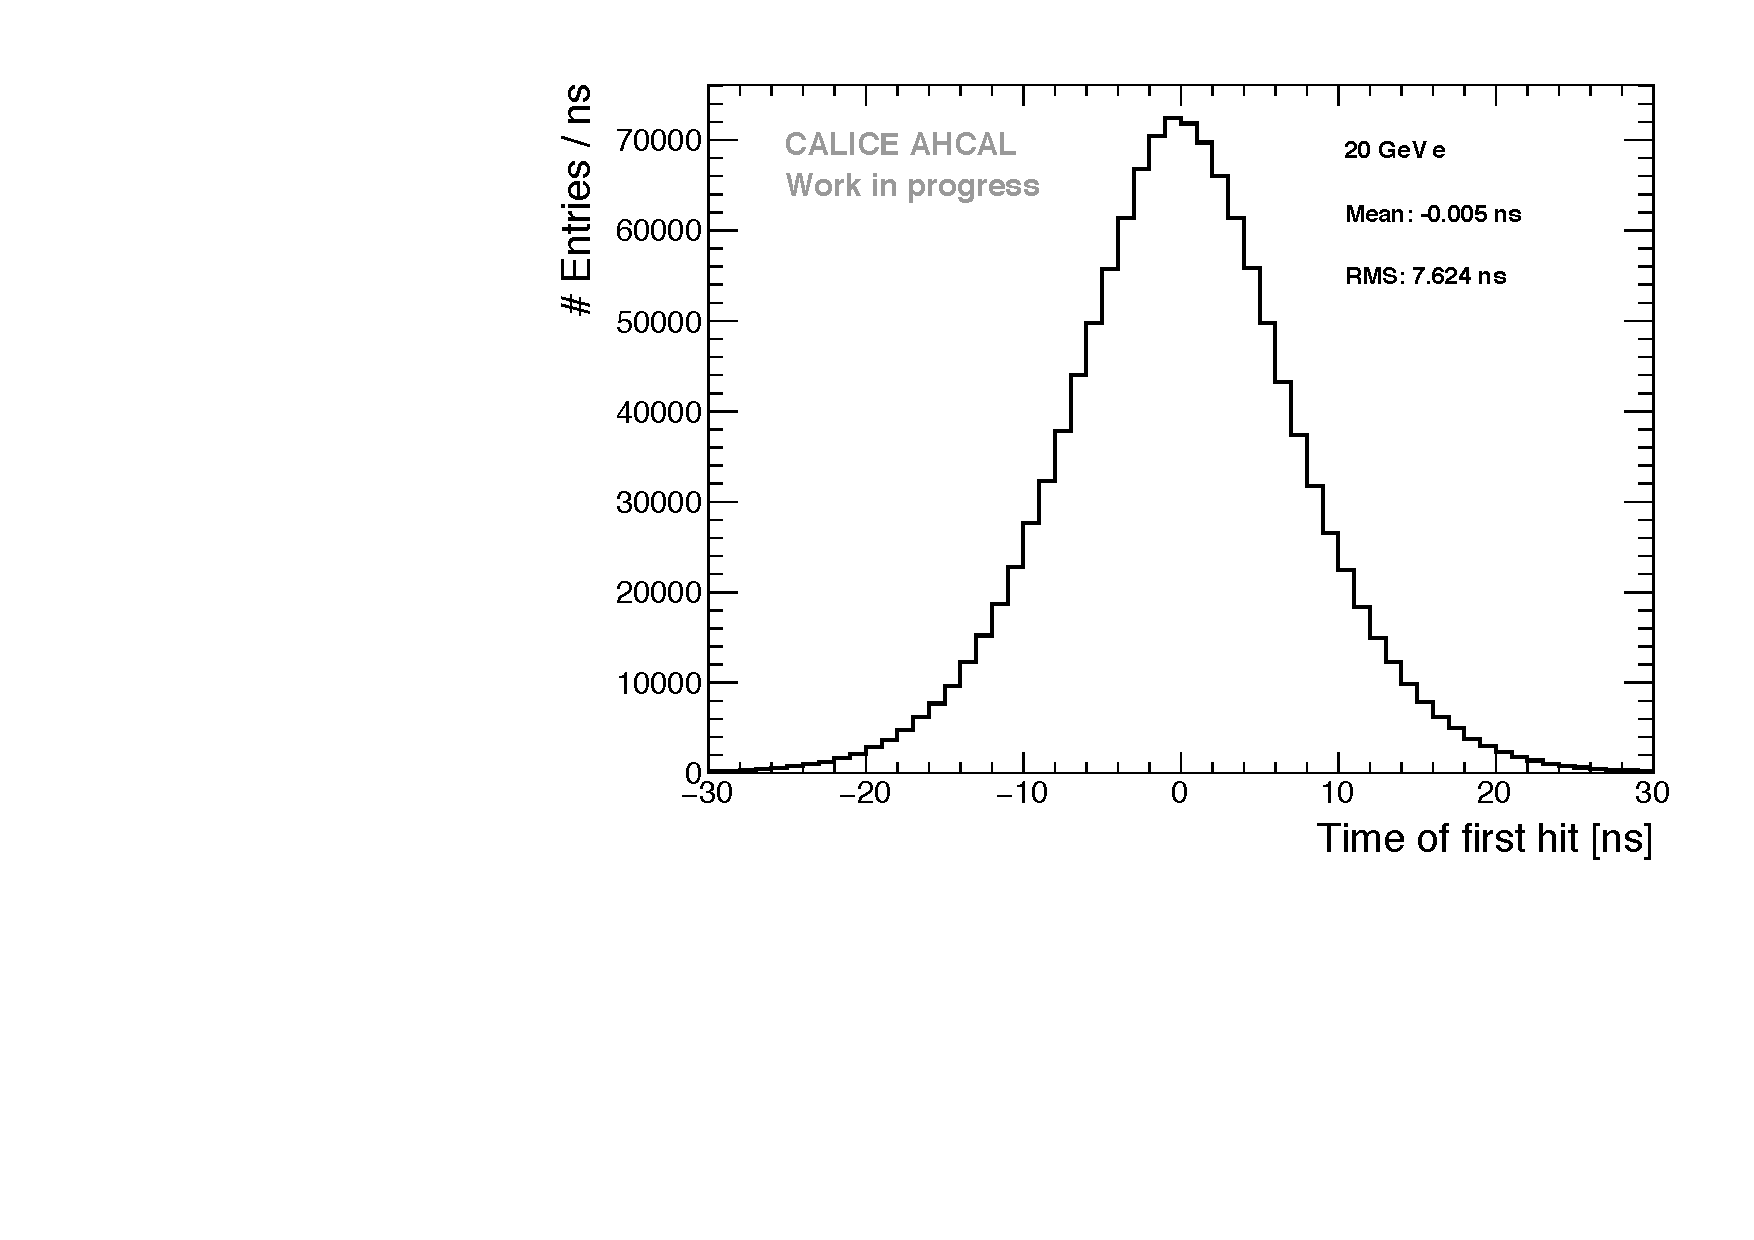
\includegraphics[width=0.5\textwidth]{fig/Electrons/Timing_AllLayers_20GeV.pdf}}\hfill
	\subfigure[Comparison with the muon time of first hit distribution.\label{fig:timing_electron_muon_comp}] {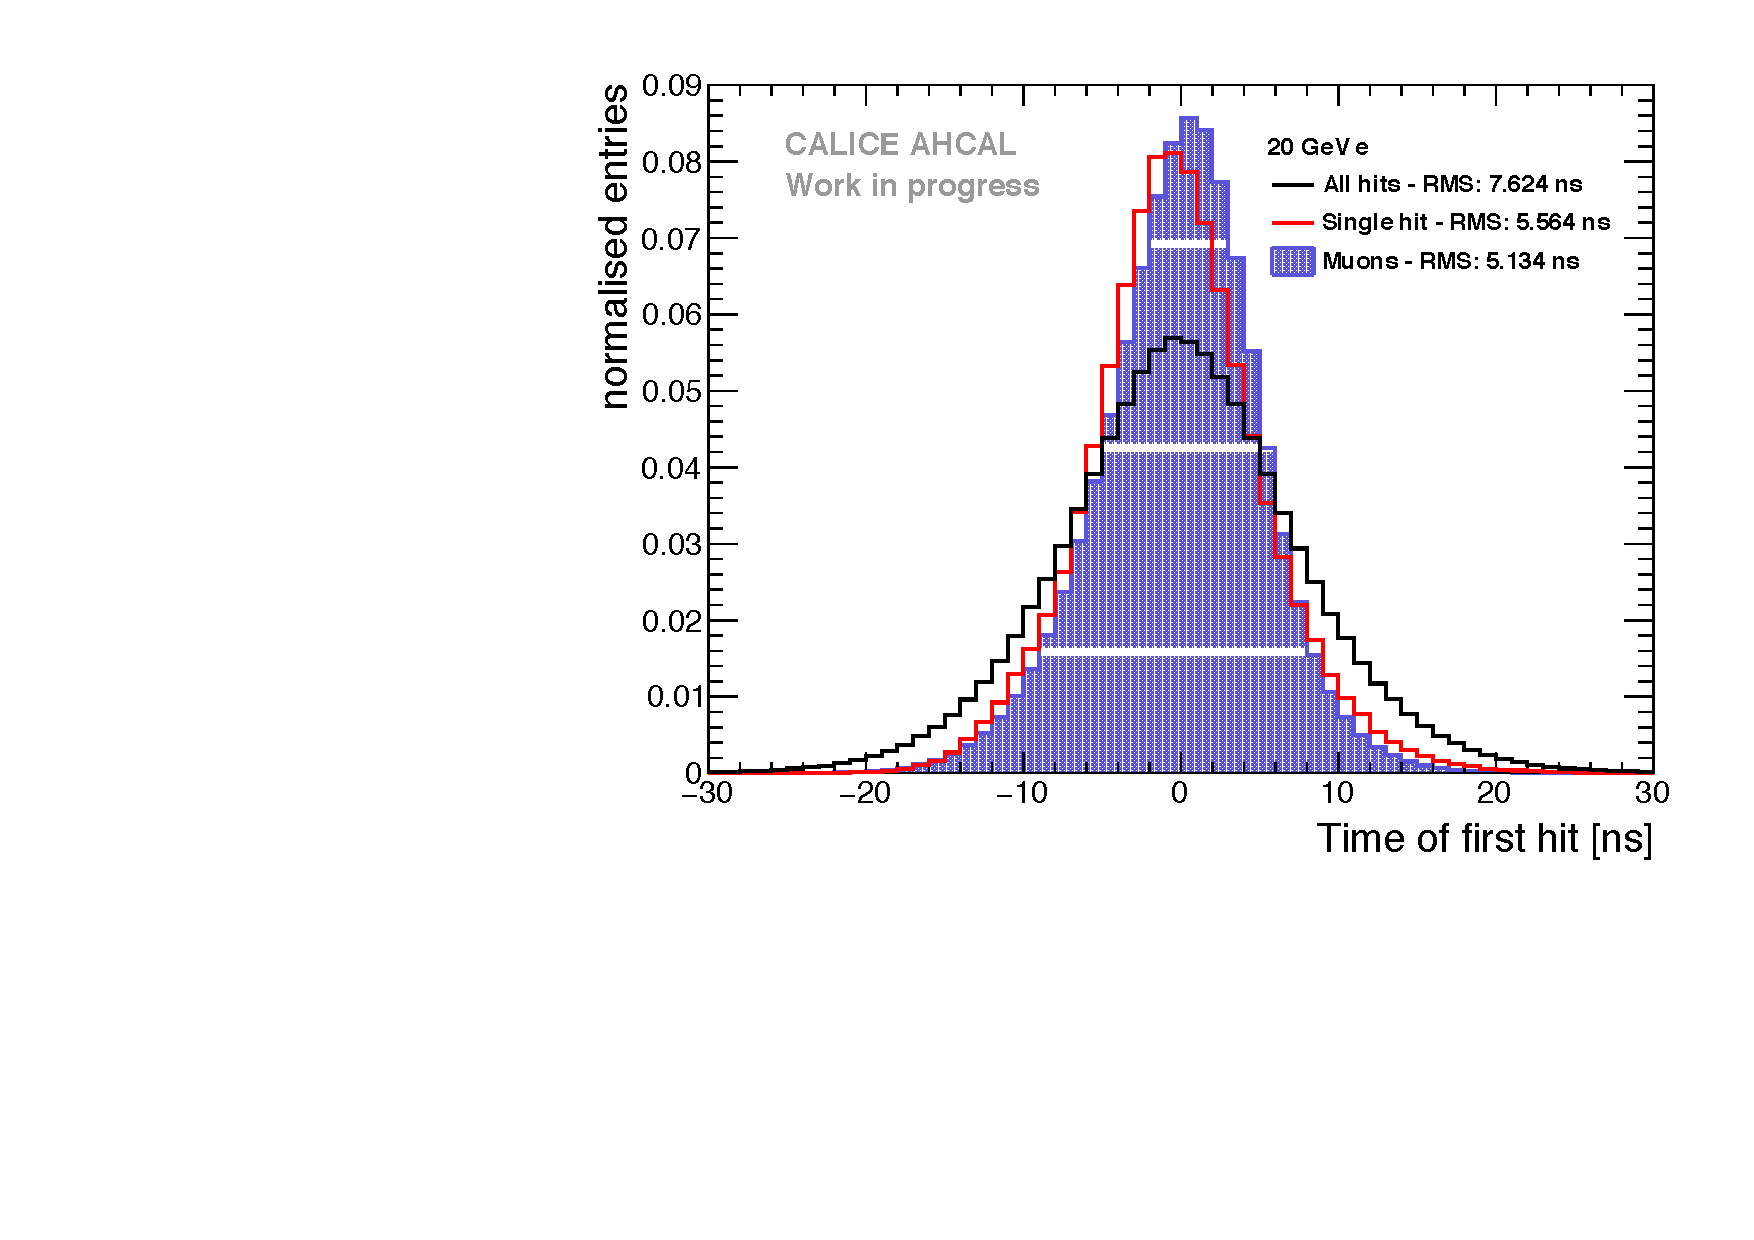
\includegraphics[width=0.5\textwidth]{fig/Electrons/ComparisonAll_ElectronsSingleHit.pdf}}
	\caption[]{\textbf{a}: Time of the first hit distribution for 20 GeV electrons after number of triggered channel correction, $\mu$ = -0.005 ns, RMS = 7.62 ns. \textbf{b}: Comparison of the electron data sample, the time distribution is very similar to the muon one if only events with single hits in a chip are taken.}
\end{figure}

The distribution of the time of the first for 20 GeV is shown in figure \ref{fig:timing_electrons_corr} after correction. As seen the correction improves the RMS of the distribution ($\sim$14.6\%) as well as the distribution appears more gaussian-like. However, there is still a discrepancy ($\sim$32.6\%) with the time resolution obtained for muons (5 ns). This is due to the fact that not only the mean time shifts but that the RMS also increases as a function of number of hits as seen in figure \ref{fig:RMS_nHits}. In order for the simulation to match the data, the increase of the width of the time distribution has to be parametrised from the data. More details can be read in the appendix \ref{appendix:ped_shift}. A comparison with the muon data has been done in order to cross-check the calibration as seen in figure \ref{fig:timing_electron_muon_comp}. If only single hits in a chip are taken, the time resolution obtained is very similar to the time resolution observed in muons ($\sim$7.7\% difference).\\
The cause of observed effect is most likely due to an element in the chip (a delay box) that get unstable with the number of triggered channels and that is responsible for the hold of the TDC value in the chip. The hold is delayed thus sampling a higher TDC value than the one expected. All electron runs have been checked to validate the correction and calibration procedure. The figure \ref{fig:all_electron_energies} shows the comparison from 10 GeV to 50 GeV. The distributions are in agreement within a 10-15\% range for all energies which is within systematical uncertainty as explained in subsection \ref{subsec:det_inhomo}.

\begin{figure}[htbp]
\begin{center}
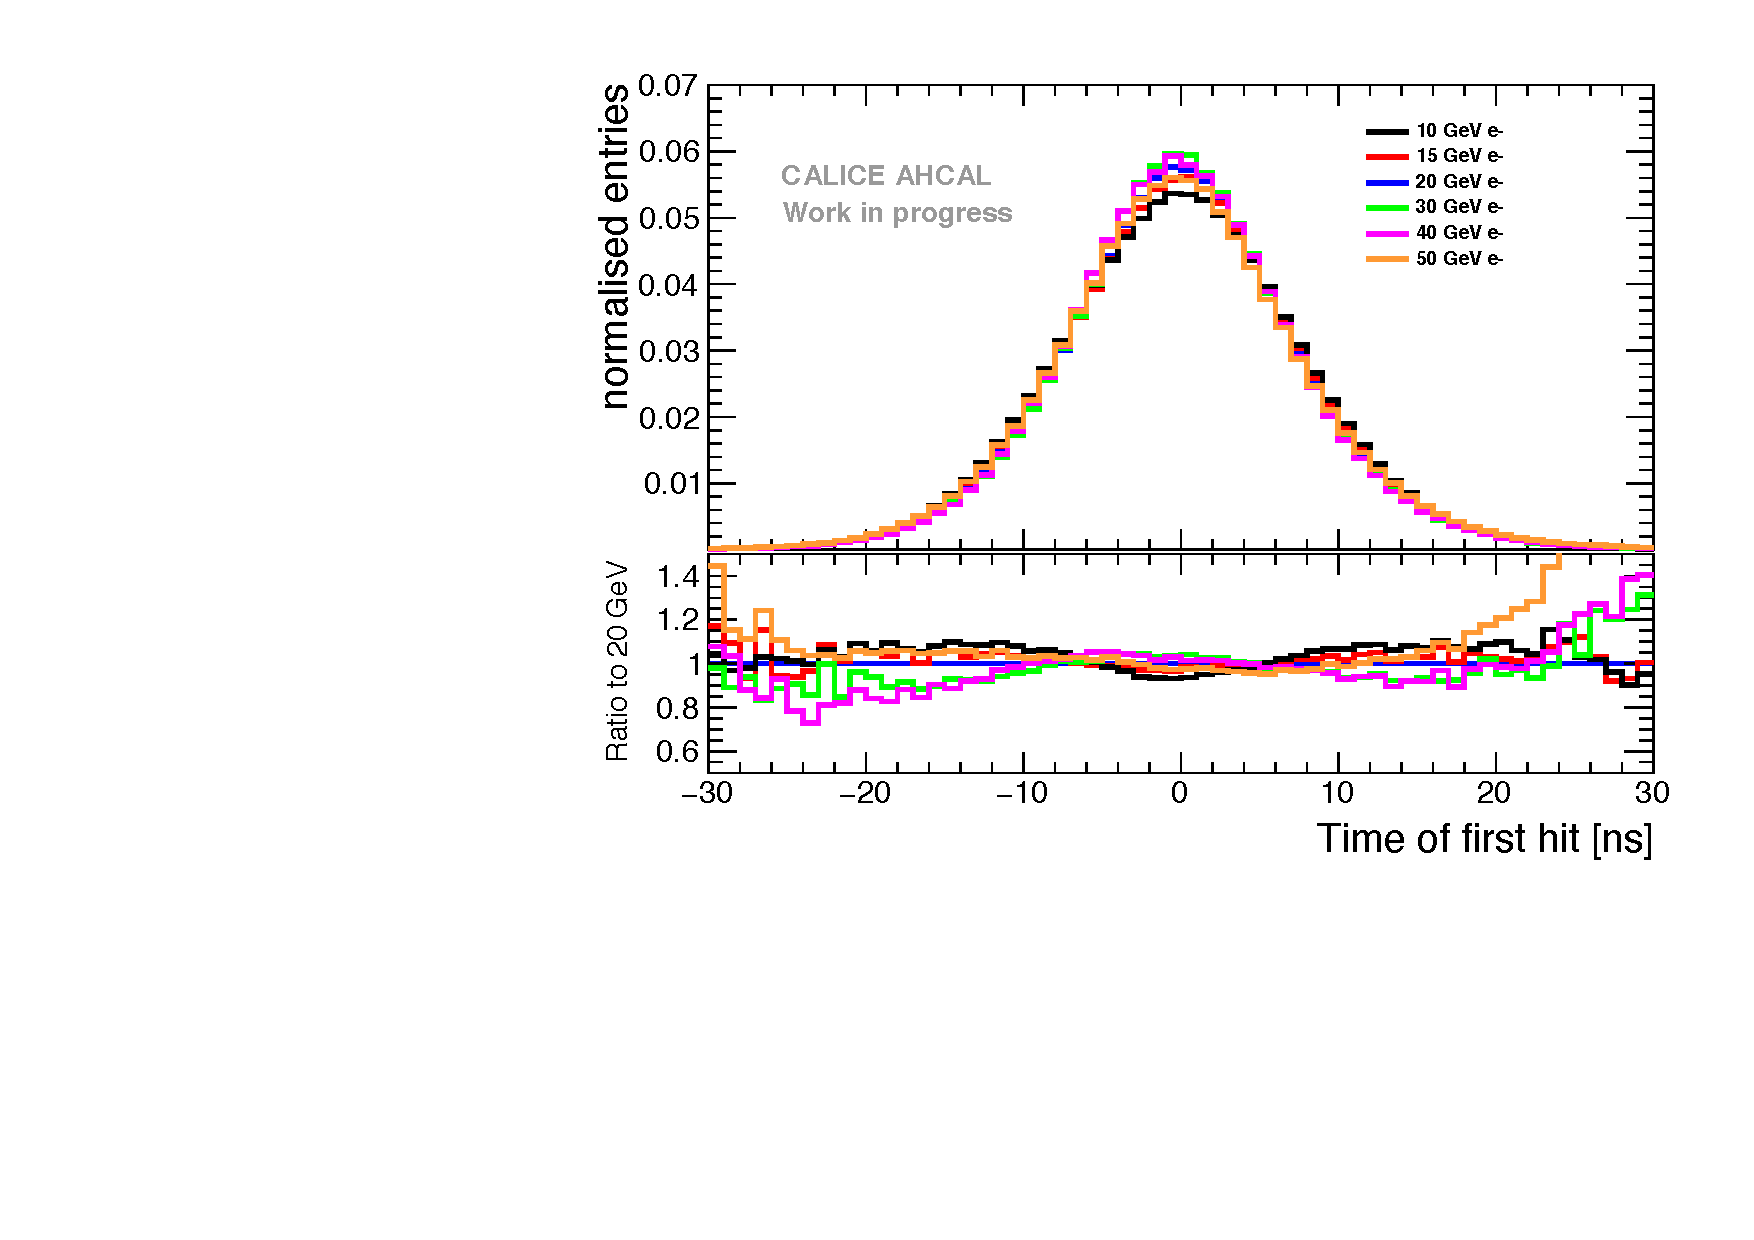
\includegraphics[width=0.6\textwidth]{fig/Electrons/ComparisonDataEnergies.pdf}
\caption{Comparison of the time of first hit distribution for all electron energies.}
\label{fig:all_electron_energies}
\end{center}
\end{figure}

\subsection{Influence of the detector inhomogeneity}
\label{subsec:det_inhomo}

A study has been performed to estimate the influence of the detector inhomogeneity on timing independent of the beam profile. For this, only events in which the centre of gravity in x and y are within the 4 centre tiles of the detector are selected. This has been checked for 10 and 50 GeV electron beam energy. The difference between the distribution can help to estimate the systematic uncertainty due to the inhomogeneity of the detector.
\begin{figure}[htbp]
	\subfigure[Time of the first hit distribution at 10 GeV.\label{fig:timing_inhomo_10GeV}] {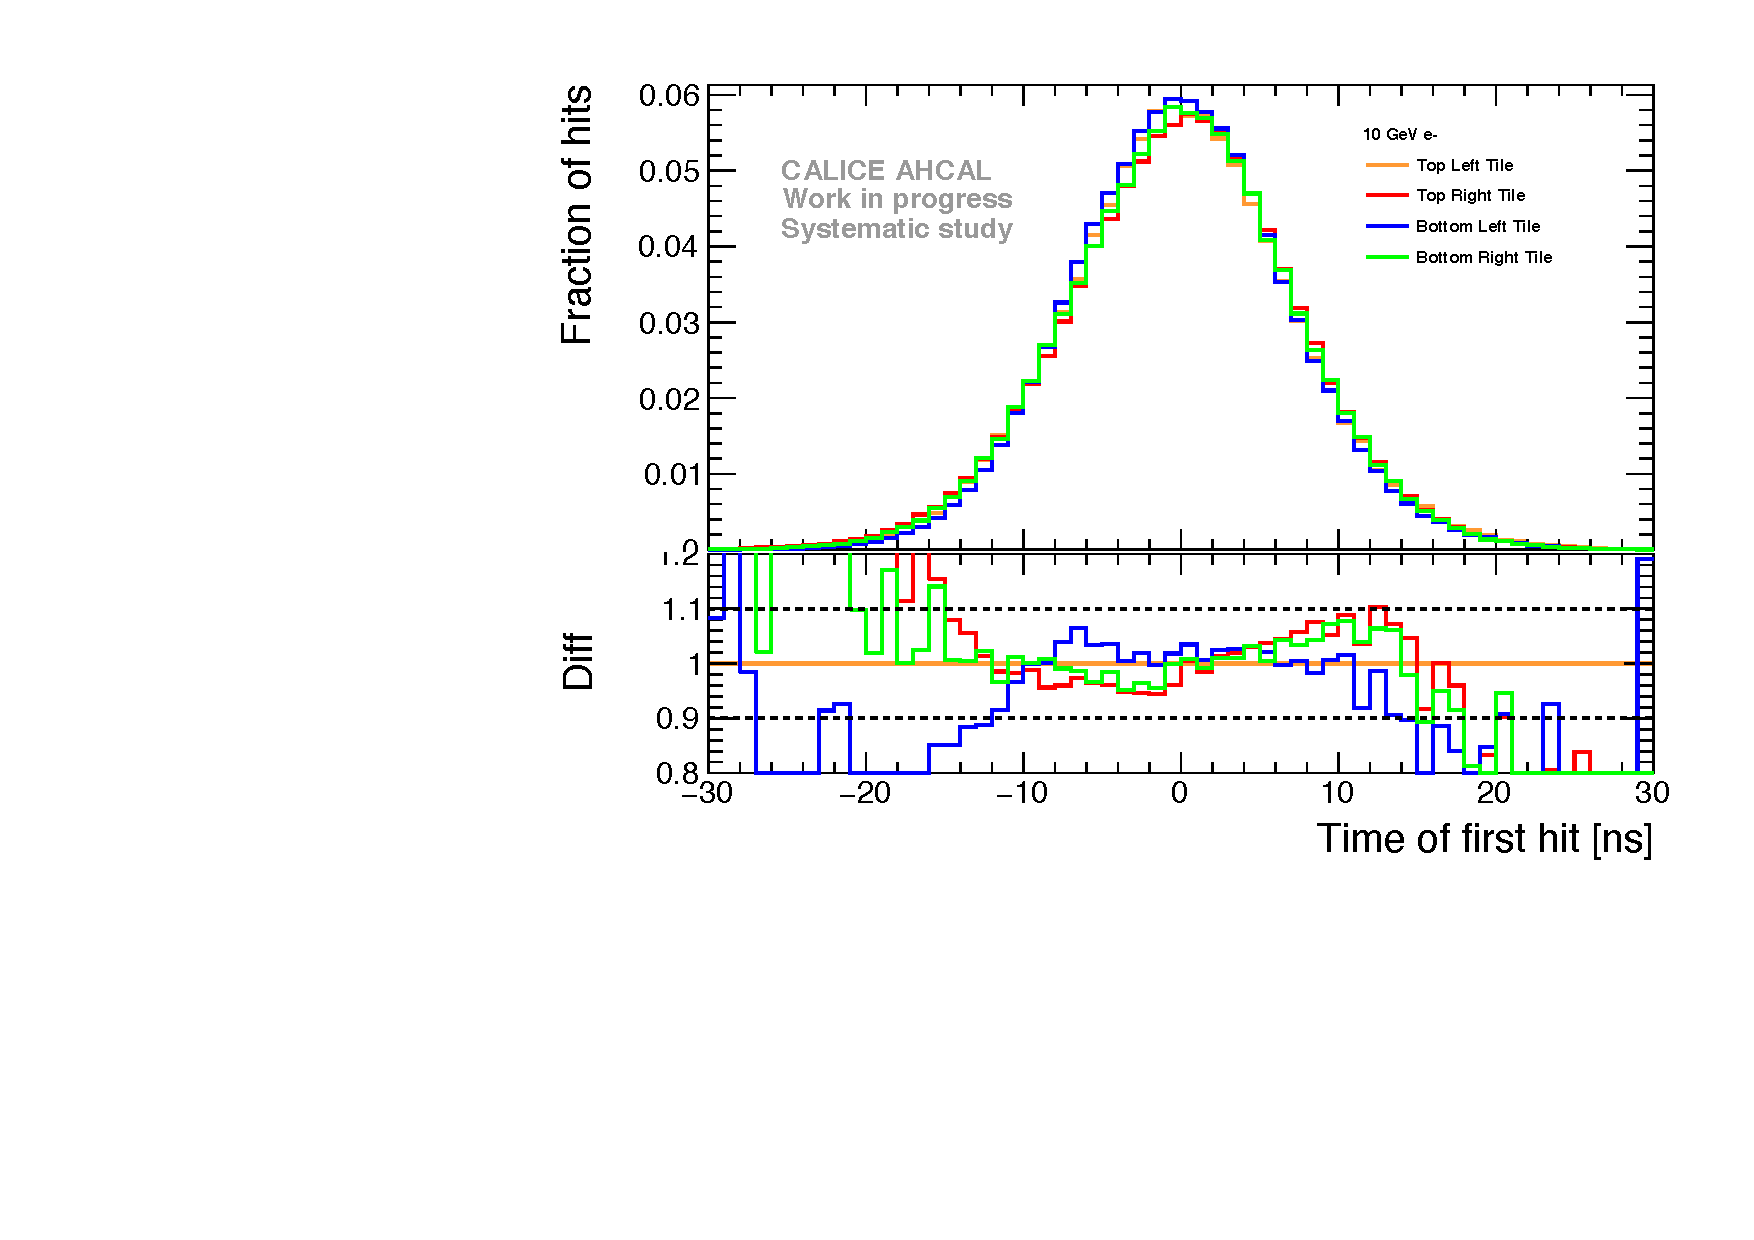
\includegraphics[width=0.5\textwidth]{fig/Electrons/Systematic_Inhomogeneity_10GeV.pdf}}\hfill
	\subfigure[Time of the first hit distribution at 50 GeV.\label{fig:timing_inhomo_50GeV}] {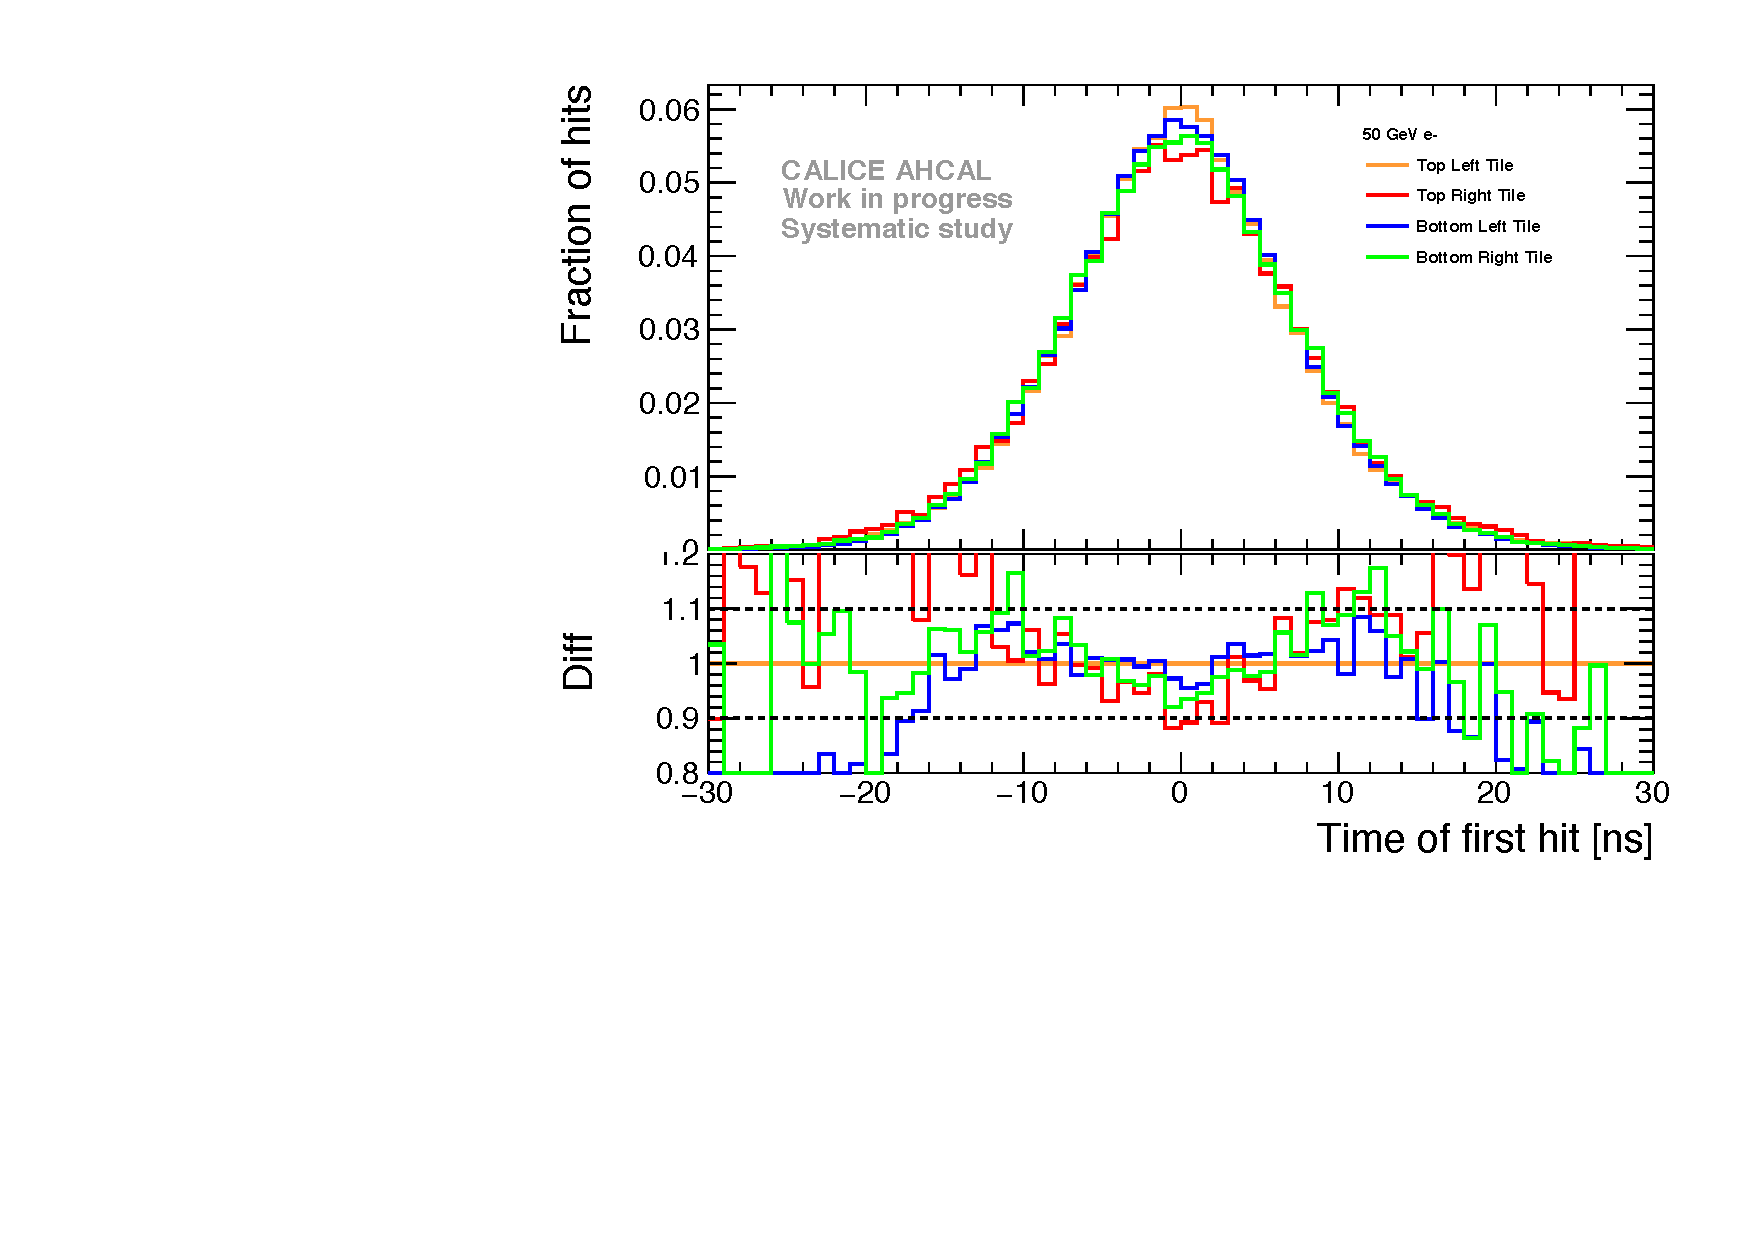
\includegraphics[width=0.5\textwidth]{fig/Electrons/Systematic_Inhomogeneity_50GeV.pdf}}
	\caption[]{\textbf{a}: Time of the first hit distribution for all 4 tiles at 10 GeV. All distribution are within 10-15\% in the core. \textbf{b}: Time of the first hit distribution for all 4 tiles at 50 GeV. All distribution are within 10-15\% in the core.}
\end{figure}
The figures \ref{fig:timing_inhomo_10GeV} and \ref{fig:timing_inhomo_50GeV} show the time distribution for each tiles at 10 and 50 GeV respectively. The ratio shown is compared to the top left centre tile. One can see that for both energies, the distributions are within a 10-15\% agreement. Therefore a conservative systematic uncertainty of 15\% is assigned to electron and pion data in the following.

\section{Validation of the Calibration}

\subsection{Muons}

The next step is to compare data with simulation and cross-check the simulation with electrons. The timing resolution is extracted from muon data runs by fitting a double Gaussian in the range [-50 ns, 50 ns] and is used to smear the timing of simulated hits. The table \ref{table:time_res_sim} sums up the parameters used. The comparison for muons is shown in figure \ref{fig:sim_data_muon}. The comparison shows that in the full range, the difference between data and simulation is around 10-20\% maximum. This may be because of the asymmetry present in data that might be not well reproduced in Monte-Carlo. In general, the simulation is in a good agreement with data.

\begin{table}[htbp]
\centering
  \begin{tabular}{@{} cccc @{}}
    \hline
    $\mu_{1}$ [ns] & $\sigma_{1}$ [ns] & $\mu_{2}$ [ns] & $\sigma_{2}$ [ns] \\
    \hline
    -0.699095 & 5.8589 & 0.945278 & 3.40119 \\
    \hline
  \end{tabular}
  \caption[Timing resolution extracted with a double Gaussian fit from muon data used for simulation.]{Timing resolution extracted with a double Gaussian fit from muon data used for simulation.\footnotemark[1]}
  \label{table:time_res_sim}
\end{table}
\footnotetext{A table of rejected chips is available in appendix \ref{appendix:rejection}.}

\begin{figure}[htbp]
	\centering
	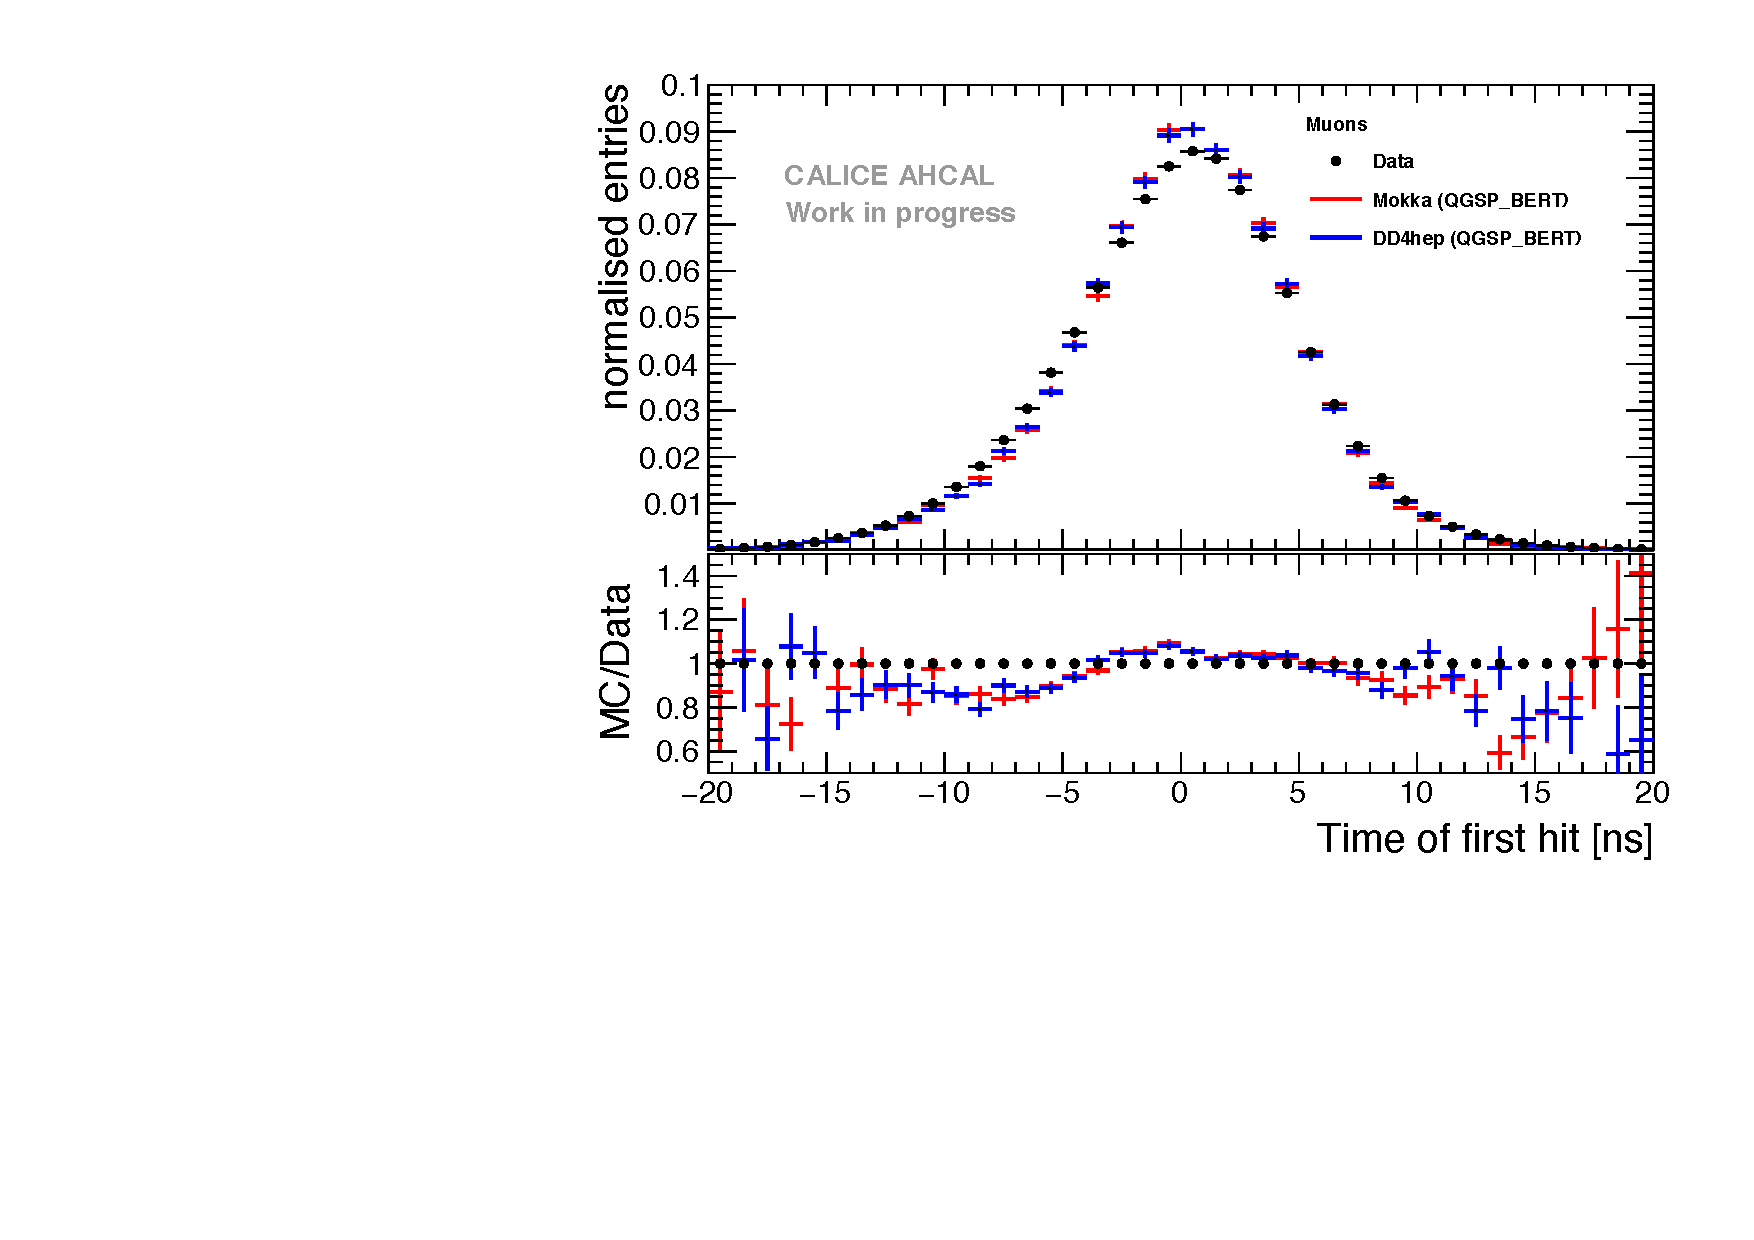
\includegraphics[width=0.6\textwidth]{fig/Muons/Comparison_MokkaDD4hepData_Muons.pdf}
	\caption{Time of first hit for data and simulation between -20 and 20 ns.}
	\label{fig:sim_data_muon}
\end{figure}

\subsection{Electrons}

In the next step, a comparison with electron data is necessary to validate the simulation. In addition to the muon resolution, a parametrisation of the increase of the width of the time distribution function of the number of hits above 0.5 MIPs is added in simulation as described in appendix \ref{appendix:ped_shift}. The figure \ref{fig:sim_data_elec} shows this comparison. The simulation is systematically narrower than data for all energies. This would suggest that simulation has less hits than data which is in agreement with figure \ref{fig:sim_data_elec_nHits}, where generally simulation is 10-20\% lower than data in the region of interest of 6 to 10 hits per chip. The simulation is in better agreement for higher energies (40-50 GeV) than for lower energies (10-15 GeV). This might come from the inhomogeneity of the detector that is not well reproduced in simulation by the global time parametrisation used. This may suggest that the time parametrisation is chip-wise of layer-wise. But due to the limited amount of data, only a global time parametrisation can be applied. For 10 to 20 GeV comparisons, the description of the tails in simulation are quite underestimated. This may be due to the description of the noise in simulation that is not perfectly reproduced. Overall, the simulation and data are in agreement within uncertainties.

\begin{figure}[htbp]
	\subfigure[10 GeV.\label{fig:elec_sim_data_10GeV}] {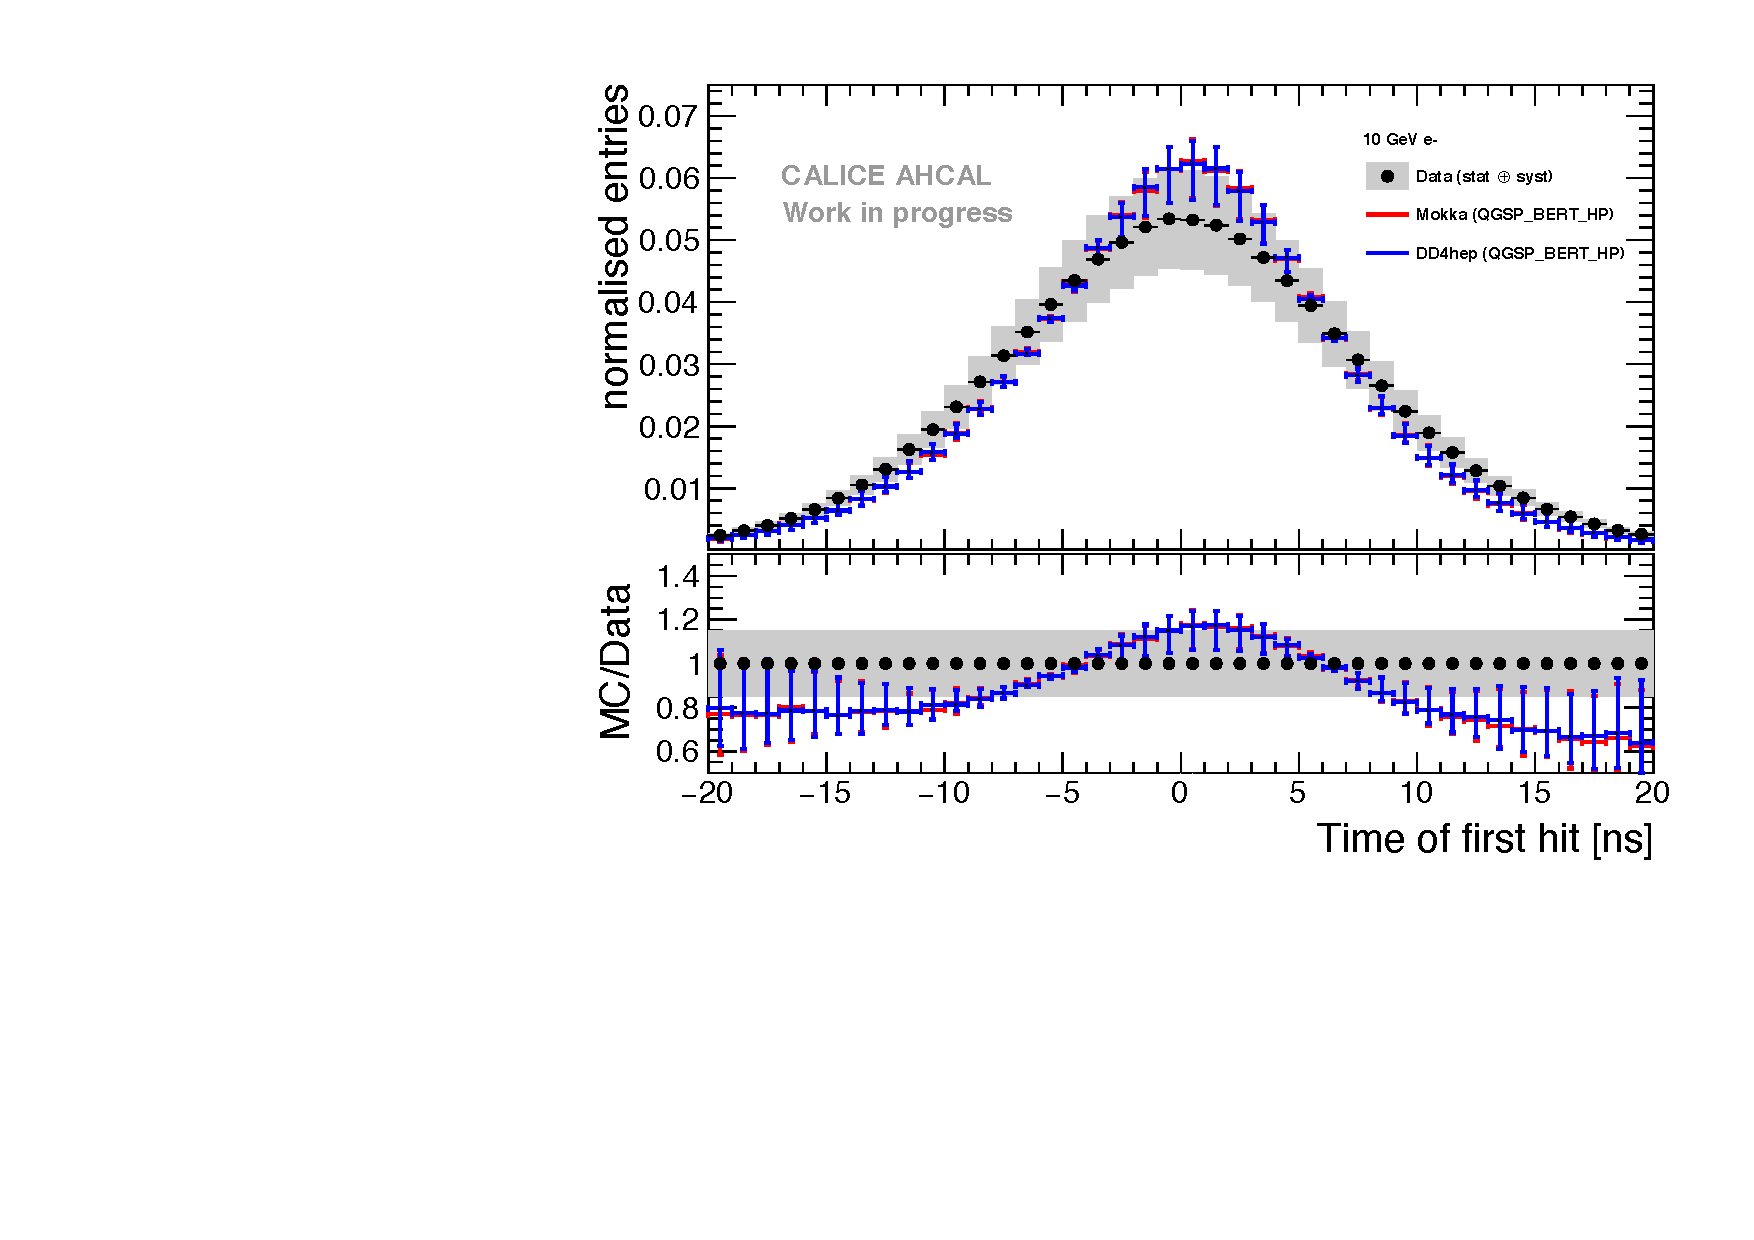
\includegraphics[width=0.5\textwidth]{fig/Electrons/Comparison_SimData_Electrons10GeV.pdf}}\hfill
	\subfigure[15 GeV.\label{fig:elec_sim_data_15GeV}] {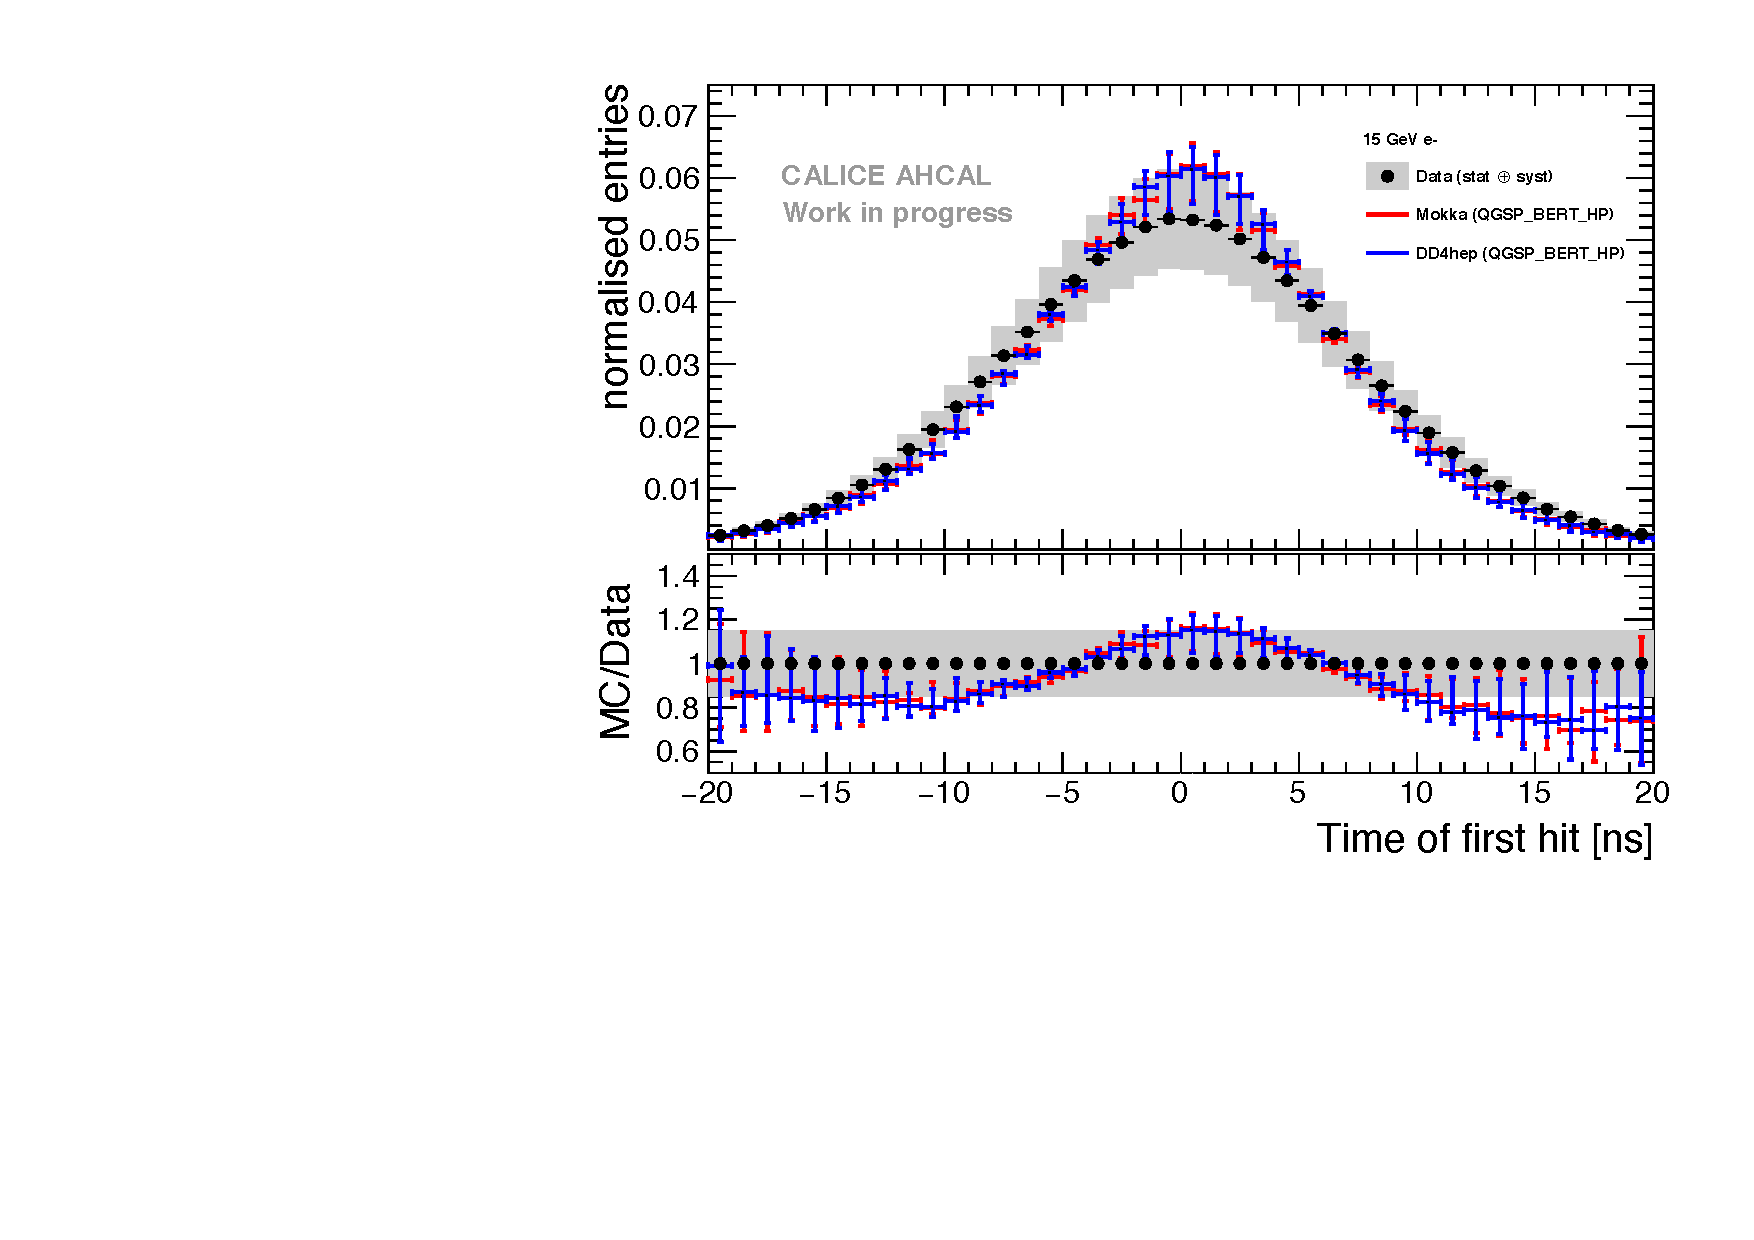
\includegraphics[width=0.5\textwidth]{fig/Electrons/Comparison_SimData_Electrons15GeV.pdf}}\hfill
	\subfigure[20 GeV.\label{fig:elec_sim_data_20GeV}] {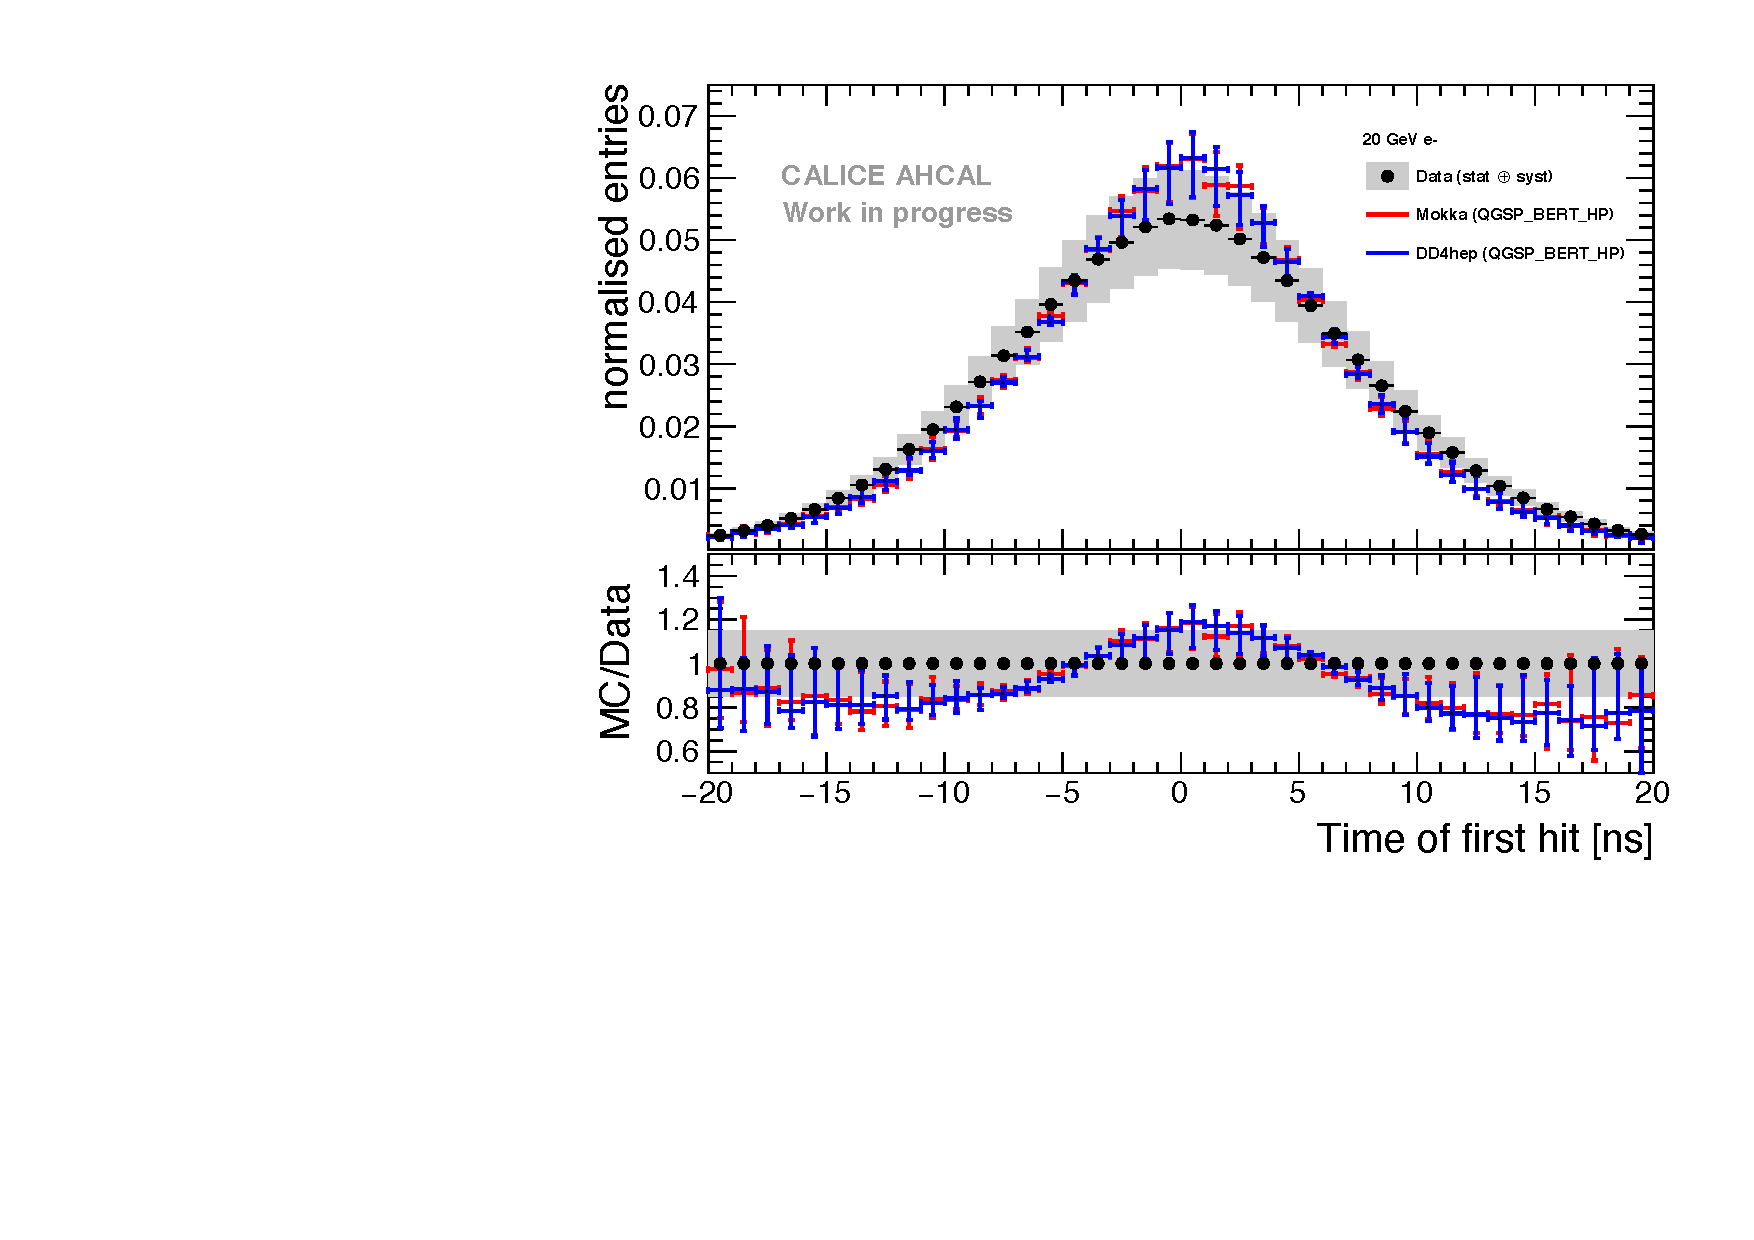
\includegraphics[width=0.5\textwidth]{fig/Electrons/Comparison_SimData_Electrons20GeV.pdf}}\hfill
	\subfigure[30 GeV.\label{fig:elec_sim_data_30GeV}] {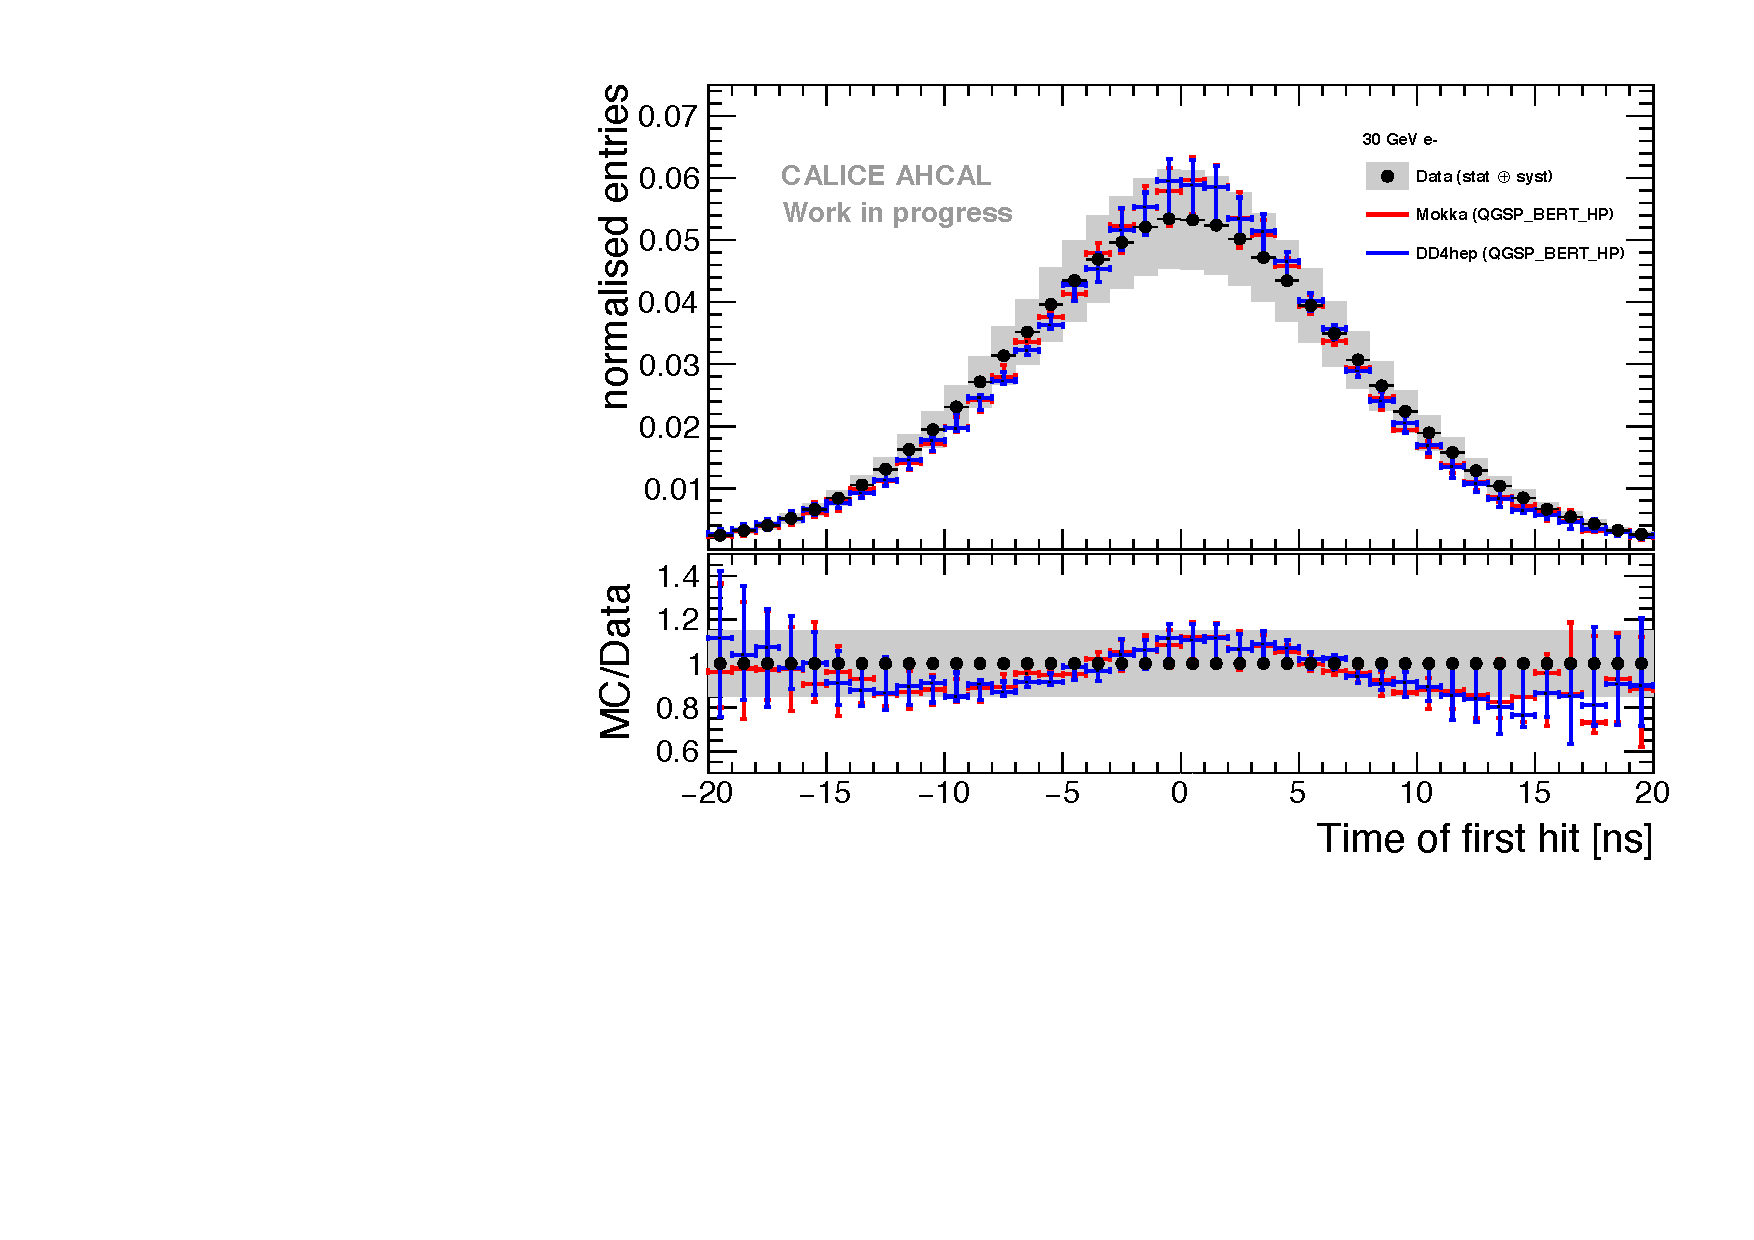
\includegraphics[width=0.5\textwidth]{fig/Electrons/Comparison_SimData_Electrons30GeV.pdf}}\hfill
	\subfigure[40 GeV.\label{fig:elec_sim_data_40GeV}] {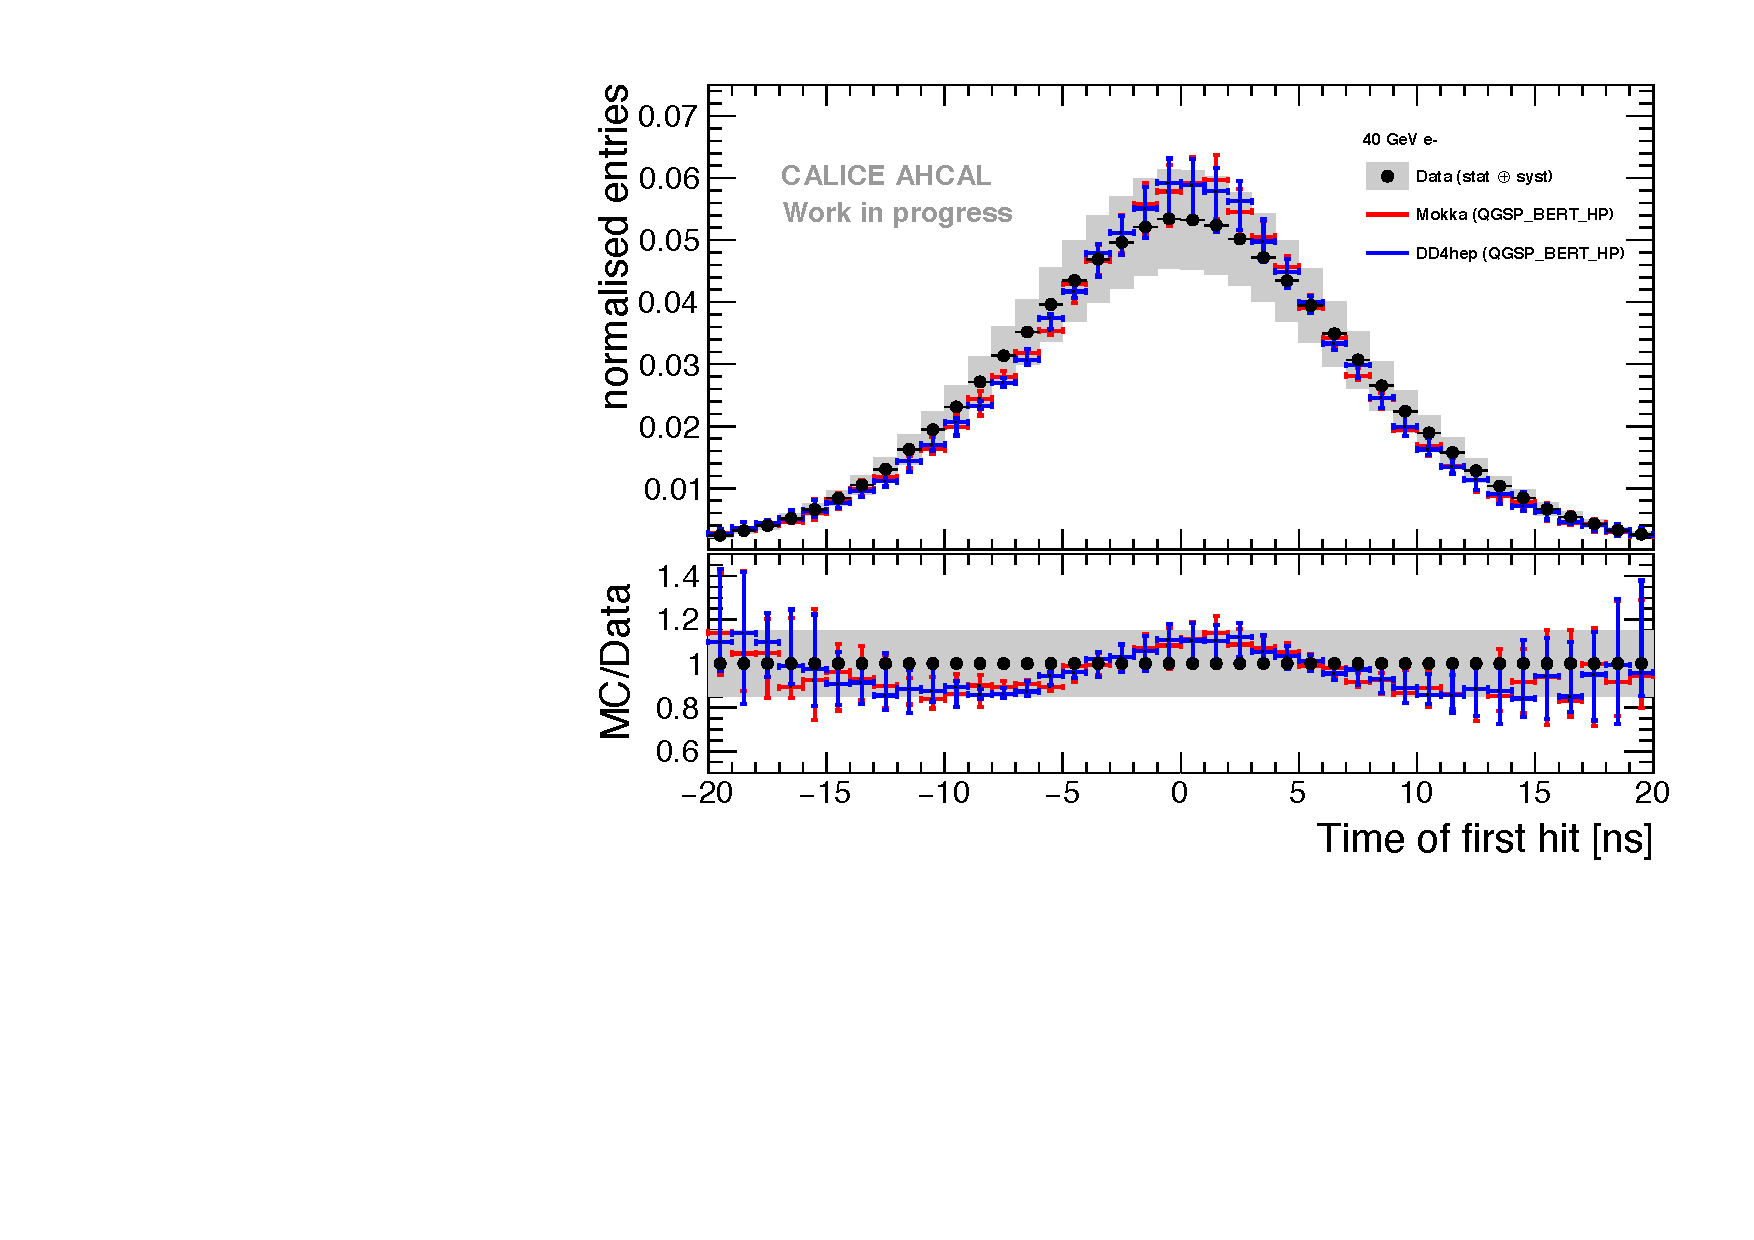
\includegraphics[width=0.5\textwidth]{fig/Electrons/Comparison_SimData_Electrons40GeV.pdf}}\hfill
	\subfigure[50 GeV.\label{fig:elec_sim_data_50GeV}] {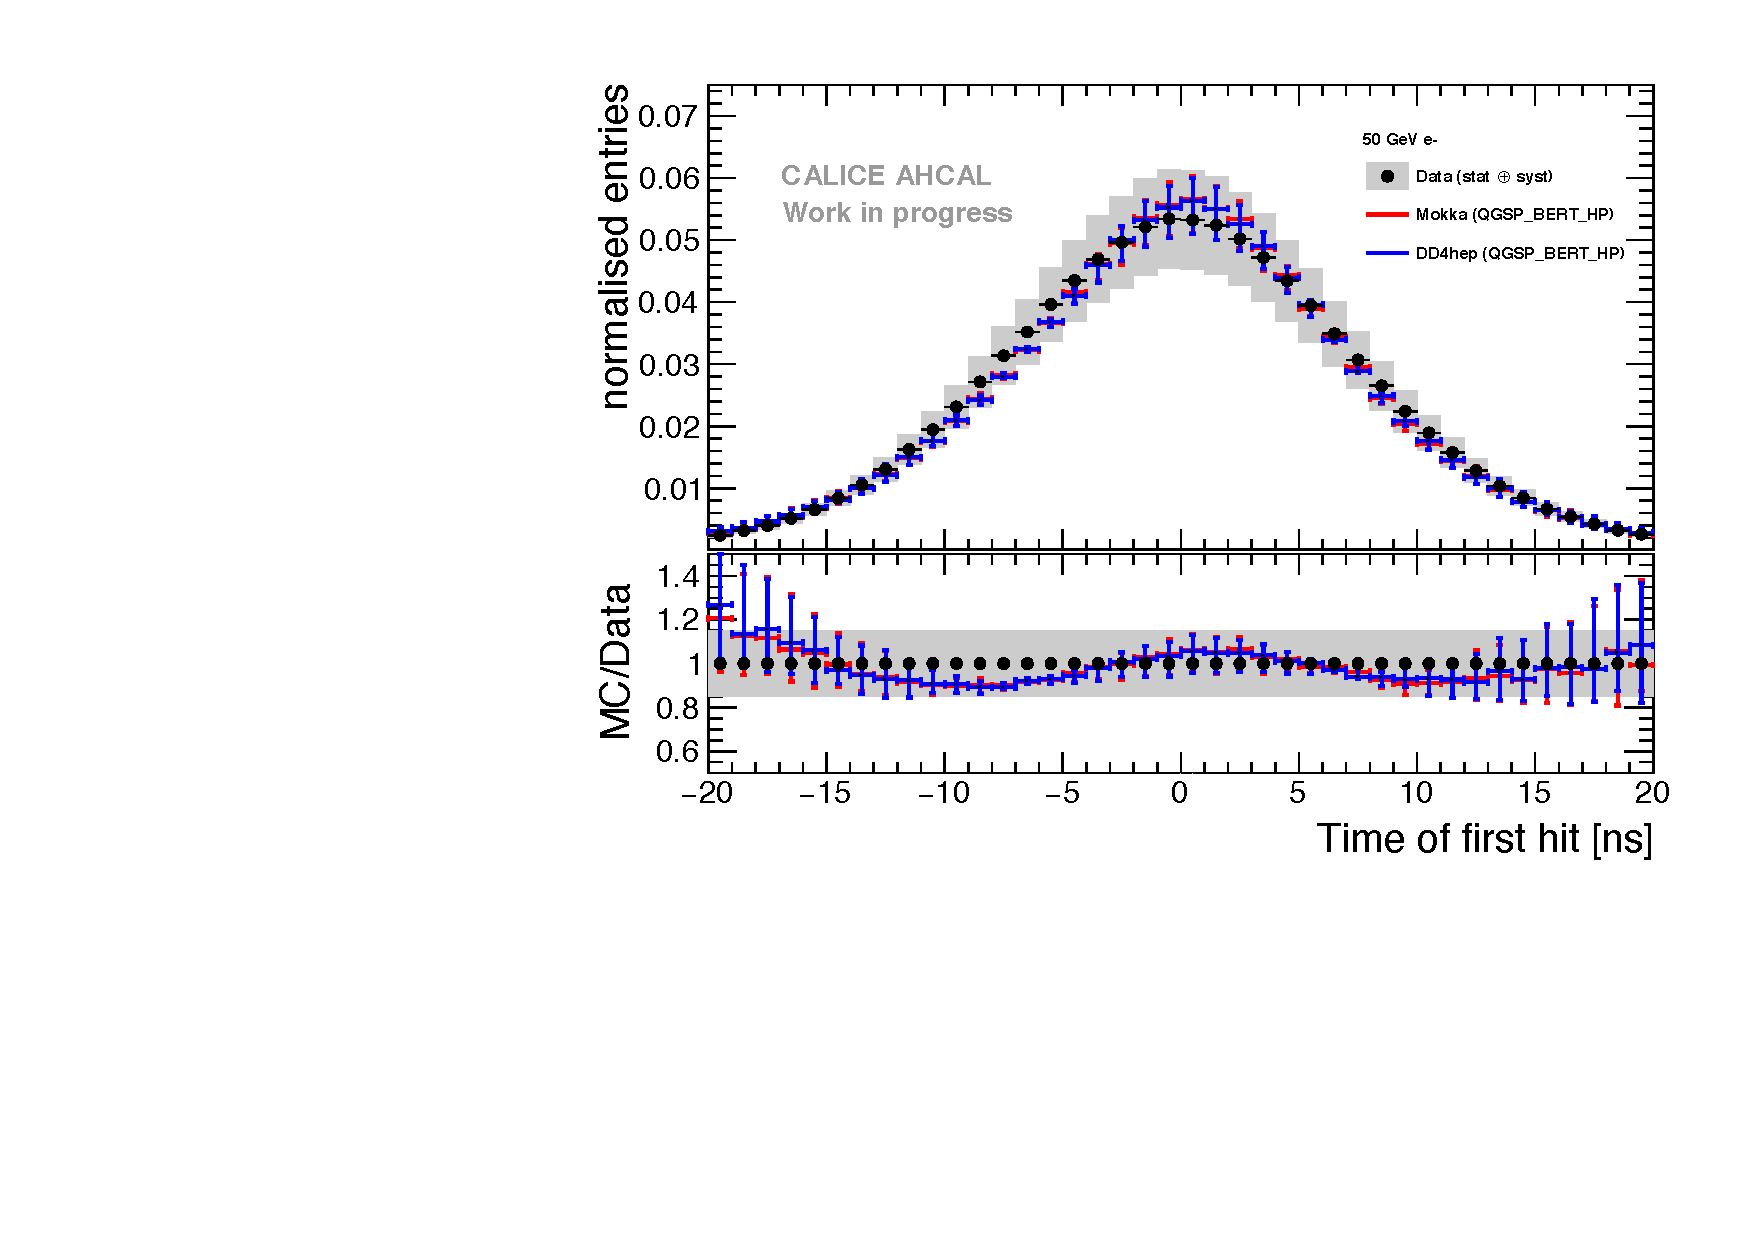
\includegraphics[width=0.5\textwidth]{fig/Electrons/Comparison_SimData_Electrons50GeV.pdf}}\hfill
	\caption[]{Comparison between electron data and MC for all energies of the time of first hit. The grey area represents the statistical and systematical error of the data. Error bars in simulation are obtained by varying the cross-talk parameter and with the error envelope from the number of hits parameterisation.}
	\label{fig:sim_data_elec}
\end{figure}

\begin{figure}[htbp]
	\subfigure[10 GeV.\label{fig:elec_sim_data_nHits_10GeV}] {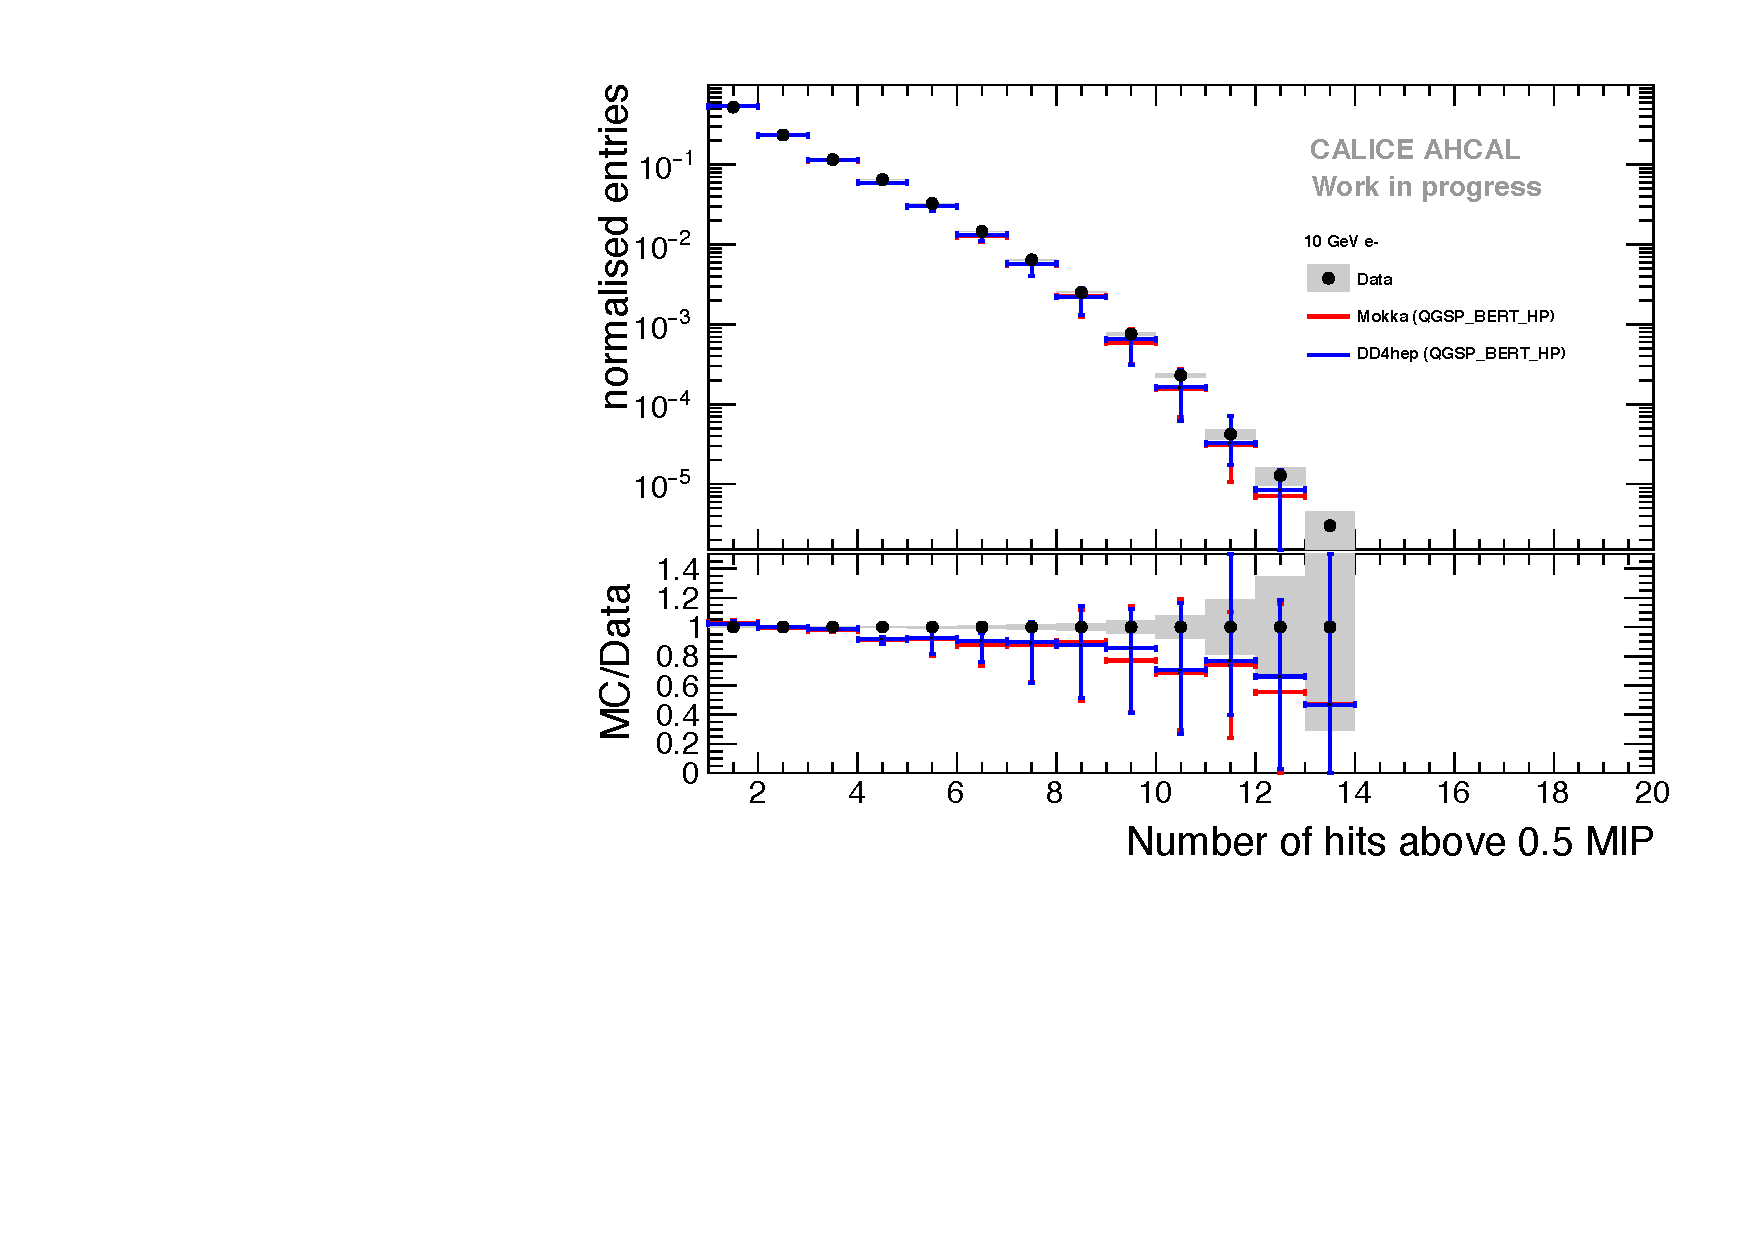
\includegraphics[width=0.5\textwidth]{fig/Electrons/Comparison_SimData_Electrons_nHits_10GeV.pdf}}\hfill
	\subfigure[15 GeV.\label{fig:elec_sim_data_nHits_15GeV}] {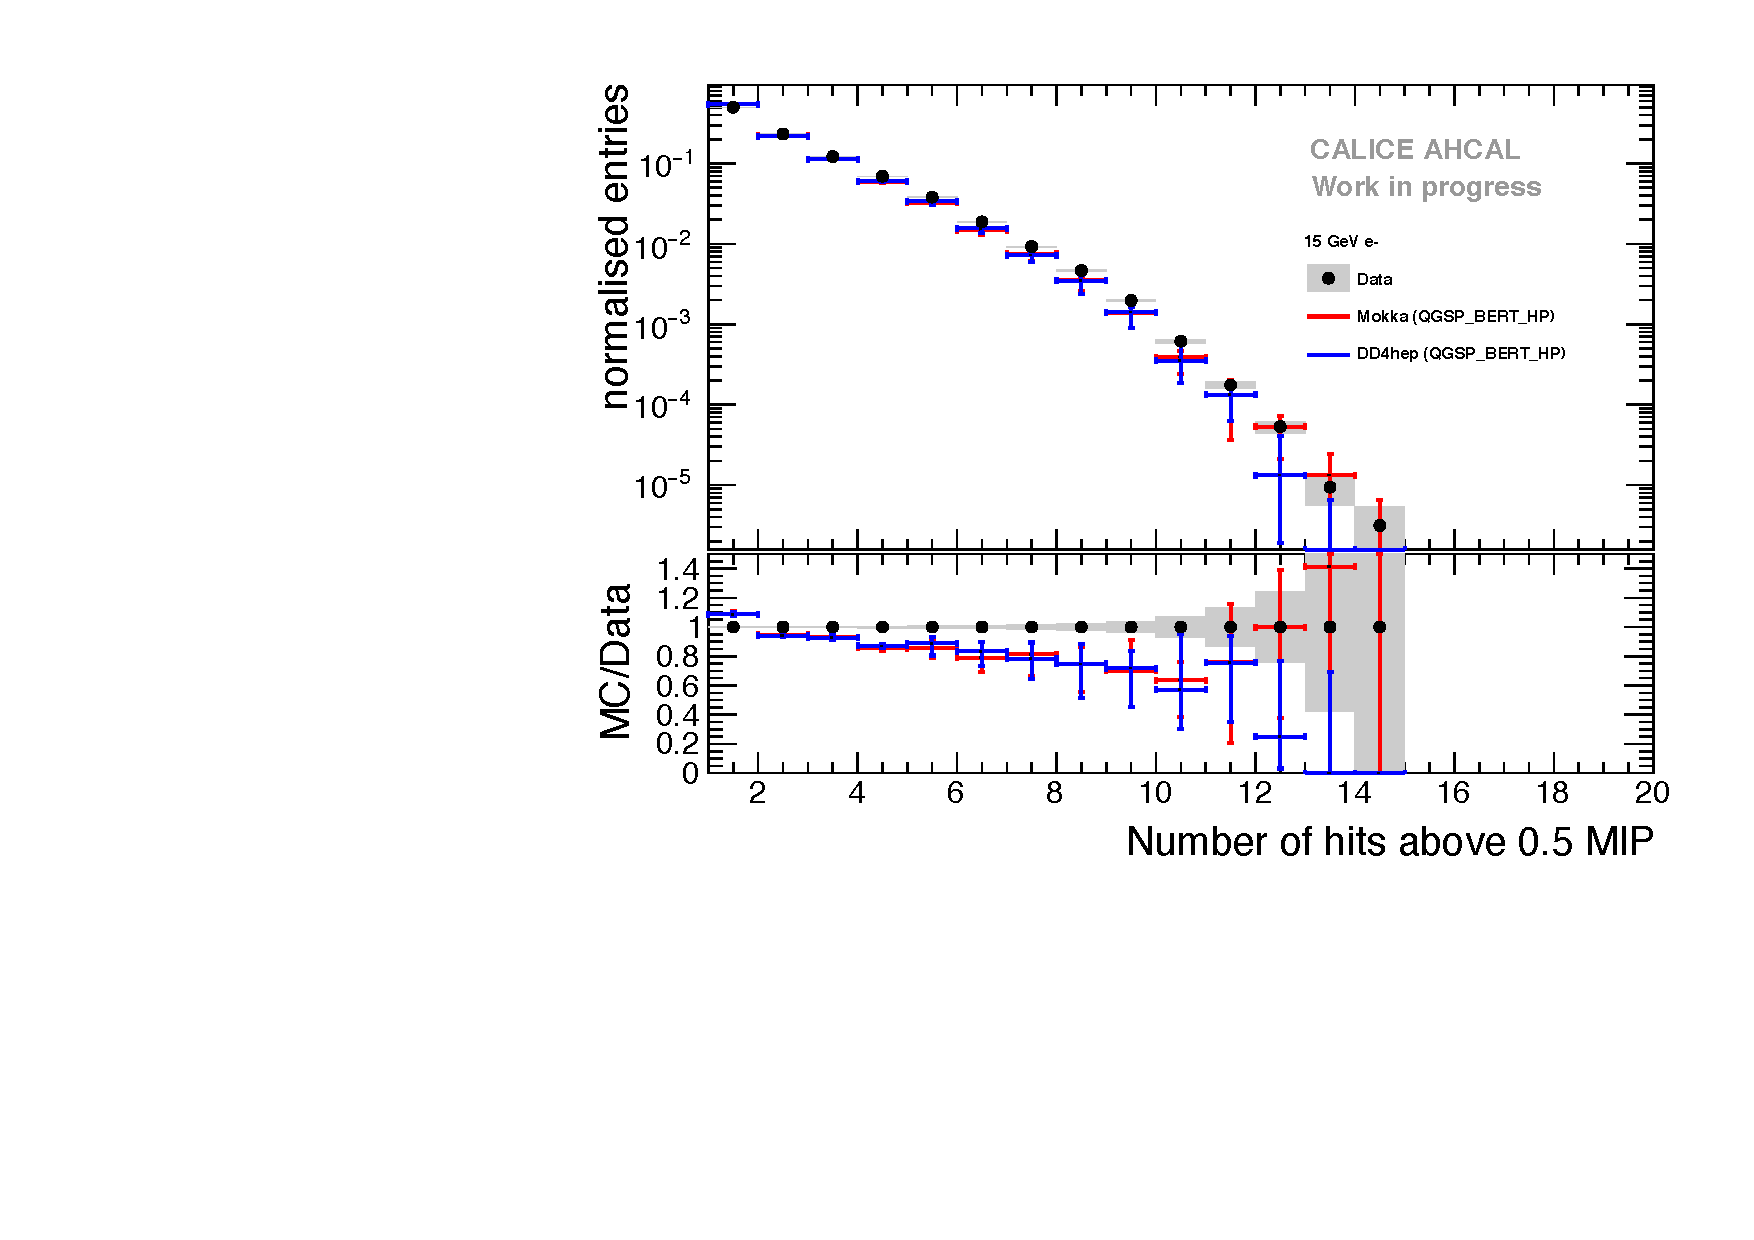
\includegraphics[width=0.5\textwidth]{fig/Electrons/Comparison_SimData_Electrons_nHits_15GeV.pdf}}\hfill
	\subfigure[20 GeV.\label{fig:elec_sim_data_nHits_20GeV}] {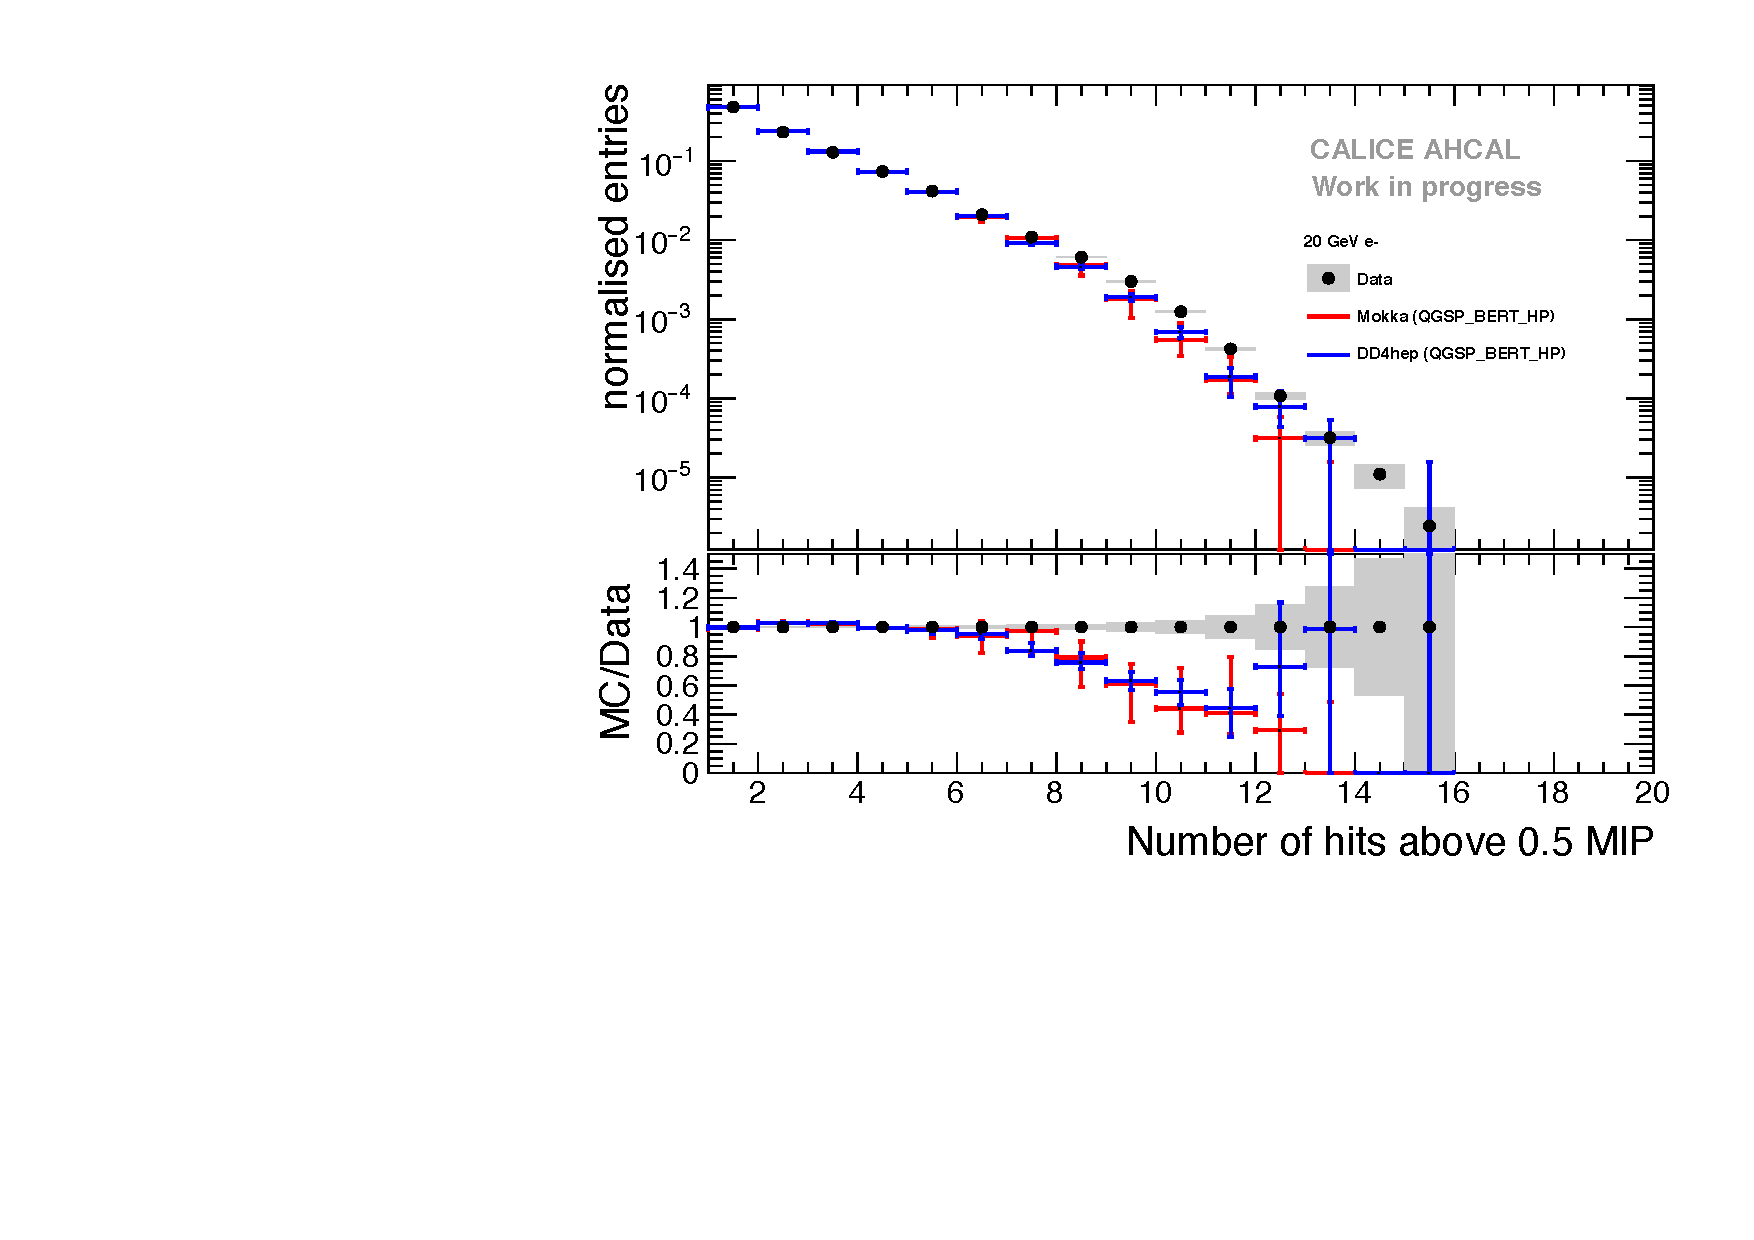
\includegraphics[width=0.5\textwidth]{fig/Electrons/Comparison_SimData_Electrons_nHits_20GeV.pdf}}\hfill
	\subfigure[30 GeV.\label{fig:elec_sim_data_nHits_30GeV}] {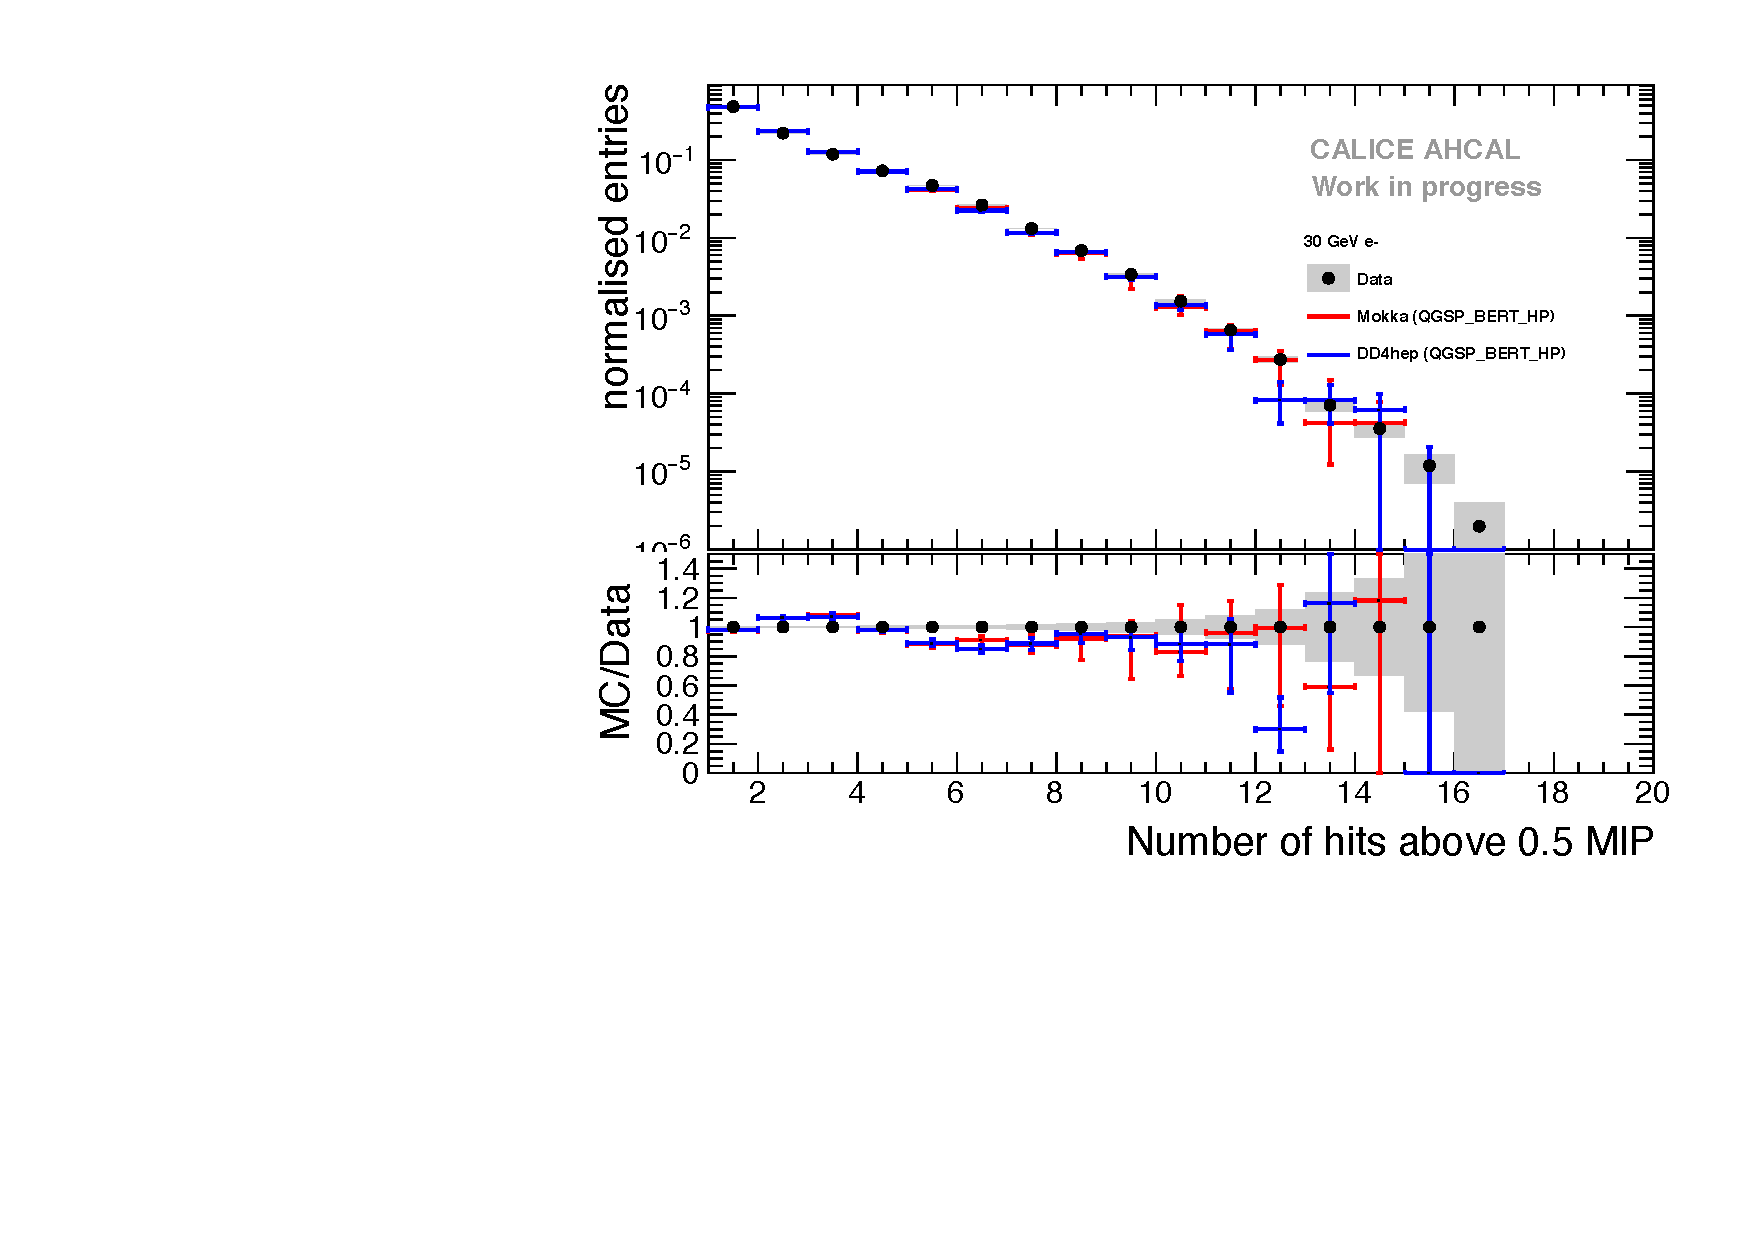
\includegraphics[width=0.5\textwidth]{fig/Electrons/Comparison_SimData_Electrons_nHits_30GeV.pdf}}\hfill
	\subfigure[40 GeV.\label{fig:elec_sim_data_nHits_40GeV}] {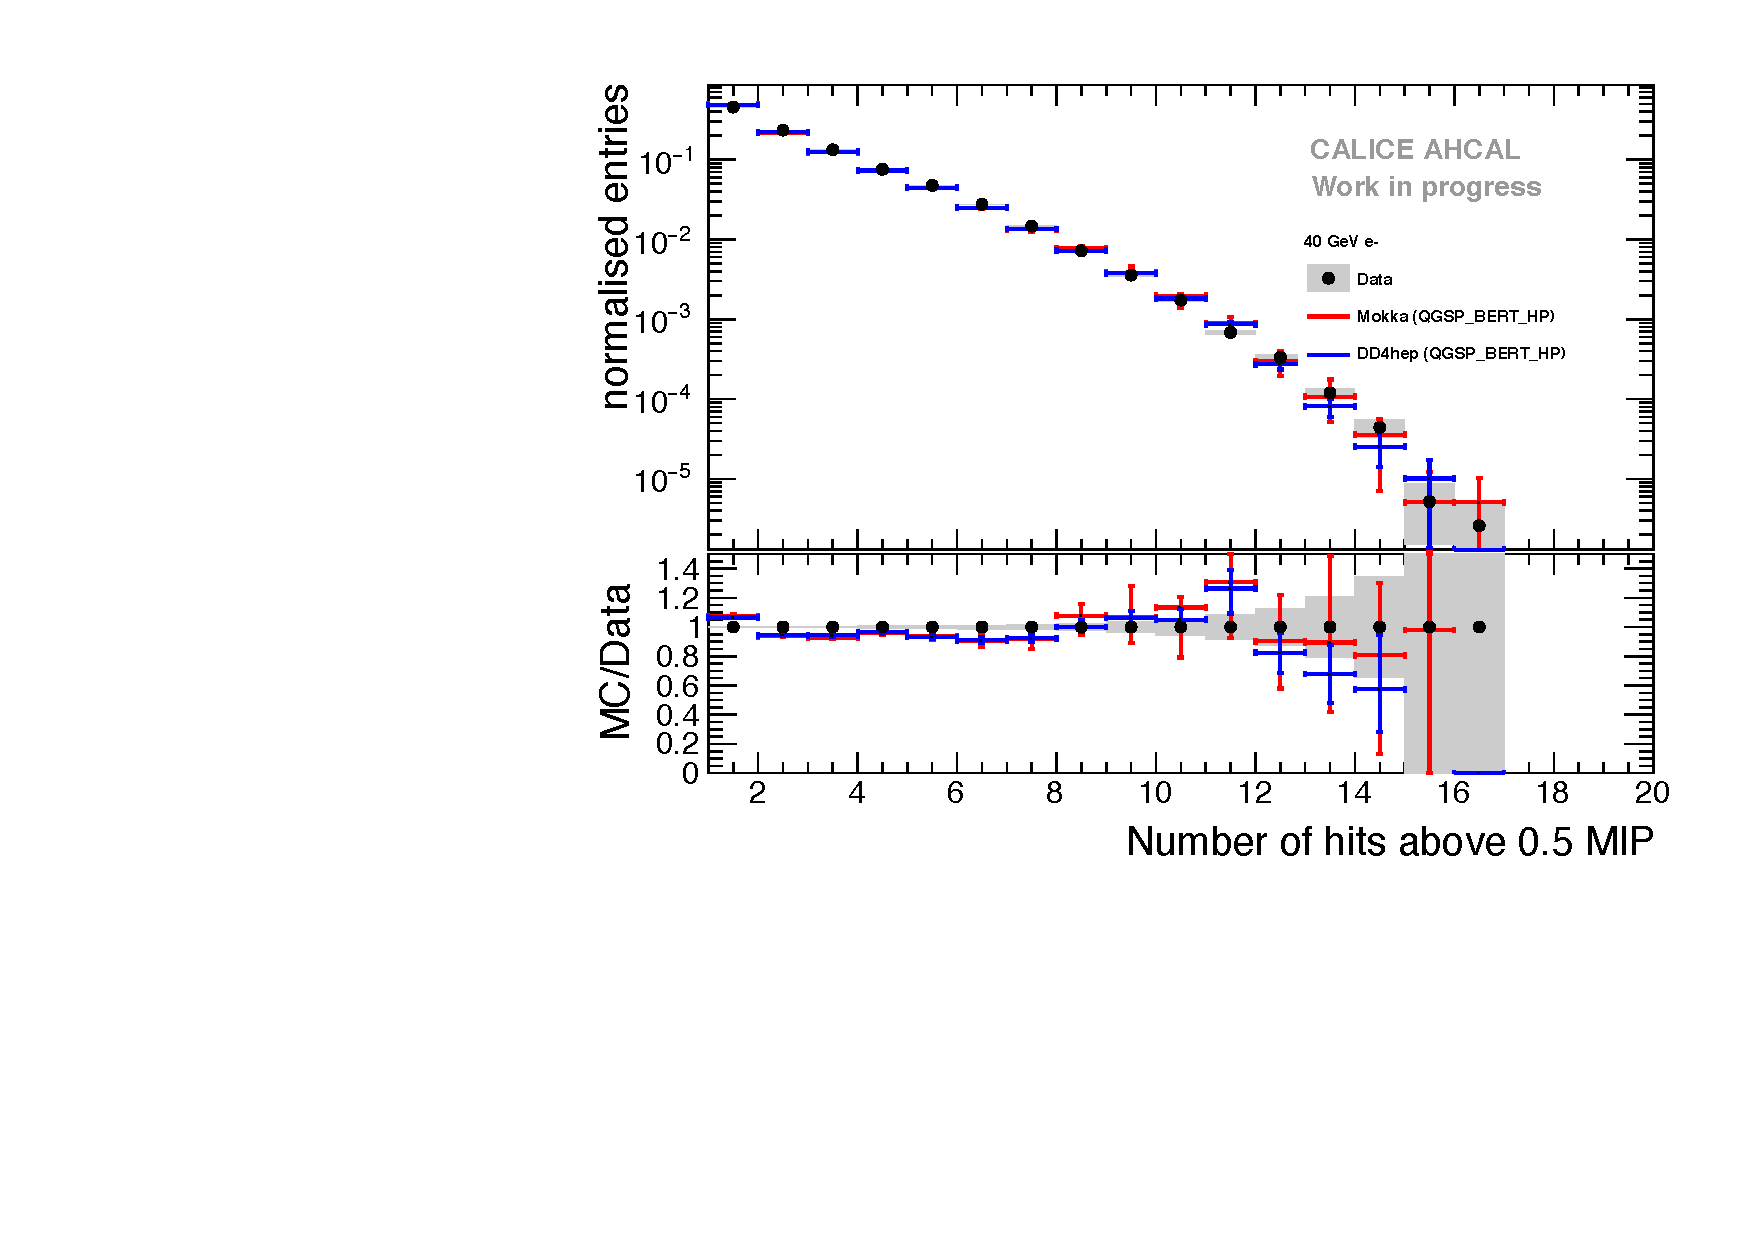
\includegraphics[width=0.5\textwidth]{fig/Electrons/Comparison_SimData_Electrons_nHits_40GeV.pdf}}\hfill
	\subfigure[50 GeV.\label{fig:elec_sim_data_nHits_50GeV}] {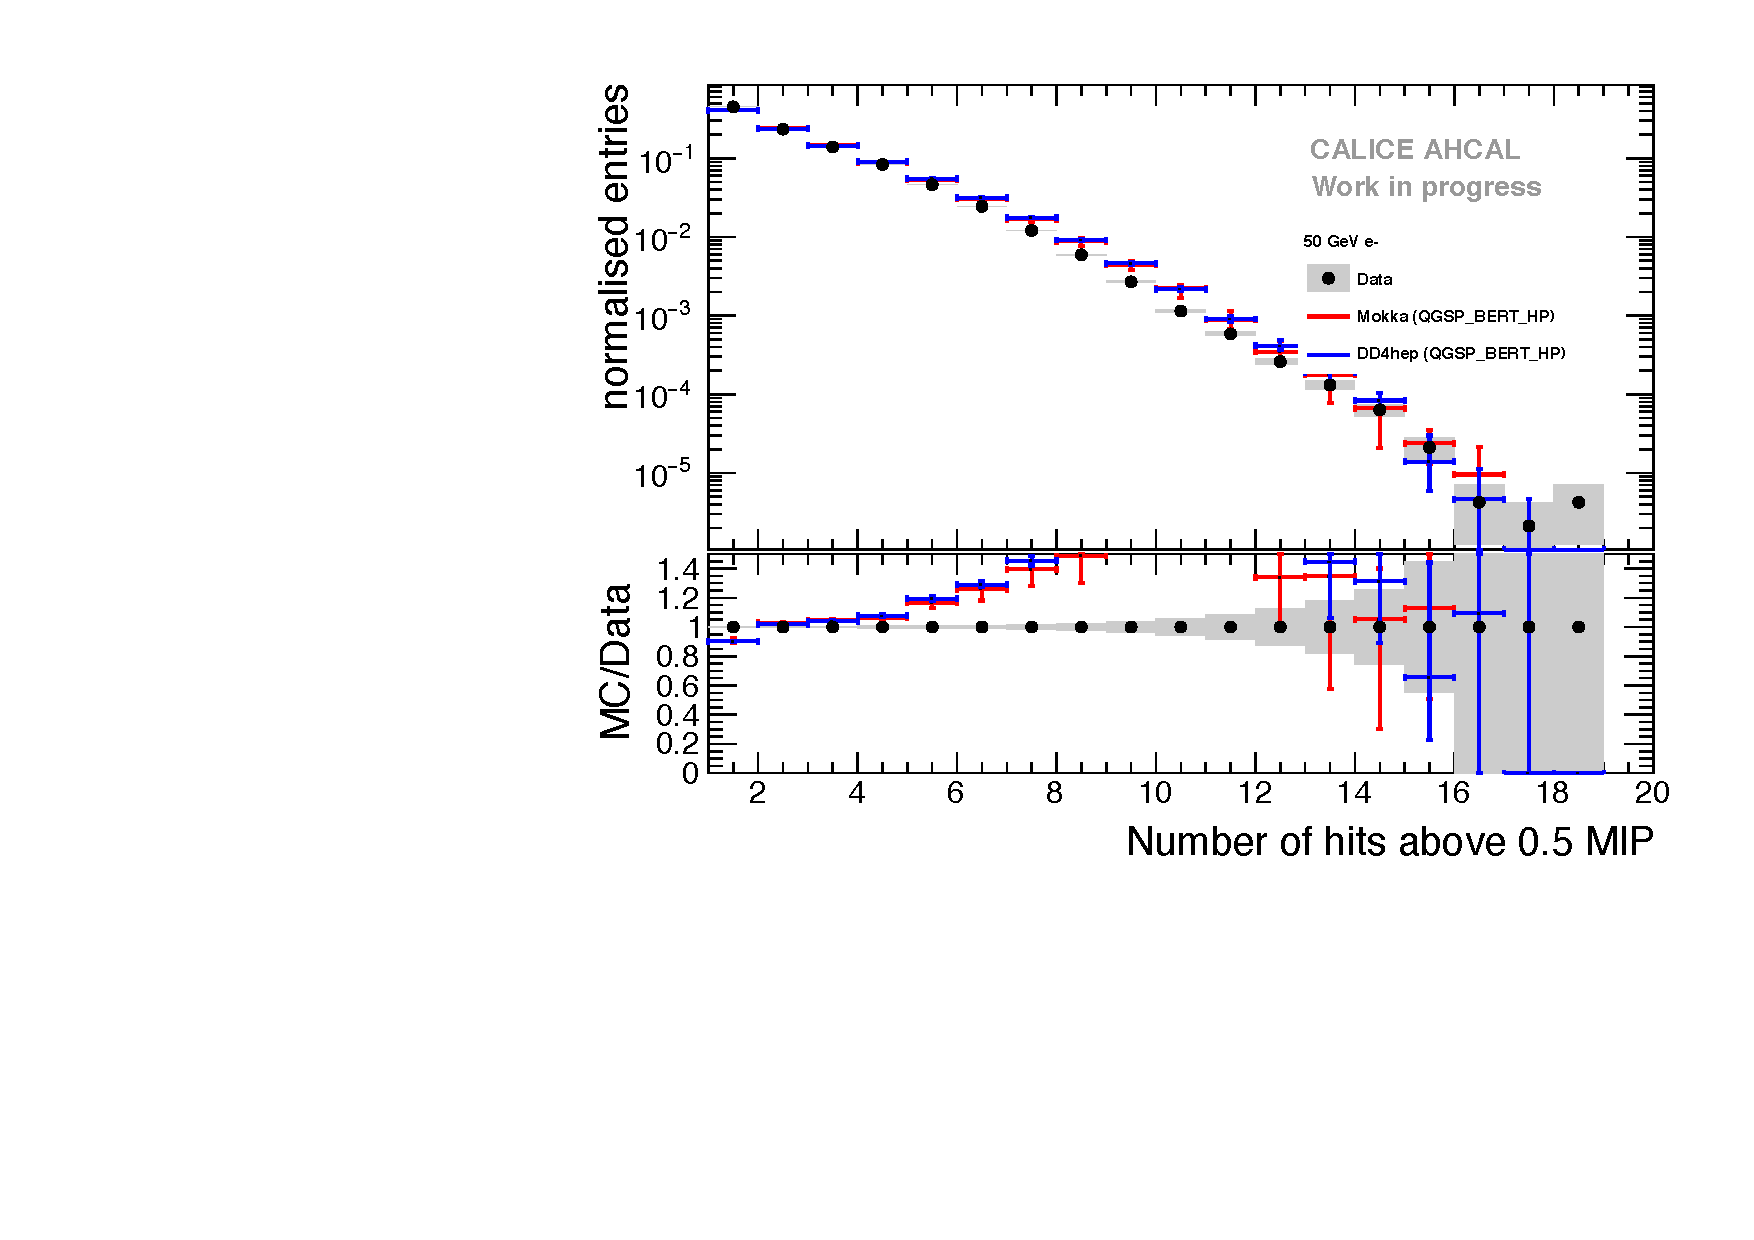
\includegraphics[width=0.5\textwidth]{fig/Electrons/Comparison_SimData_Electrons_nHits_50GeV.pdf}}\hfill
	\caption[]{Comparison between electron data and MC for all energies of the number of triggered channels per chip. The grey area represents the statistical error of the data. Error bars in simulation are obtained by varying the cross-talk parameter between 10\% and 18\%.}
	\label{fig:sim_data_elec_nHits}
\end{figure}
